%
%%%%%%%%%%%%%%%%%%%%%%%%%%%%%%%%%%%%%%%%%%%%%%%%%%%%%%%%%%%%%%%%%%%%%%%%%%%%%%%
% Kinematic differences between single and double $B$-hadron jetsDouble 
%%%%%%%%%%%%%%%%%%%%%%%%%%%%%%%%%%%%%%%%%%%%%%%%%%%%%%%%%%%%%%%%%%%%%%%%%%%%%%%
%
%\chapter{Kinematic differences between single and double $B$-hadron jets}
\chapter{Double $B$-hadron jet identification}\label{chap:kinematic}

%------------------------------------------------------------------------
%\section{Introduction}\label{sec:gbbintro}
%------------------------------------------------------------------------

%The purpose of this note is to describe the development of an algorithm to identify the $b$-jet flavor structure of single jets.  In particular, the proposed technique attempts to identify if the $b$-jet substructure is consistent with the decay of one or two $B$-hadrons within a single jet. There are two different strategies to approach this problem. One approach is to attempt to reconstruct multiple vertices originating from the decay of long-lived $B$-hadrons\cite{CDFAzimutalCorrelation}. % or use jet shape/substructure information. The former approach has low efficiency due to the double $b$-tag requirement that goes as the square of the $b$-tagging efficiency\cite{CDFAzimutalCorrelation}.

%In the present analysis we are exploring a different way to tag double $B$-hadron jets that does not rely on explicitly finding vertices but uses the jet shape/substructure information. Eventually, the goal should be to combine both approaches.

%------------------------------------------------------------------------
\section{Data and Monte Carlo samples}\label{sec:Simulation}
%------------------------------------------------------------------------


The tagging technique presented in this thesis relies on Monte Carlo predictions for the signal (single $b$) or background (merged $b$) hypotheses. The accuracy of the simulation is validated with data by comparing the distributions of the different variables explored.

Samples of jet events from proton-proton collision processes are simulated with {\sc Pythia8}~\cite{PYTHIA8} event generator using a $2\rightarrow 2$ matrix element at leading order in the strong coupling to model the hard subprocess, and $\pt$-ordered parton showers are utilized to model additional radiation in the leading-logarithmic approximation~\cite{Pythia_partonshowers}. Multiple parton interactions~\cite{Pythia_mpi}, as well as fragmentation and hadronisation based on the Lund string model~\cite{Lund_string_model} are also simulated.
%The proton parton distribution function (PDF) set used is the modified leading-order PDF set MRST LO*~\cite{}. 
The ATLAS MC11 tune of the soft model parameters was used~\cite{Pythia_MC11tune}.
In order to have sufficient statistics over the entire $\pt$ spectrum, eight samples were generated with different thresholds of the hard-scattering partonic transverse momentum $\hat{p}_T$. Events from different samples were mixed taking into account their respective production cross sections.

%After the event generation, the events are passed through a full {\sc Geant4}~\cite{GEANT4} detector simulation with a detailed description of the geometry and the material of the ATLAS experiment, and %QGSP$\_$BERT~\cite{QGSP, BERT} asthe set of processes describing the hadronic interactions.
%using Bertini Cascades~\cite{QGSP, BERT} for the modeling of interactions of high energy hadrons. 
The {\sc Geant4}~\cite{GEANT4} software toolkit within the ATLAS simulation framework~\cite{ATLASSimulation} propagates the generated particles through the ATLAS detector and simulates their interactions with the detector material. The energy deposited by particles in the active detector material is converted into detector signals in the same format as the detector read-out. Finally the Monte Carlo generated events are processed through the trigger simulation package of the experiment, and are reconstructed and analyzed with the same software as for the real data.
The simulated data sample used for the analysis %(MC11b)
gives an accurate description of the pile-up content and detector conditions for the full 2011 data-taking period. 

The data samples employed correspond to proton-proton collisions at $\sqrt{s}=7$ TeV delivered by the LHC and recorded by ATLAS between May and November 2011, with the LHC running with 50~ns bunch spacing, and bunches organized in bunch trains. Only data collected during stable beam periods in which all sub-detectors were fully operational are used.  After the application of the data quality selection, % the total integrated luminosity is about  4.7 fb$^{-1}$.  
the surviving data corresponds to an integrated luminosity of 4.7~fb$^{-1}$. The LHC performance steadily improved during 2011. In particular  the average number of minimum-bias pile-up events, originating from collisions of additional protons in the same bunch as the signal collision, grew from from 3 to 20. This fact will be of importance when discussing the selection of discriminating variables.  
%the average number of interactions per bunch crossing throughout the data-taking period considered was approximately $3 \leq  \mu \leq 8$ until summer 2011, with a global average for this period of $\mu \approx 6$. Starting in August 2011 and lasting through the end of the proton run, $\mu$ ranged from approximately 5 to 17, with an average of about 12. 

For the study of systematic effects and for result comparison, other Monte Carlo samples were utilised. Results were produced with the {\sc herwig}++  generator~\cite{Herwig} and with {\sc Pythia8} using the Perugia tune~\cite{Perugia}. The former is based on the event generator {\sc herwig}, but redesigned in the $C$++ programming language. The generator contains a few modlleing improvements. It also uses angular-ordered parton showers, but with an updated evolution variable and a better phase space treatment. Hadronisation is perfromed using the cluster model. The underlying event and soft inclusive interactions are described using a hard and soft multiple partonic interactions model~\cite{Bahr:2008dy}. The Perugia tune is an independent tune of {\sc pythia} with increased final state radiation to better reproduce the jet shapes and hadronic event shapes using LEP and {\sc tevatron} data. In addition, paramteres sensitive to the production of particles with strangeness and related to jet fragmentation have been adjusted.


%en realidad voy a referir al capitulo donde describo los distintos MC generators y voy a decir
%The Monte Carlo event generators discussed in Section... are used here. 
%Pythia, pythia with the Perugia tune and herwig++ where these are used both for the simulation of the hard 2-2 process as well as for the parton shower, underlying event, and hadrnisation models.


%------------------------------------------------------------------------
\section{Event and object selection}\label{sec:EventSelection}
%------------------------------------------------------------------------

%In this section we examine the procedure for event selection and the conditions that the calorimeter jets must satisfy in order to be considered.

%%% The following was taken from this BTagging note, https://cdsweb.cern.ch/record/1435194
%%% from 2012! 
The event sample for this analysis was collected  using a logical OR of single jet triggers which select events with at least one jet with transverse energy above a given threshold at the highest trigger level. The ATLAS Trigger system uses three consecutive trigger levels. At the hardware Level 1 and local software Level 2, cluster-based jet triggers are used to select events. The Level 3, the so-called Event Filter, runs  the offline anti-$k_t$ jet finding algorithm with $R = 0.4$ on topological clusters over the complete calorimeter.  At this stage, the transverse energy thresholds, expressed in GeV, are: 20, 30, 40, 55, 75, 100, 135, 180. These triggers reach an efficiency of 99\% for events having the leading jet with an offline energy higher than the corresponding trigger thresholds by a factor ranging between 1.5 and 2. The triggers with the lowest $\pt$ thresholds were prescaled by up to five orders of magnitude, and typically the same jet trigger is prescaled ten times more in the later data taking periods compared to the early ones. %The offline event selection consists of requiring at least one primary vertex candidate to have 5 or more tracks. 

%Only events with exactly two B hadrons were considered.

%Monte Carlo jets belong to the QCD simulation described in section~\ref{sec:Simulation}.

The offline event selection requires at least one primary vertex candidate with 5 or more tracks. All jets, with transverse momentum between 40 and 480~GeV,  %, reconstructed with the anti-$k_t$ $R=0.4$ algorithm built from topological clusters, 
were required to be in a region with full tracking coverage, $|\eta_{jet}|<2.1$, and they were classified in eight $\pt$ bins chosen such as to match the jet trigger 99\% efficiency thresholds (in GeV): 40, 60, 80, 110, 150, 200, 270, 360.  %The trigger strategy is detailed in Table~\ref{tab:trigger}. 
 Only jets tagged as $b$-jets using the MV1 $b$-tagging algorithm at the 60\% efficiency working point were considered. $b$-tagged jets with close-by jets ($\Delta R < 0.8$) with $\pt$ higher than 7~GeV at electromagnetic scale were not included in the analysis. Unless otherwise indicated, performance plots are shown for one medium  $\pt$ bin (80 to 110~GeV) and one high $\pt$ bin (200 to 270~GeV).


In the case of MC the reconstructed $b$-tagged jets were further classified into single and merged $b$-jets based on truth Monte Carlo information. A $B$-hadron is considered to be associated to a jet if the $\Delta R$ distance in $\eta-\phi$ space between the direction of the hadron and the jet axis is smaller than 0.4. Jets were labeled as merged (single) $b$-jets if they contain two (only one) $B$-hadron.%\footnote[2]{Another approach is to match particles using the 'active area' of the jet, defined with the concept of ghost-particles but utilizing true particles as ghost constituents\cite{CatchmentArea}. This procedure will be implemented in a future version of this analysis.}.

 


%\begin{table}
%\renewcommand{\arraystretch}{1.3}
%\centering
%{\small
%\begin{tabular}{|   c   |   c   |   c   |}
%\hline $\pt$ (GeV) & Run 177531 - 187109 & Run $>$ 187109 \\  \hline
%%(30,40)     & EF\_j15\_a4\_EFFS  OR  EF\_j10\_a4\_EFFS  & EF\_j15\_a4tc\_EFFS OR  EF\_j10\_a4tc\_EFFS   \\ \hline \hline
%(40,60)     & EF\_j20\_a4\_EFFS  OR  EF\_j15\_a4\_EFFS  & EF\_j20\_a4tc\_EFFS OR  EF\_j15\_a4tc\_EFFS   \\ 
%(60,80)     & EF\_j30\_a4\_EFFS  OR  EF\_j20\_a4\_EFFS  & EF\_j30\_a4tc\_EFFS OR  EF\_j20\_a4tc\_EFFS   \\ 
%(80,110)    & EF\_j40\_a4\_EFFS  OR  EF\_j30\_a4\_EFFS  & EF\_j40\_a4tc\_EFFS OR  EF\_j30\_a4tc\_EFFS   \\ 
%(110,150)   & EF\_j55\_a4\_EFFS  OR  EF\_j40\_a4\_EFFS  & EF\_j55\_a4tc\_EFFS OR  EF\_j40\_a4tc\_EFFS   \\ 
%(150,200)   & EF\_j75\_a4\_EFFS  OR  EF\_j55\_a4\_EFFS  & EF\_j75\_a4tc\_EFFS OR  EF\_j55\_a4tc\_EFFS   \\ 
%(200,270)   & EF\_j100\_a4\_EFFS OR  EF\_j75\_a4\_EFFS  & EF\_j100\_a4tc\_EFFS OR  EF\_j75\_a4tc\_EFFS  \\ 
%(270,360)   & EF\_j135\_a4\_EFFS OR  EF\_j100\_a4\_EFFS & EF\_j135\_a4tc\_EFFS OR  EF\_j100\_a4tc\_EFFS \\ 
%(360,480)   & EF\_j180\_a4\_EFFS OR  EF\_j135\_a4\_EFFS & EF\_j180\_a4tc\_EFFS OR  EF\_j135\_a4tc\_EFFS \\ %\hline \hline
%$>$480     & EF\_j240\_a4\_EFFS OR  EF\_j180\_a4\_EFFS & EF\_j240\_a4tc\_EFFS OR  EF\_j180\_a4tc\_EFFS \\
%\hline
%\end{tabular}
%}
%\caption{The \pt\ bins used in the present analysis and the respective triggers the must satisfy.}
%\label{tab:trigger}
%\end{table}



%------------------------------------------------------------------------
%\section{Track selection }\label{sec:TrackSelection}
%------------------------------------------------------------------------

It is important to select genuine tracks belonging to jets. Only tracks located  within a cone of radius $\Delta R(jet^{\rm reco},\rm track) \leq 0.4$ around the jet axis were considered. %\footnote[2]{In a future version of the study the concept of ghost-particles\cite{CatchmentArea} can be applied in the track-to-jet assignment using tracks as ghost constituents.}.
  Cuts on $p_{\rm{T}}^{\rm{trk}}>1.0$~GeV and the $\chi^2$ of the track fit, $\chi^2/{\it ndf}<3$, are applied. % as a minimum starting point. 
 In addition, tracks are required to have a total of at least seven precision hits (pixel or micro-strip) in order to guarantee at least 3 $z$-measurements. Tracks are also required to fulfill cuts on the transverse and longitudinal impact parameters at the perigee to ensure that they arise from  the primary vertex. As cutting on impact parameter (IP) significance might be detrimental for $b$-jets, where large IP values are expected, the relaxed cuts were used, $|IP_{xy}|<2$~mm, and $|IP_{z}\sin\theta|<2$~mm, with $\theta$ being the polar angle measured with respect to the beam axis. %This, however, might still be too tight for $b$-jets.



%------------------------------------------------------------------------
%\section{Kinematid differences between single $b$- and merged $b\bar{b}$-jets}\label{sec:gbbKine}
\section{Preliminary studies in standalone {\sc pythia} generator}\label{sec:gbbKine}
%------------------------------------------------------------------------ 


A small set of dijet events was generated using {sc pythia}. With the help of fastjet~\cite{fastjet}, anti-$k_t$ jets with distance parameters $R$ of 0.4 and 0.6 were built using as inputs:

\begin{itemize}\addtolength{\itemsep}{-0.4\baselineskip}
\item
all stable particles
\item
charged stable particles
\item 
0.1 $k_t$ jets, using all particles 
\item 
0.1 $k_t$ jets, using charged particles 
\end{itemize}

The labeling was done in the same procedure as in the Full ATLAS Monte Carlo analysis.

Figures~\ref{fig:pythiaTrkWidthAnkt4and6} to~\ref{fig:CorrTau1Tau2DRkt} show the distributions and correlations of some of the tracking variables, for single and merged $b$-jets, in bins of the jet $\pt$.


\begin{figure}[tp]
\centering
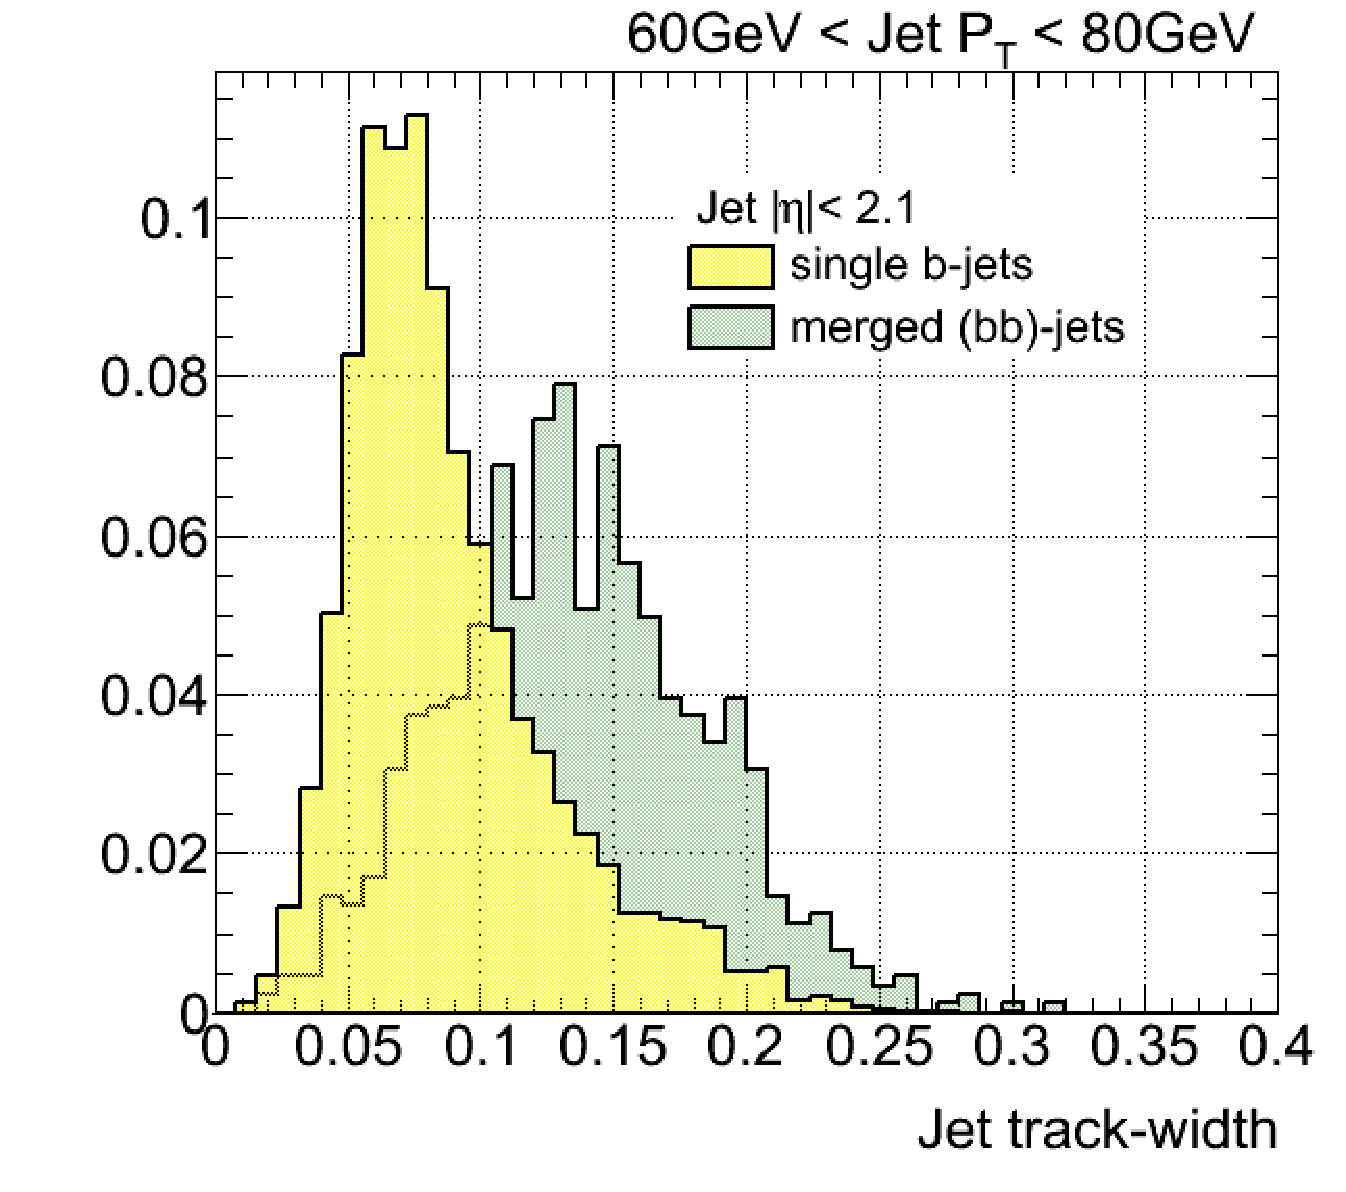
\includegraphics[width=0.49\textwidth]{FIGS/TEMPFigs/PythisStandalone/Antikt4/allparticles/trkWidth060.pdf}
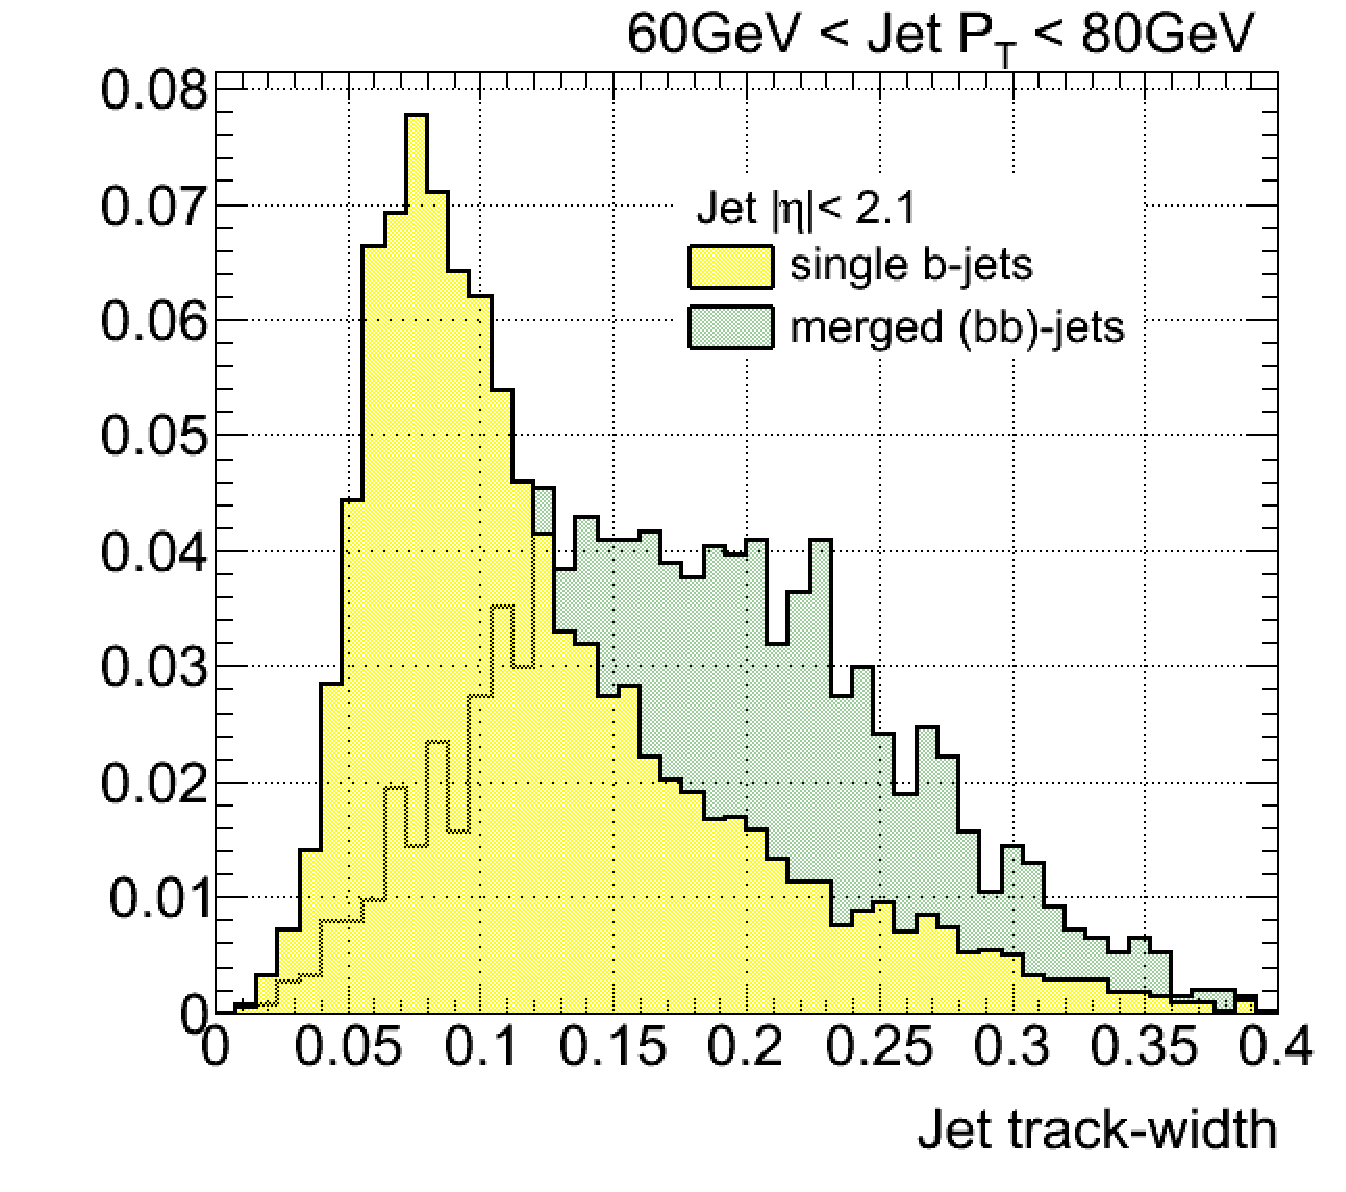
\includegraphics[width=0.49\textwidth]{FIGS/TEMPFigs/PythisStandalone/Antikt6/allparticles/trkWidth060.pdf}
\caption{Distribution of track-jet width in anti-$k_T$ 0.4 (left) and 0.6 (right) jets, for single and merged $b$-jets between 60~GeV to 80~GeV. Jets were built using all stable particles in the simulation.}
\label{fig:pythiaTrkWidthAnkt4and6}
\end{figure}

\begin{figure}[tp]
\centering
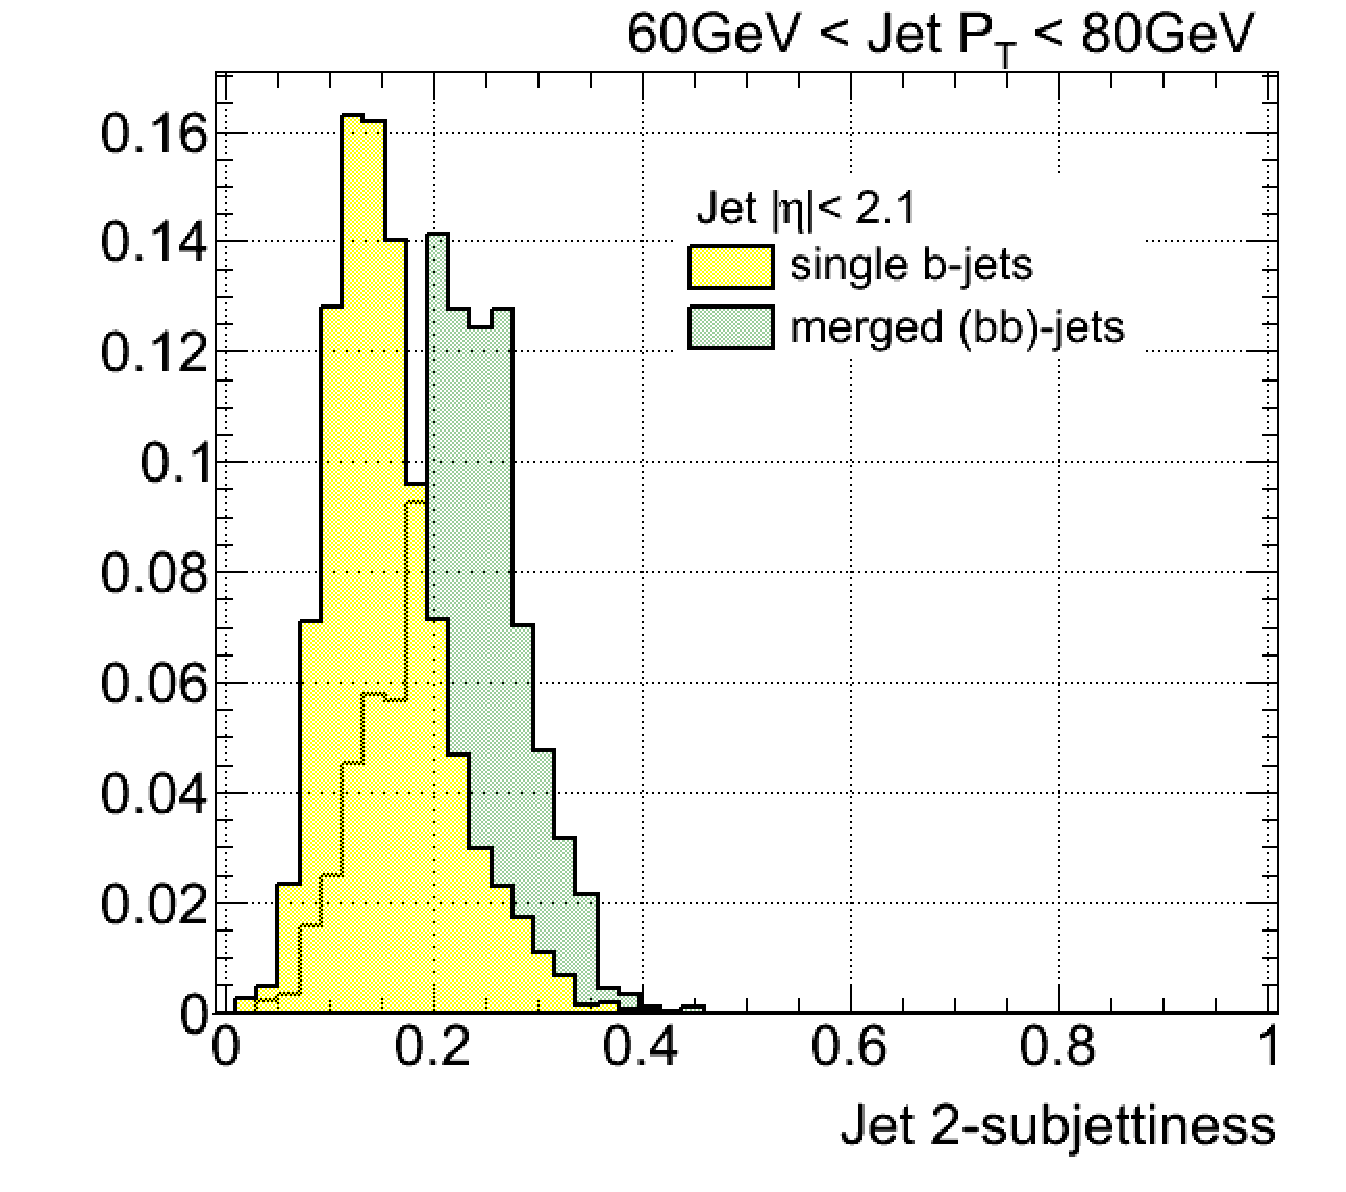
\includegraphics[width=0.49\textwidth]{FIGS/TEMPFigs/PythisStandalone/Antikt4/allparticles/Tau2060.pdf}
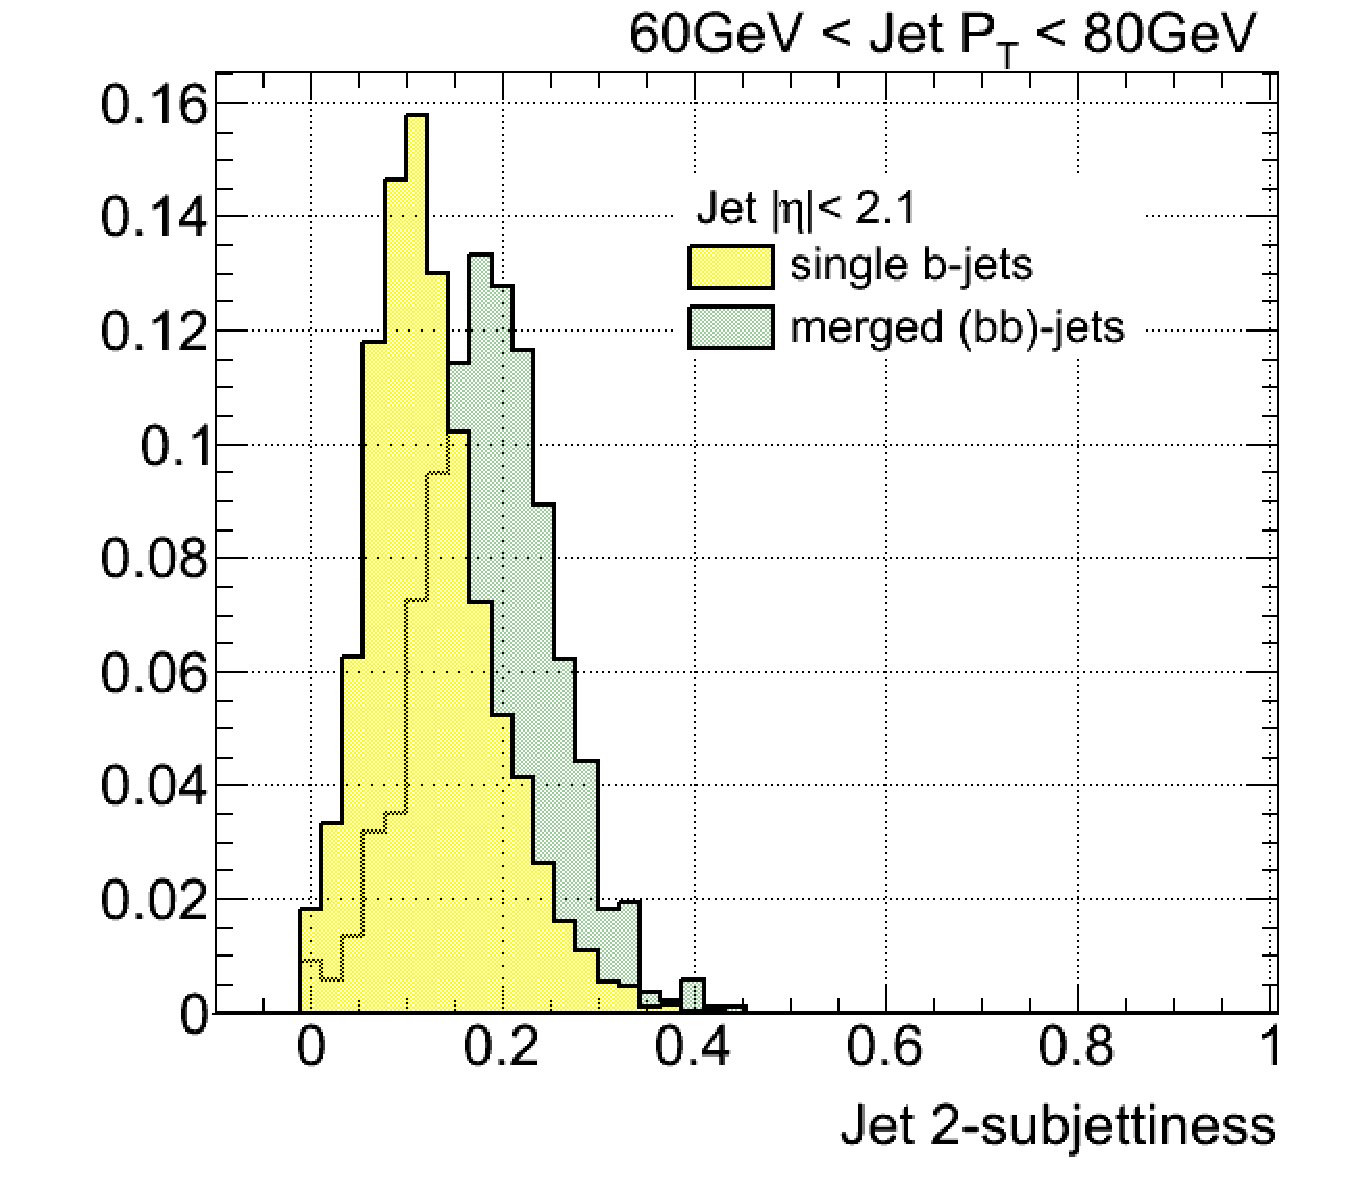
\includegraphics[width=0.49\textwidth]{FIGS/TEMPFigs/PythisStandalone/Antikt4/chargedparticles/Tau2060.pdf}
\caption{Distribution of $\tau_2$ in anti-$k_T$ 0.4 jets, for single and merged $b$-jets between 60~GeV to 80~GeV. Jets were built using all stable particles (left) and charged particles only (right).}
\label{fig:pythiaTau2AllandCharged}
\end{figure}

\begin{figure}[tp]
\centering
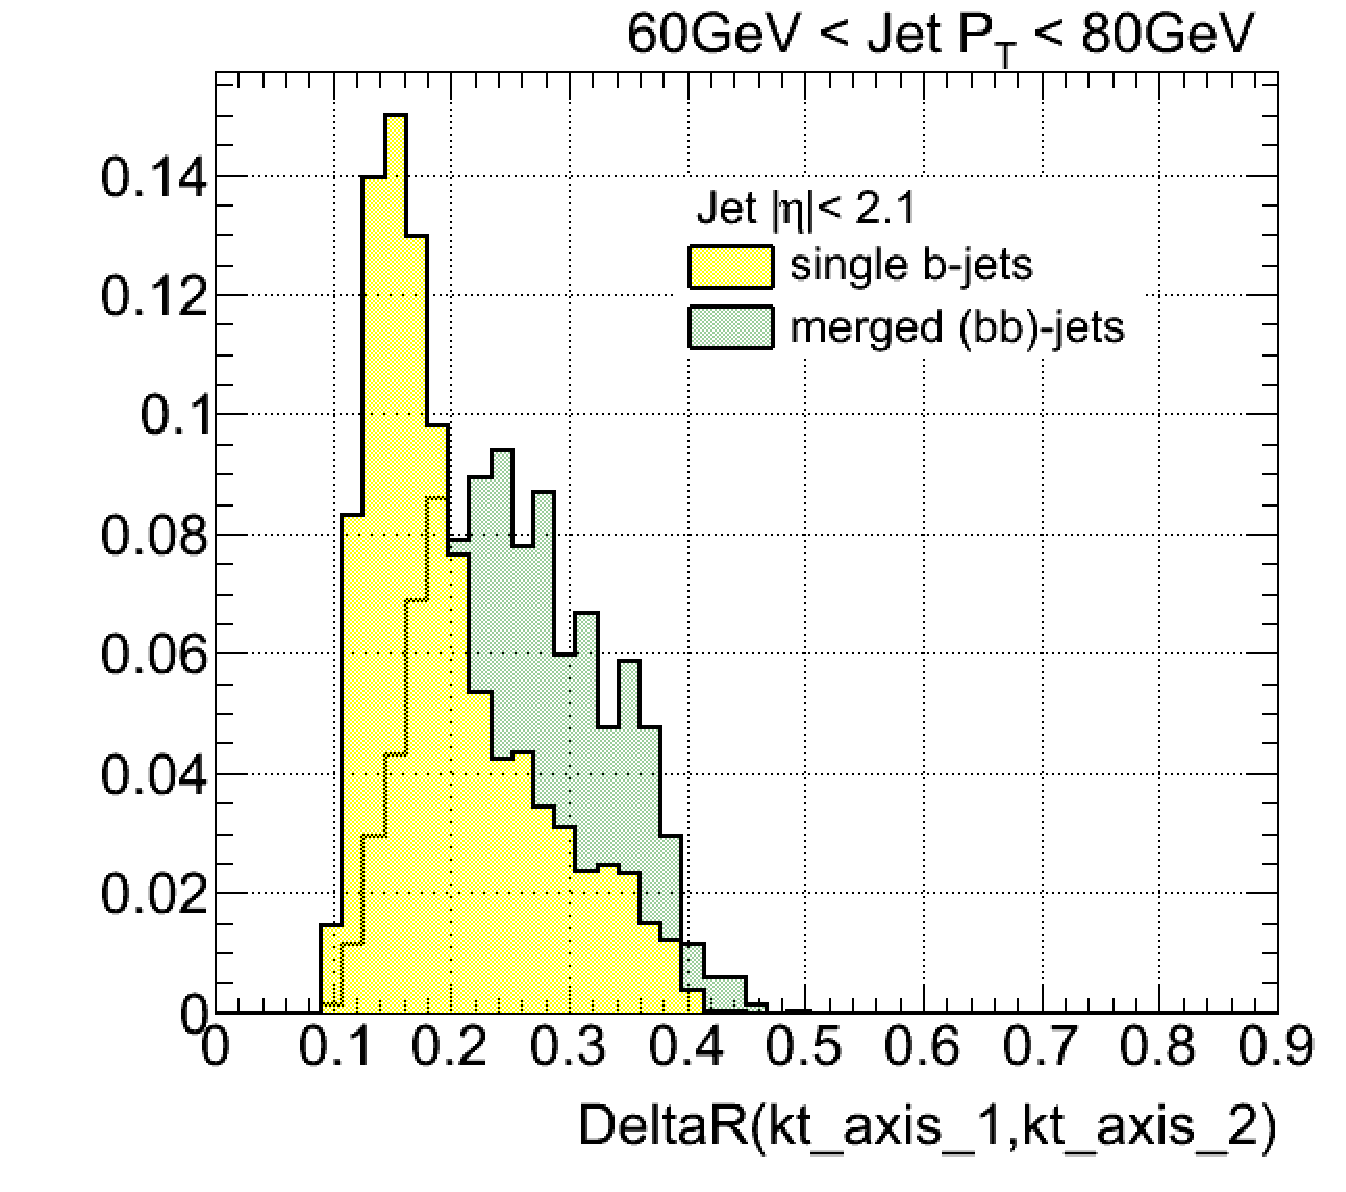
\includegraphics[width=0.49\textwidth]{FIGS/TEMPFigs/PythisStandalone/Antikt4/minijets/DRkt2axes060.pdf}
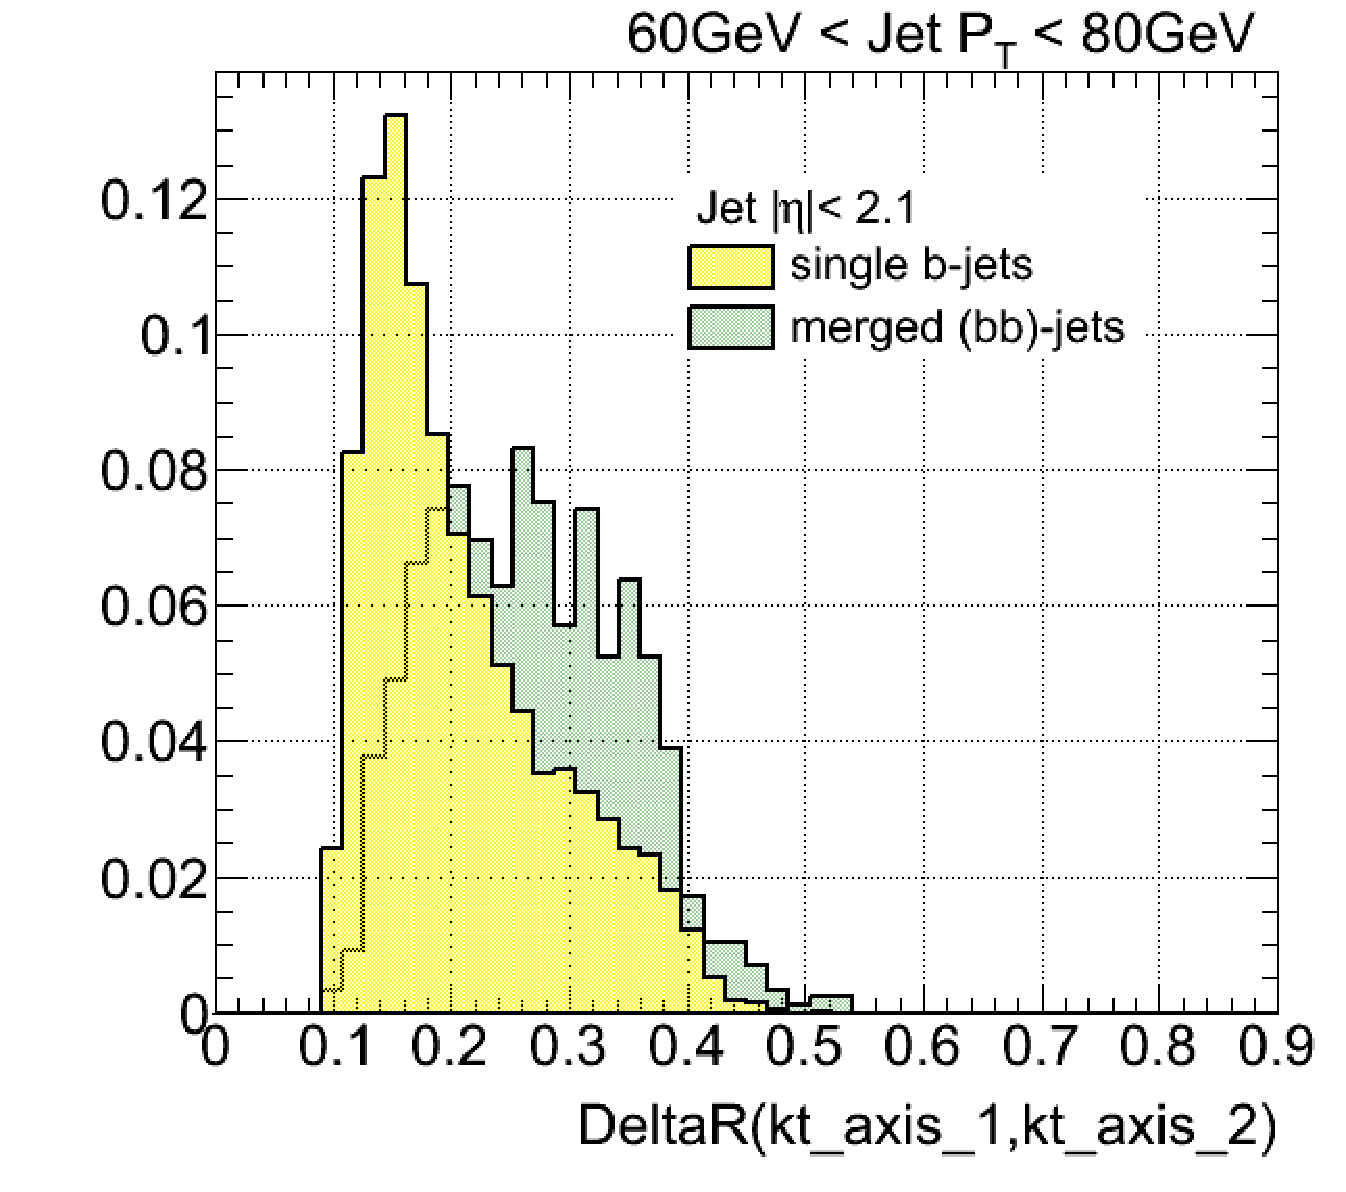
\includegraphics[width=0.49\textwidth]{FIGS/TEMPFigs/PythisStandalone/Antikt4/chargedminijets/DRkt2axes060.pdf}
\caption{Distribution of $\Delta R$ between the axes of two $k_T$ subjets in anti-$k_T$ 0.4 jets, for single and merged $b$-jets between 60~GeV to 80~GeV. Jets were built using 0.1 $k_t$ jets from all stable particles (left) and charged particles only (right).}
\label{fig:pythiaDRktAllJetandChargedJet}
\end{figure}

\begin{figure}[tp]
\centering
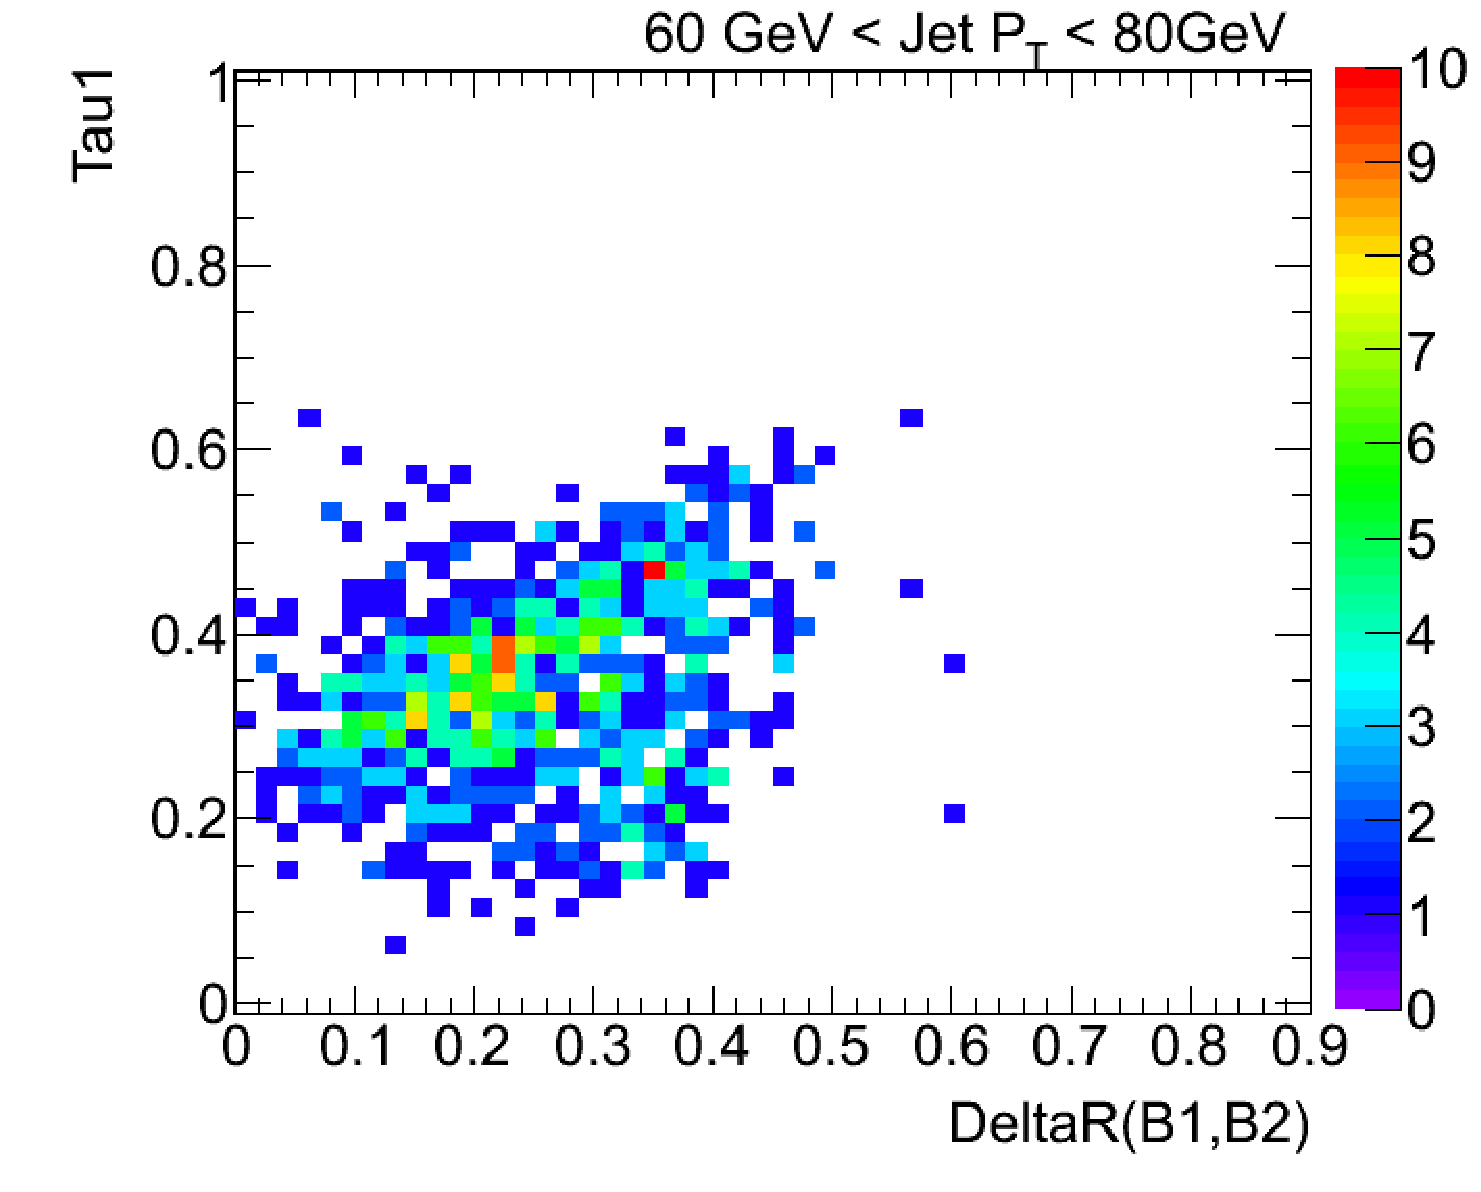
\includegraphics[width=0.49\textwidth]{FIGS/TEMPFigs/PythisStandalone/Antikt4/allparticles/Tau1DeltaRCorr_PT60.pdf}
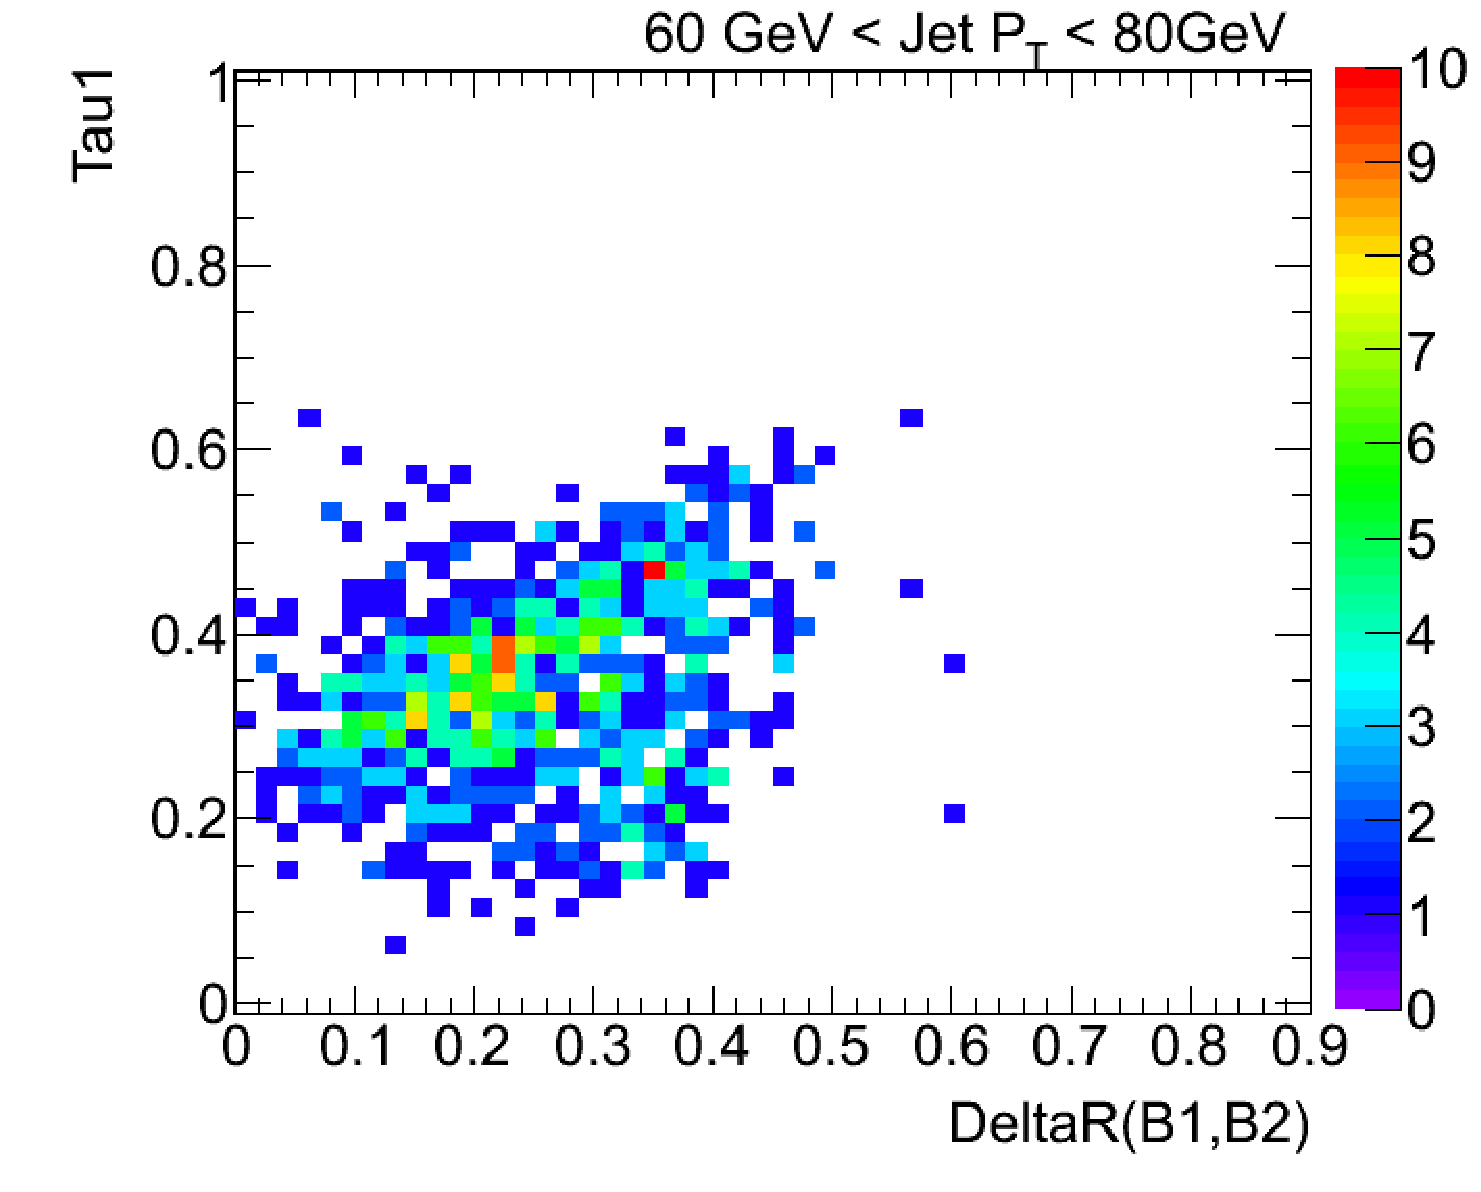
\includegraphics[width=0.49\textwidth]{FIGS/TEMPFigs/PythisStandalone/Antikt4/allparticles/Tau1DeltaRCorr_PT60.pdf}
\caption{Correlation between $\tau_1$ (left) and $\tau_2$ (right) and the $\Delta R$ between the $B$-hadrons in merged anti-$k_T$ 0.4 jets  between 60~GeV to 80~GeV. Jets were built using all stable particles.}
\label{fig:CorrTau1Tau2DRBB}
\end{figure}

\begin{figure}[tp]
\centering
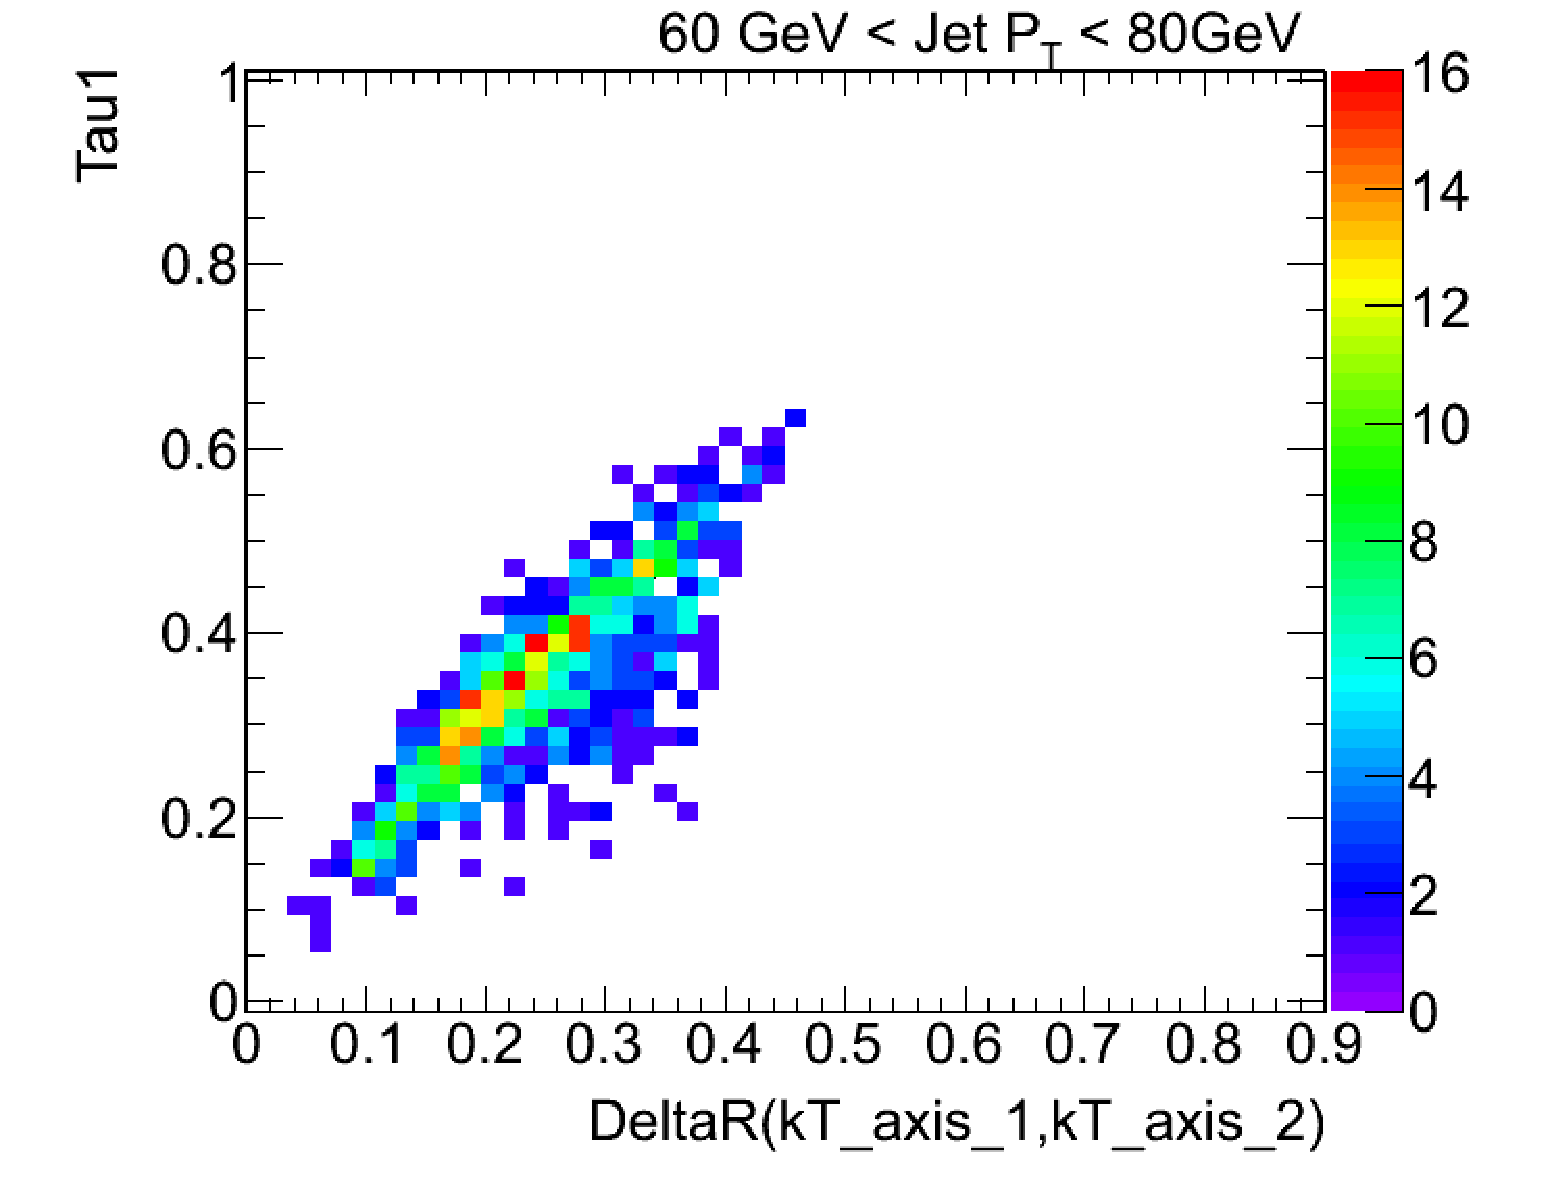
\includegraphics[width=0.49\textwidth]{FIGS/TEMPFigs/PythisStandalone/Antikt4/allparticles/Tau1DRkT2axesCorr_PT60_merged.pdf}
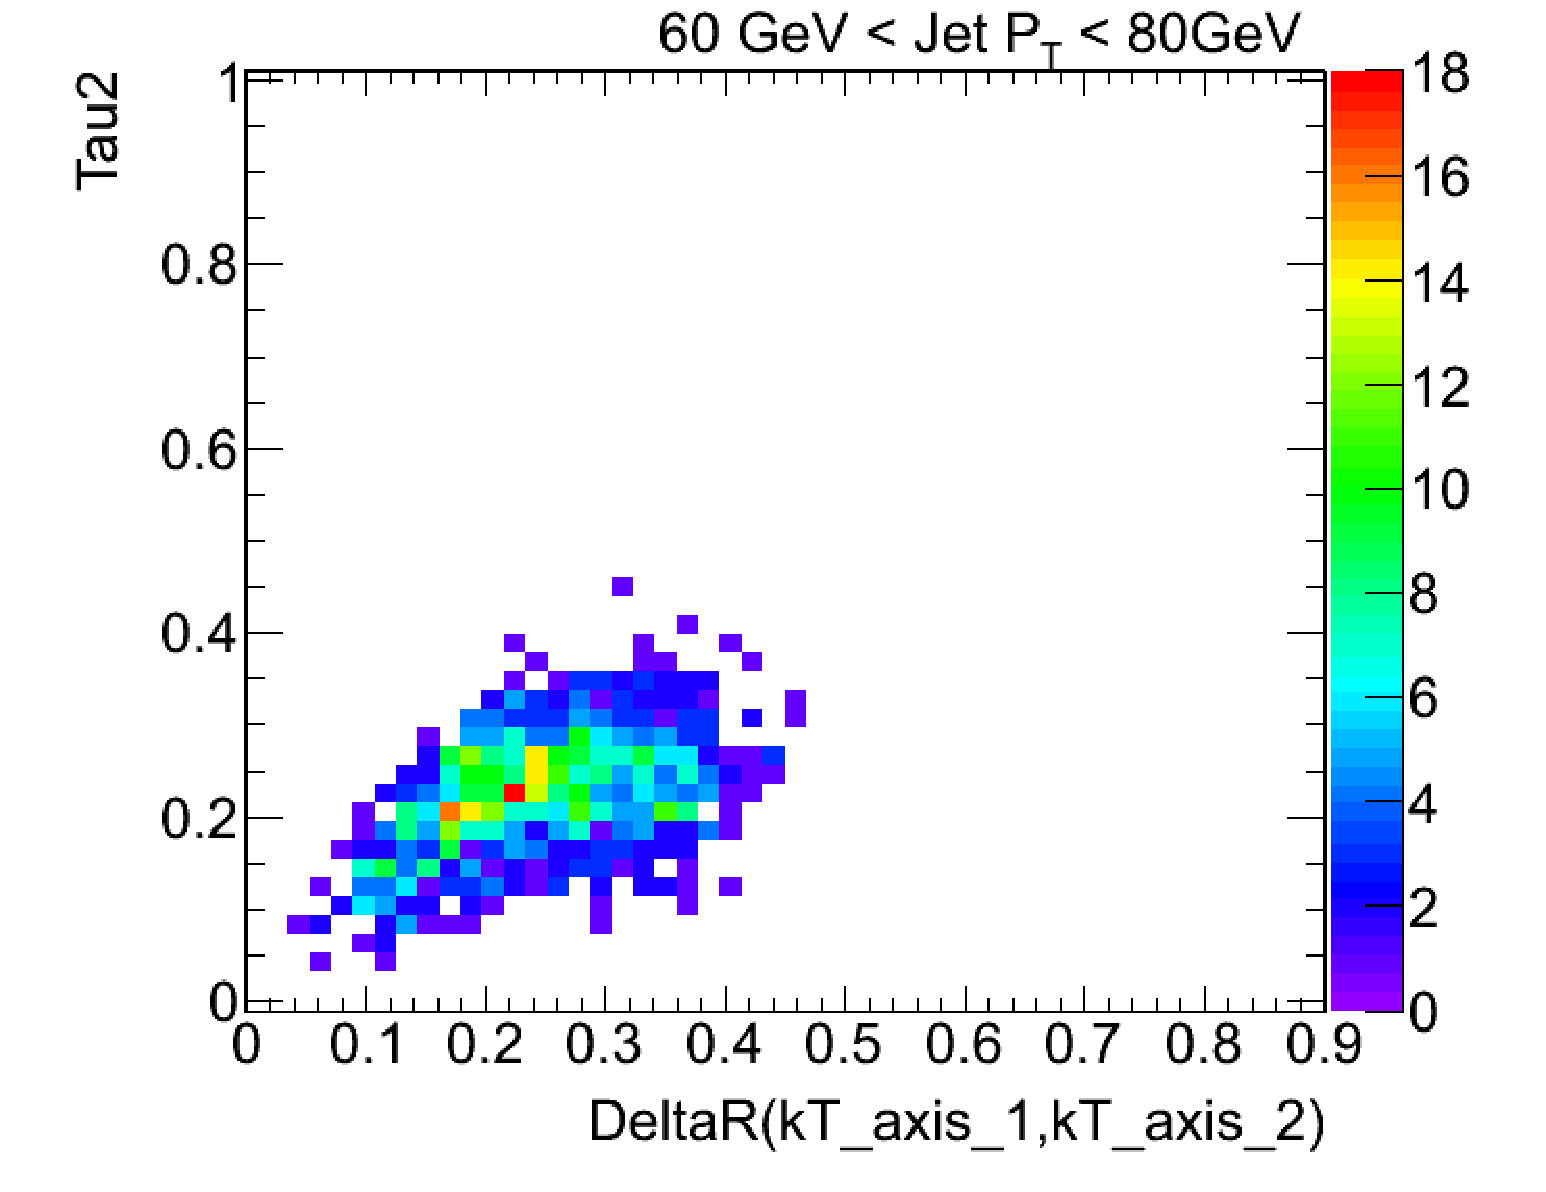
\includegraphics[width=0.49\textwidth]{FIGS/TEMPFigs/PythisStandalone/Antikt4/allparticles/Tau2DRkT2axesCorr_PT60_merged.pdf}
\caption{Correlation between $\tau_1$ (left) and $\tau_2$ (right) and the $\Delta R$ between the $k_T$ subjets in merged anti-$k_T$ 0.4 jets  between 60~GeV to 80~GeV. Jets were built using all stable particles.}
\label{fig:CorrTau1Tau2DRkt}
\end{figure}

%See email from Jesse Thaler
%Thu, Jun 2, 2011 at 7:43 PM
%subject:	 Re: N-subjettiness Code
%This is really fascinating, and it is starting to make some physical sense.  
For the single $b$-jets, $\tau_1$, $\tau_2$, and $\Delta R$ between the $k_T$ axes in the jet are all small which is expected for a pencil-like jet.  For the $b \bar{b}$-jets, these variables are all large, which is typical of a gluon jet.  But the correlations are really fascinating in merged $b$-jets.   $\tau_1$ and $\Delta R$ between the $k_T$ axes are nearly linearly related, which is expected if there are two hard lobes of energy.  But $\tau_2$ is almost independent of $\Delta R$ between the $k_T$ axes, meaning that regardless of where the axes are, the energy is uniformly distributed around them.
%So the question is whether you can make use of this.  tau1 and deltaR_12 are clearly useful variables, but they are also quite correlated.  tau2 appear to be uncorrelated with deltaR_12, but semi-correlated with tau_1.  By eye, the best discriminator for the R = 0.4 jets looks to be something like
%tau2 > (10 GeV/pT), deltaR_12 > (10 GeV/pT)
%or maybe
%(tau2 + deltaR_12) >  (20 GeV/pT).
%At this point, what would be helpful is to know whether your selection is really picking out g>bb jets or just picking up gluon jets in general.  For example, is the tau2 vs deltaR_12 non-correlation the same for generic gluon jets, or is it special to g>bb?  My intuition is that this must be a special feature of g>bb, since otherwise, it would be quite easy to separate gluon jets from quark jets...


%See this page for comparisons between g/b/bb from Max
%http://slac.stanford.edu/~swiatlow/gbb_plots/plots.html

%See mail from ariel 2 Jun 2011
%Quiza lo que este ocurriendo es que gbb fragmenta como normal (gluon) qcd, con mas splittings que b-jets (quarks) y sin la 2-body decay structura que estamos esperando.

%Date: Thu, 2 Jun 2011 20:37:57 +0200
%From: Ariel Schwartzman <sch@slac.stanford.edu>
%To: Maria Laura Gonzalez Silva <laugs@mail.cern.ch>
%Cc: Ricardo Piegaia <aia@df.uba.ar>, Laura <laugs@cern.ch>
%Subject: Re: N-subjettiness
% Muy interesante Laura.
% Tau1 aumenta con DRbb, como se espera, pues es como el jet width.
% Tau2 es casi flat con DR, lo que puede indicar dos cosas:
%  i) los kt-axis a los que se refiere Jesse no estan encontrando los dos B's
% ii) la contribucion de los tracks from B's es pequenia comparada con el resto de la fragmentacion, de modo de a que un gbb jet seria ungluon jet plus algunos soft displaced tracks on top.
% Te propngo algunos plots:
% 1) Jesse sugiere plotar el DR entre los dos kt axes para b y bb. Espero que quede claro en su codigo como axeder a esta variable...
% 2) Hace un 2D plot con la correlacion entre el DR entre los axes (1) y DR(B,B) para ver si esta definicion de axes corresponde a lo queesperamos.
%3) Vos habias mirado a DR(1,2) que es el DR entre los dos leading tracks. Podrias re-vivir estos estudios ahora con el generator study? Yhacer tambien el 2D plot de DR(1,2) vs DR(B,B)?
%4) Seria bueno repetir todas las input variables para pure gluon jets (esto lo sugeri en un mail el otro dia) para entender mejor cual es la diferencia entre gluones y gbb.
%5) Los dos blobs de energy que esperamos vienen de la hadronizacion de los B hadrons, mas que de la fragmentacion del gluon. Quiza estesea un key point que estamos ignorando. Yo estoy tentado a sugerir que calculemos las variables usando "displaced tracks" solamente. Ricardo, es posible ponerle un flag a las particulas que vienen de los B decays como para que Laura solo use estas particulas para calcular N-subjettiness?
%6) Event displays... son como la tool ideal para entender que esta pasando. Uno puede mirar event displays para jets con distinto DR(B,B), distuntos taus, etc... Fijate que todavia no tenemos una picture de cual es la shape de un gbb jet! Estuvimos asumiendo que uno espera 2 blobs de energy, pero no tenemos ningun plot que soporte esta idea en forma contundente.
%En todo caso, me parace perfecto tener esta discucion con Jesse. Ciertamente vamos a aprender mucho mas sobre gluon splitting...




%------------------------------------------------------------------------
\section{Kinematic differences between single and double $B$-hadron jets}\label{sec:gbbKine} %$b$- and merged $b\bar{b}$-jets}\label{sec:gbbKine}
%\section{Full ATLAS Monte Carlo Analysis}\label{sec:gbbKine}
%------------------------------------------------------------------------ 



The differences between genuine $b$-quark jets and $b \bar{b}$ jets are expected to arise from the two-subjet (two $B$-hadrons) substructure of merged jets.  They are thus expected, for the same jet $\pt$, to have higher track-multiplicity and be wider than single $b$-jets. Based on these characteristics %, the following properties were studied in simulated QCD samples of $b$-tagged jets using either calorimeter or track constituents:
simulated QCD samples of $b$-tagged jets were used to study the following properties, discussed in the next paragraphs, built from jet constituents either at calorimeter level (topological clusters) or tracks associated to the jet:

\begin{itemize}\addtolength{\itemsep}{-0.4\baselineskip}
\item
Jet multiplicity (number of constituents)
\item
Jet width, $\pt$ weighted %Track jet width ($\pt$ weighted)
\item 
Jet Mass
\item
Nr.\ of $k_t$ subjets %track-jets
\item
Maximum $\Delta R$ between pairs of constituents % (tracks)
\item
$\Delta R$ between 2 $k_t$ subjets within the $b$-jet
\item
$\tau_2$: 2-subjettiness 
\item
$\tau_2/\tau_1$
\item
$\Delta R$ of leading constituents %tracks
\item 
Eccentricity %(track & calo)
\end{itemize}


%Figures~\ref{fig:ntrksinglemerged} to~\ref{fig:tauratiosinglemerged} show the distributions and correlations of some of these variables in selected bins of $b$-tagged jet $\pt$. 

{ \em I. Jet track multiplicity}
\\[3mm]
This variable is defined as the number of tracks associated to the jet, it is simple to calculate and carries important information of the jet inner structure. Figure~\ref{fig:ntrksinglemerged} shows the distribution of the observable for single and merged $b$-jets.  It was observed that merged $b$-jets contain on average around two more tracks than single $b$-jets at low jet $\pt$, with a larger difference at higher $\pt$ values. The jet track multiplicity corresponds to tracks with $\pt$ above 1 GeV, satisfying the quality cuts described in section~\ref{sec:EventSelection}. The effect of using a minimum track $\pt$ of 0.5 GeV was also examined. This was motivated by the fact that it could lead to an improvement in discrimination if it captured more information about the fragmentation process.  On ther other hand, a lower minimum track $\pt$ can make the method more sensitive to pile-up with the addition of soft tracks incorrectly associated to the jets.  What it was observed is that reducing the $\pt$ cut only widens the distributions without increasing the separation between single and merged jets. 
\begin{figure}[tp]
\centering
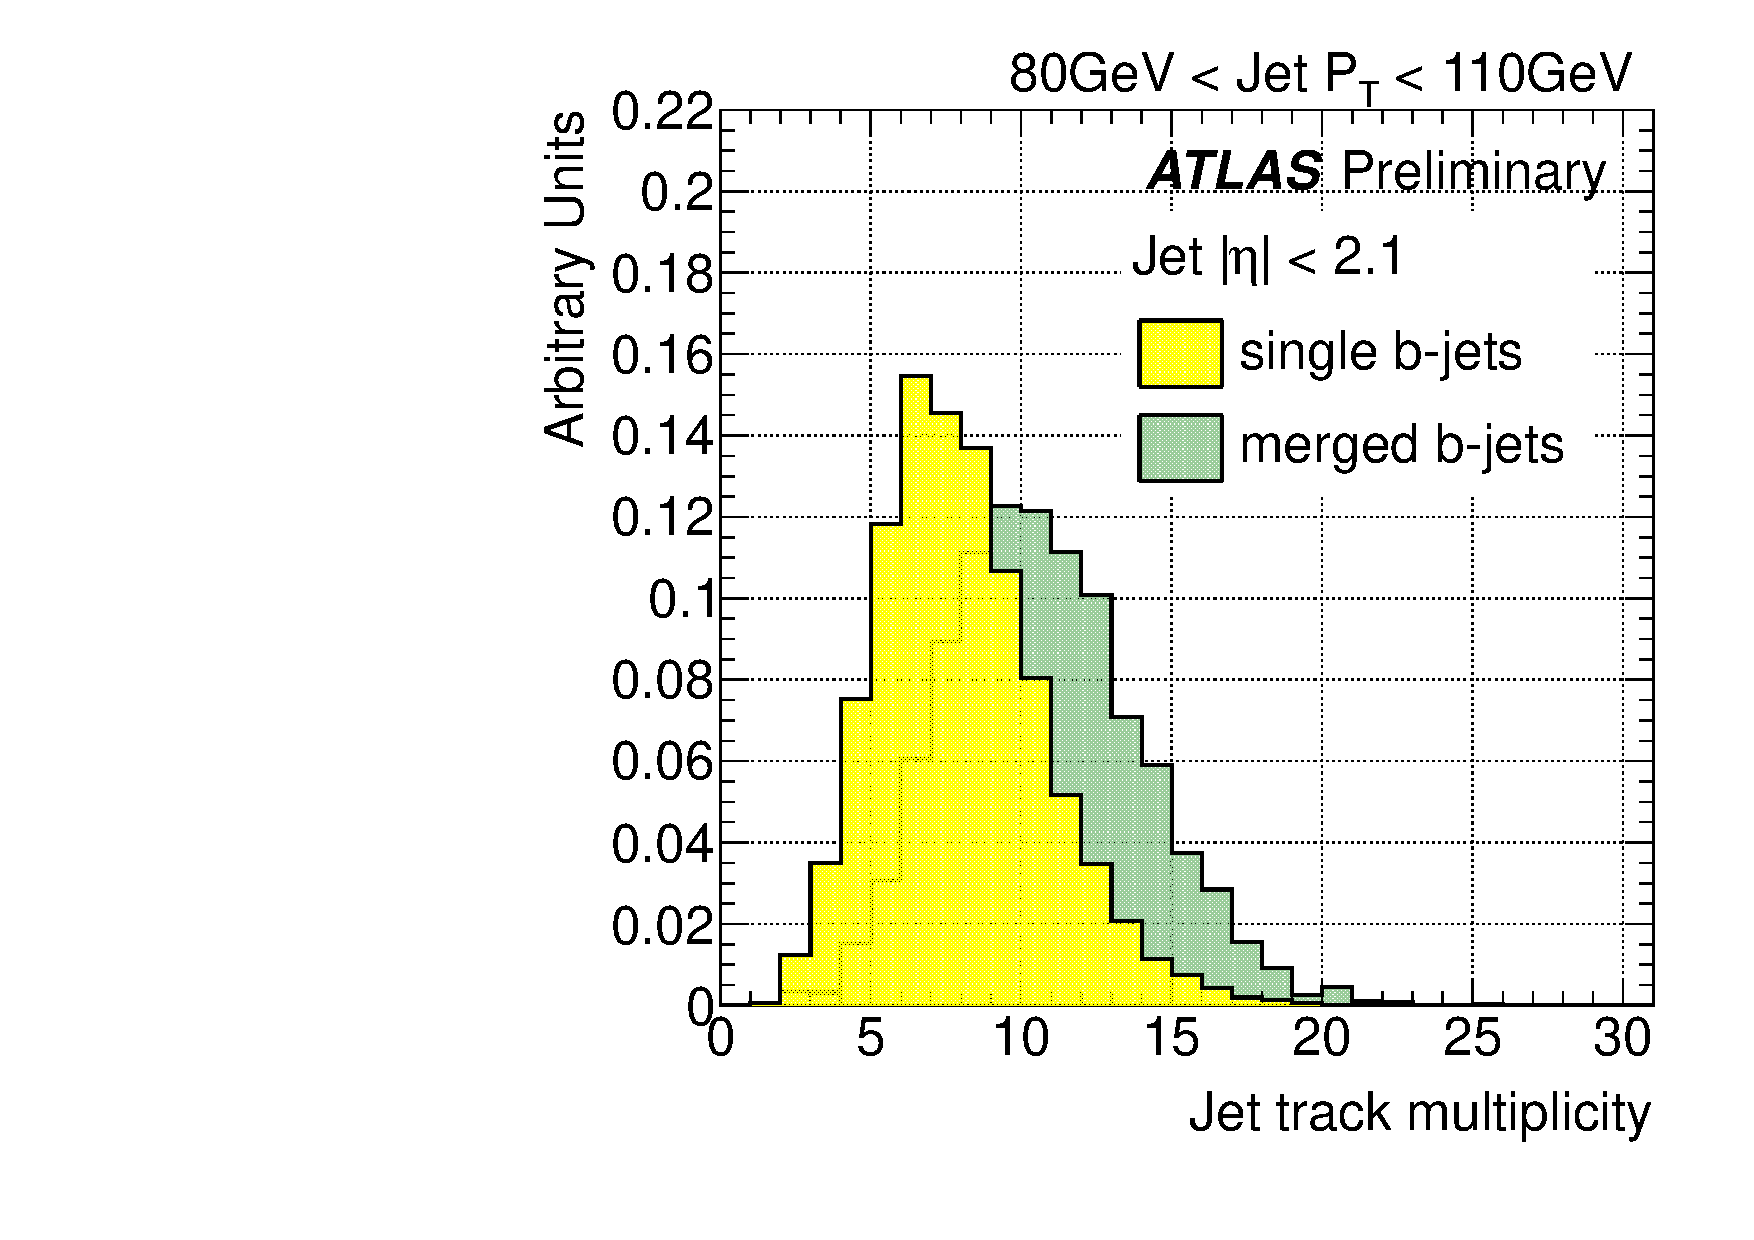
\includegraphics[width=0.49\textwidth]{FIGS/VarsSingleMerged/Ntrk080.pdf}
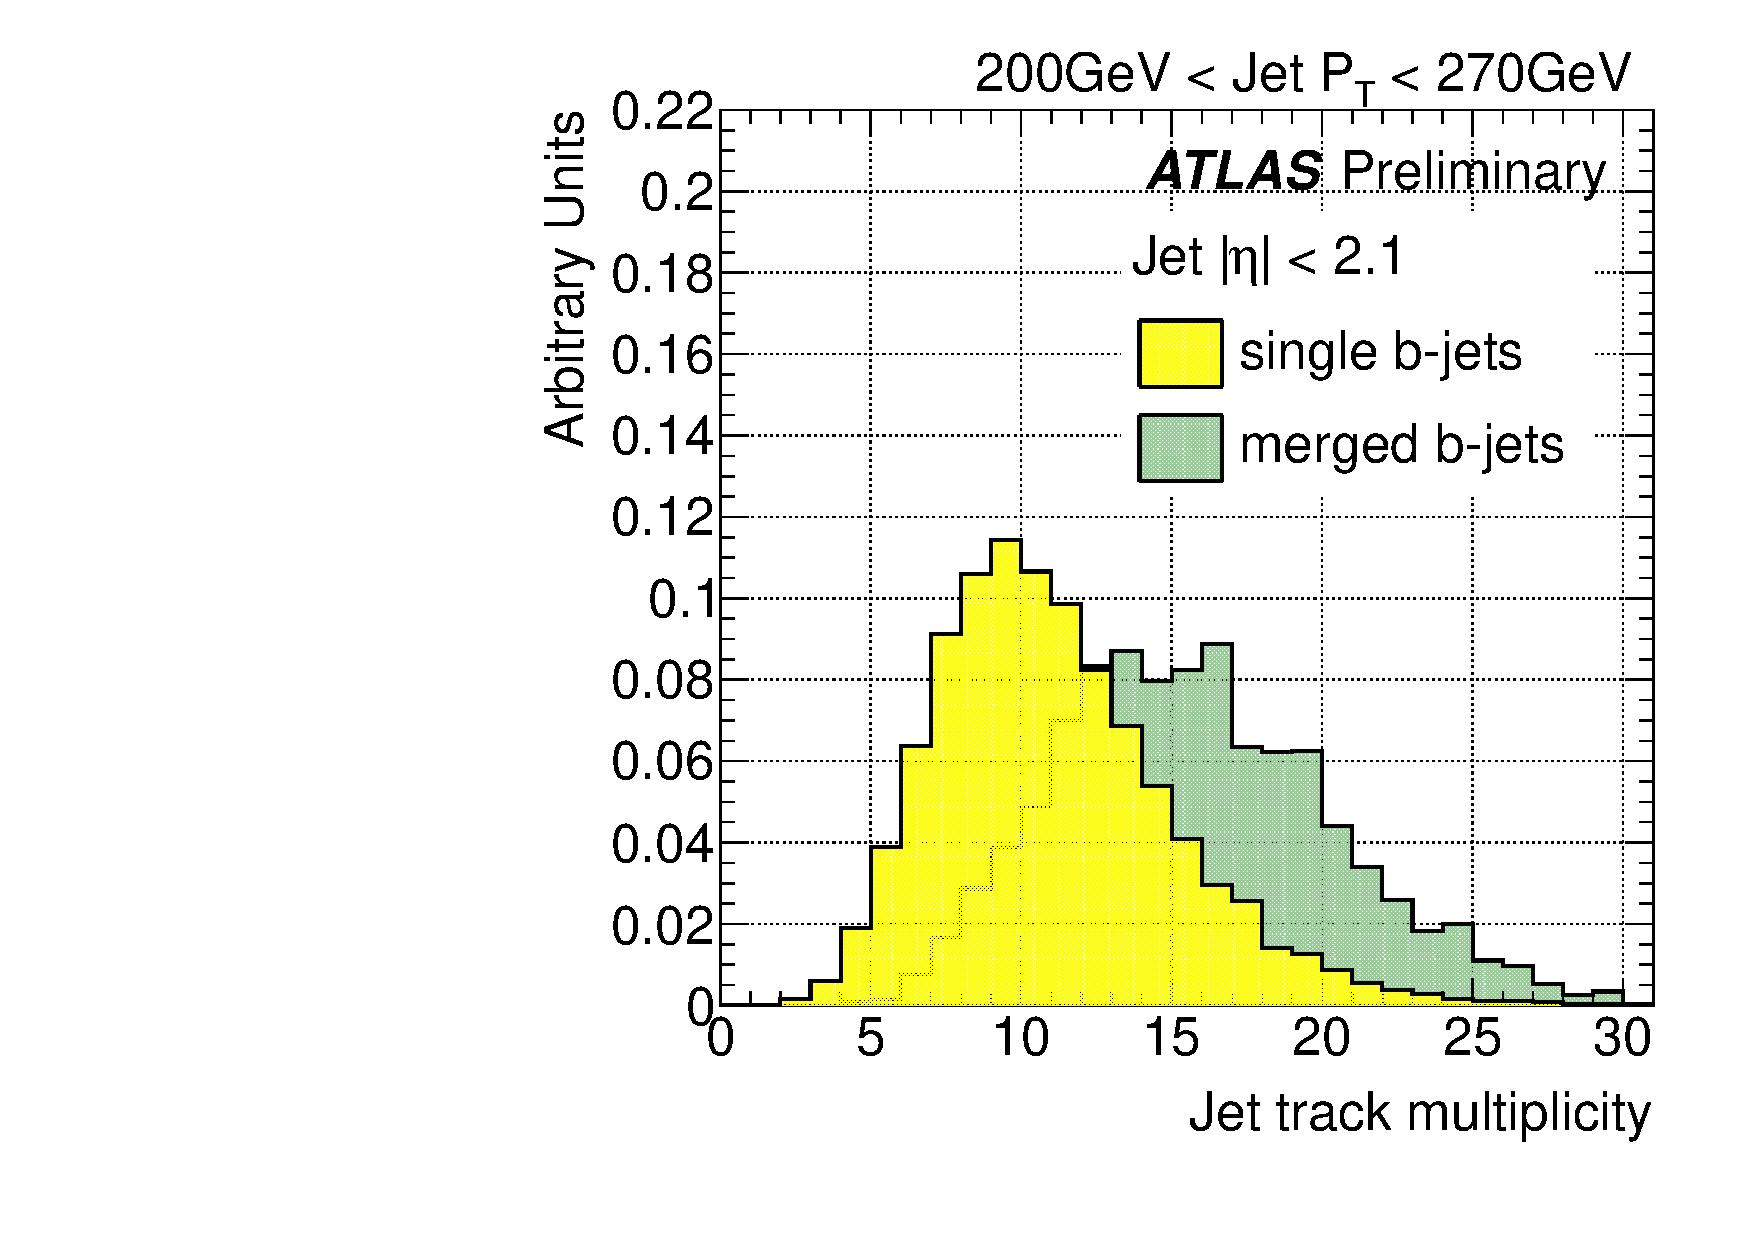
\includegraphics[width=0.49\textwidth]{FIGS/VarsSingleMerged/Ntrk200.pdf}
\caption{Distribution of the track multiplicity in jets for single and merged $b$-jets between 80~GeV to 110~GeV (left) and 200~GeV to 270~GeV (right).}
\label{fig:ntrksinglemerged}
\end{figure}

{ \em II. Jet width}
\\[3mm]
 The jet width was computed as the $\pt$ weighted average of the $\Delta R$ distance between the associated constituent (``$const$'') and the jet axis:
\begin{equation} 
\mbox{ {\it Jet width}} = \frac{\sum_{i=1}^N \pt^{const_i} \,\Delta R (const_i,jet) }{\sum_{i=1}^N \pt^{const_i} }
\label{eqn:trackjetwidth}
\end{equation} 
where $N$ is the total number of calorimeter or track constituents.

Figure~\ref{fig:trkwidthsinglemerged} shows the distribution for the Track-jet width. As expected, merged $b$-jets are wider than single $b$-jets. In Fig.~\ref{fig:ntrktrkwidthsinglemerged} the correlation between the track-jet width and the jet track multiplicity is shown for single and merged $b$-jets. These two variables alone provide a good discrimination for tagging $b \bar{b}$ jets.

The calorimeter jet width ( using topological clusters) gives also good separation. However, this variable is more sensitive to the amount of pile-up in the event than its track-based counterpart. In Fig.~\ref{fig:calowidthpileup} the distributions of calorimeter width for single and merged $b$-jets  can be seen for events with low and high Number of Primary Vertices (NPV), in a low $\pt$ region where the effect of pile-up is more important. In Fig.~\ref{fig:trkwidthpileup} the same distributions are shown for the track-jet width. Calorimeter jet width varies %significatively
with NPV and due to this behavior the track-based version is more suitable as a more robust discriminator. For similar reasons, the jet topological cluster multiplicity and the jet mass were discarded as discriminating variables.
\\[3mm]

\begin{figure}[tp]
\centering
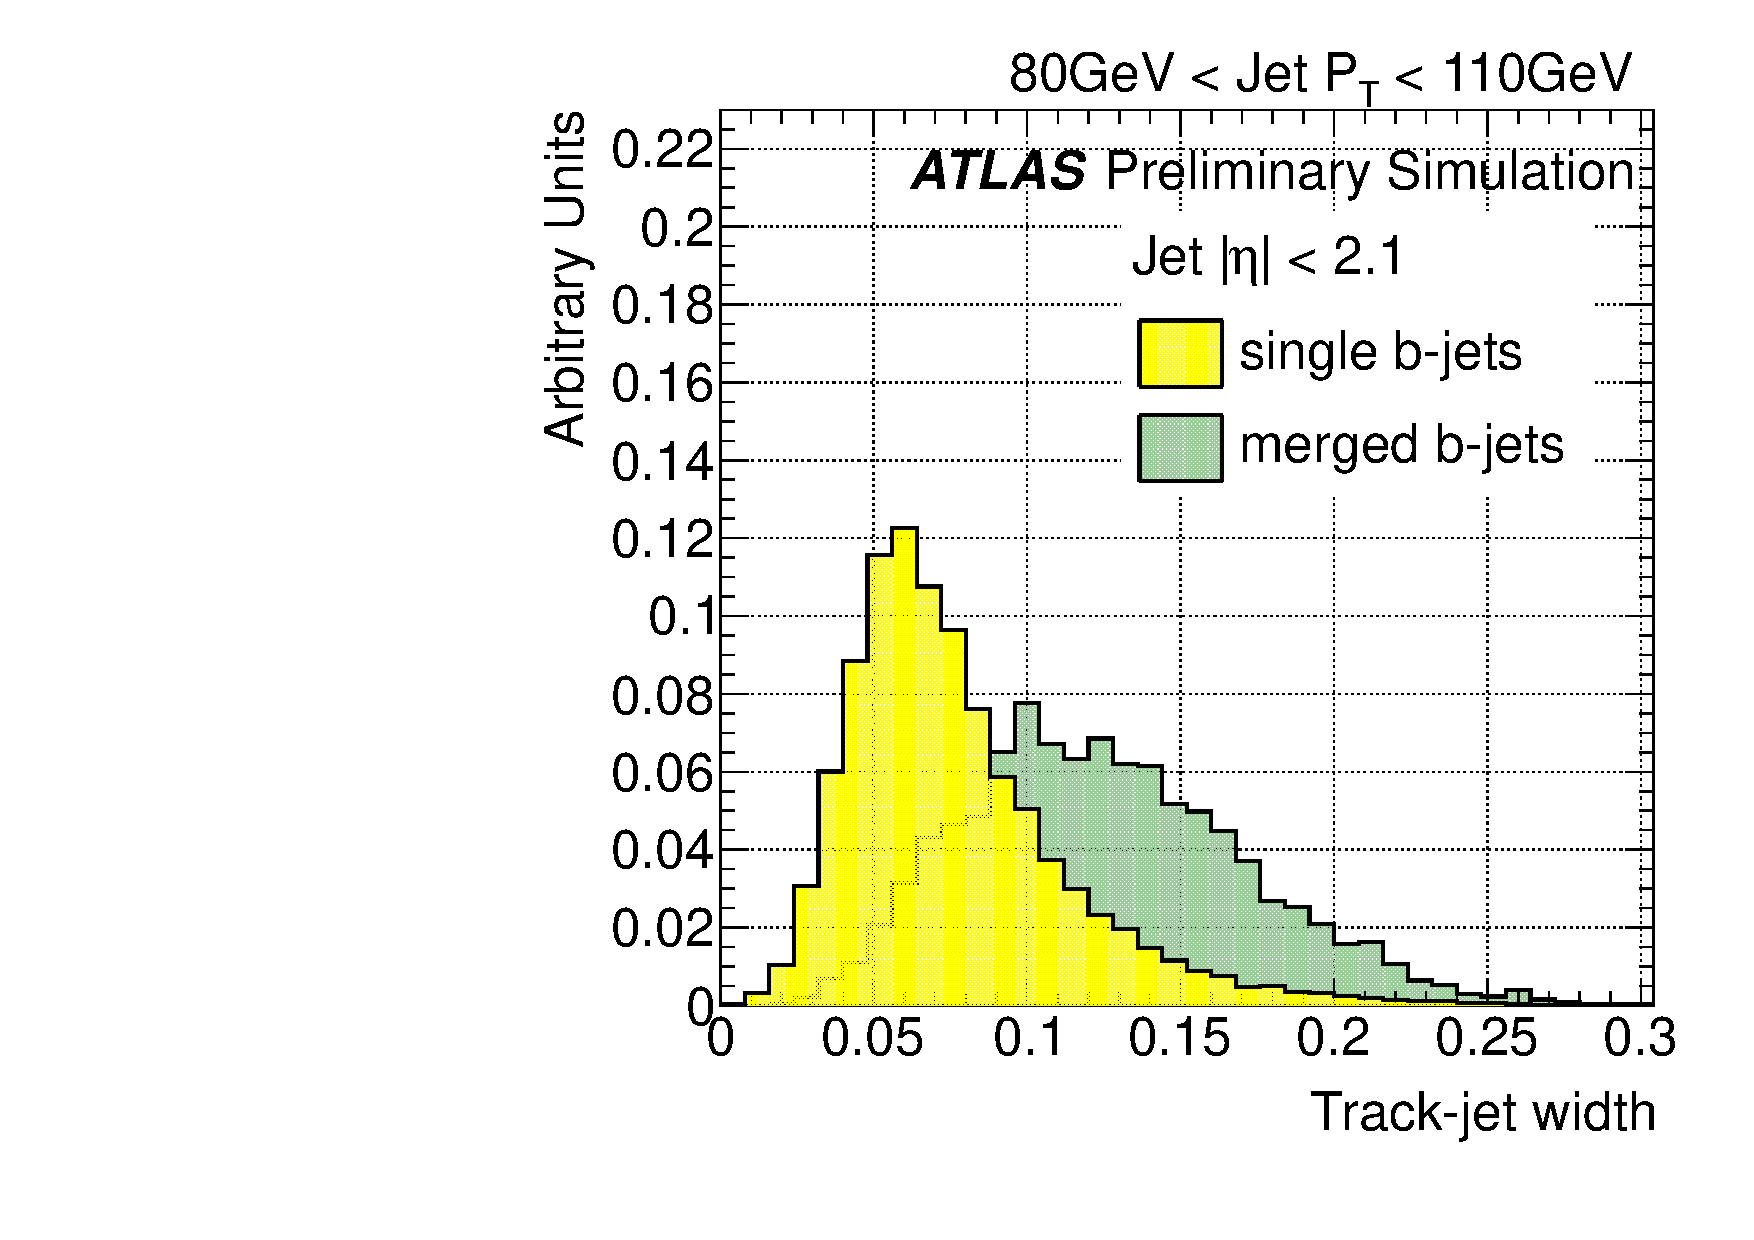
\includegraphics[width=0.49\textwidth]{FIGS/VarsSingleMerged/trkWidth080.pdf}
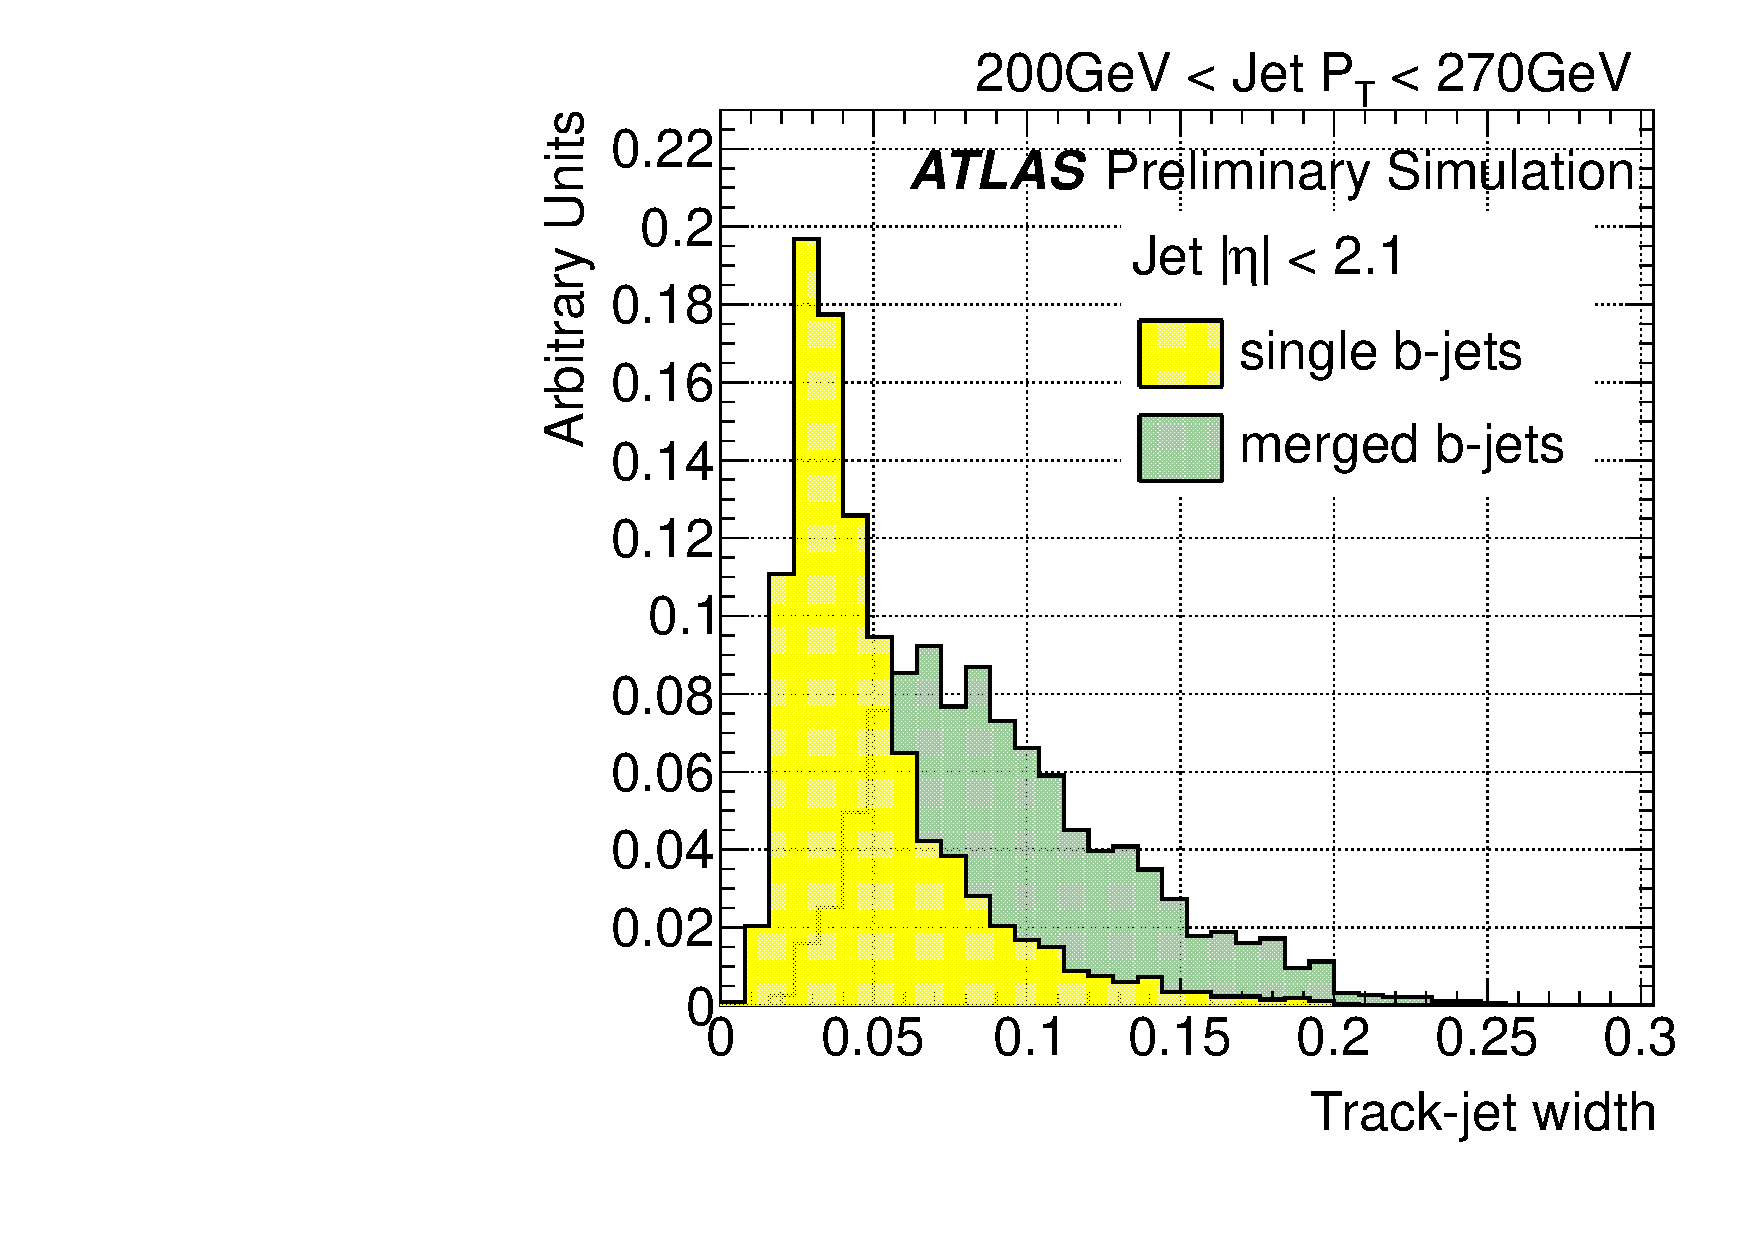
\includegraphics[width=0.49\textwidth]{FIGS/VarsSingleMerged/trkWidth200.pdf}
\caption{Distribution of track-jet width in jets for single and merged $b$-jets between 80~GeV to 110~GeV (left) and 200~GeV to 270~GeV (right).}
\label{fig:trkwidthsinglemerged}
\end{figure}

\begin{figure}[tp]
\centering
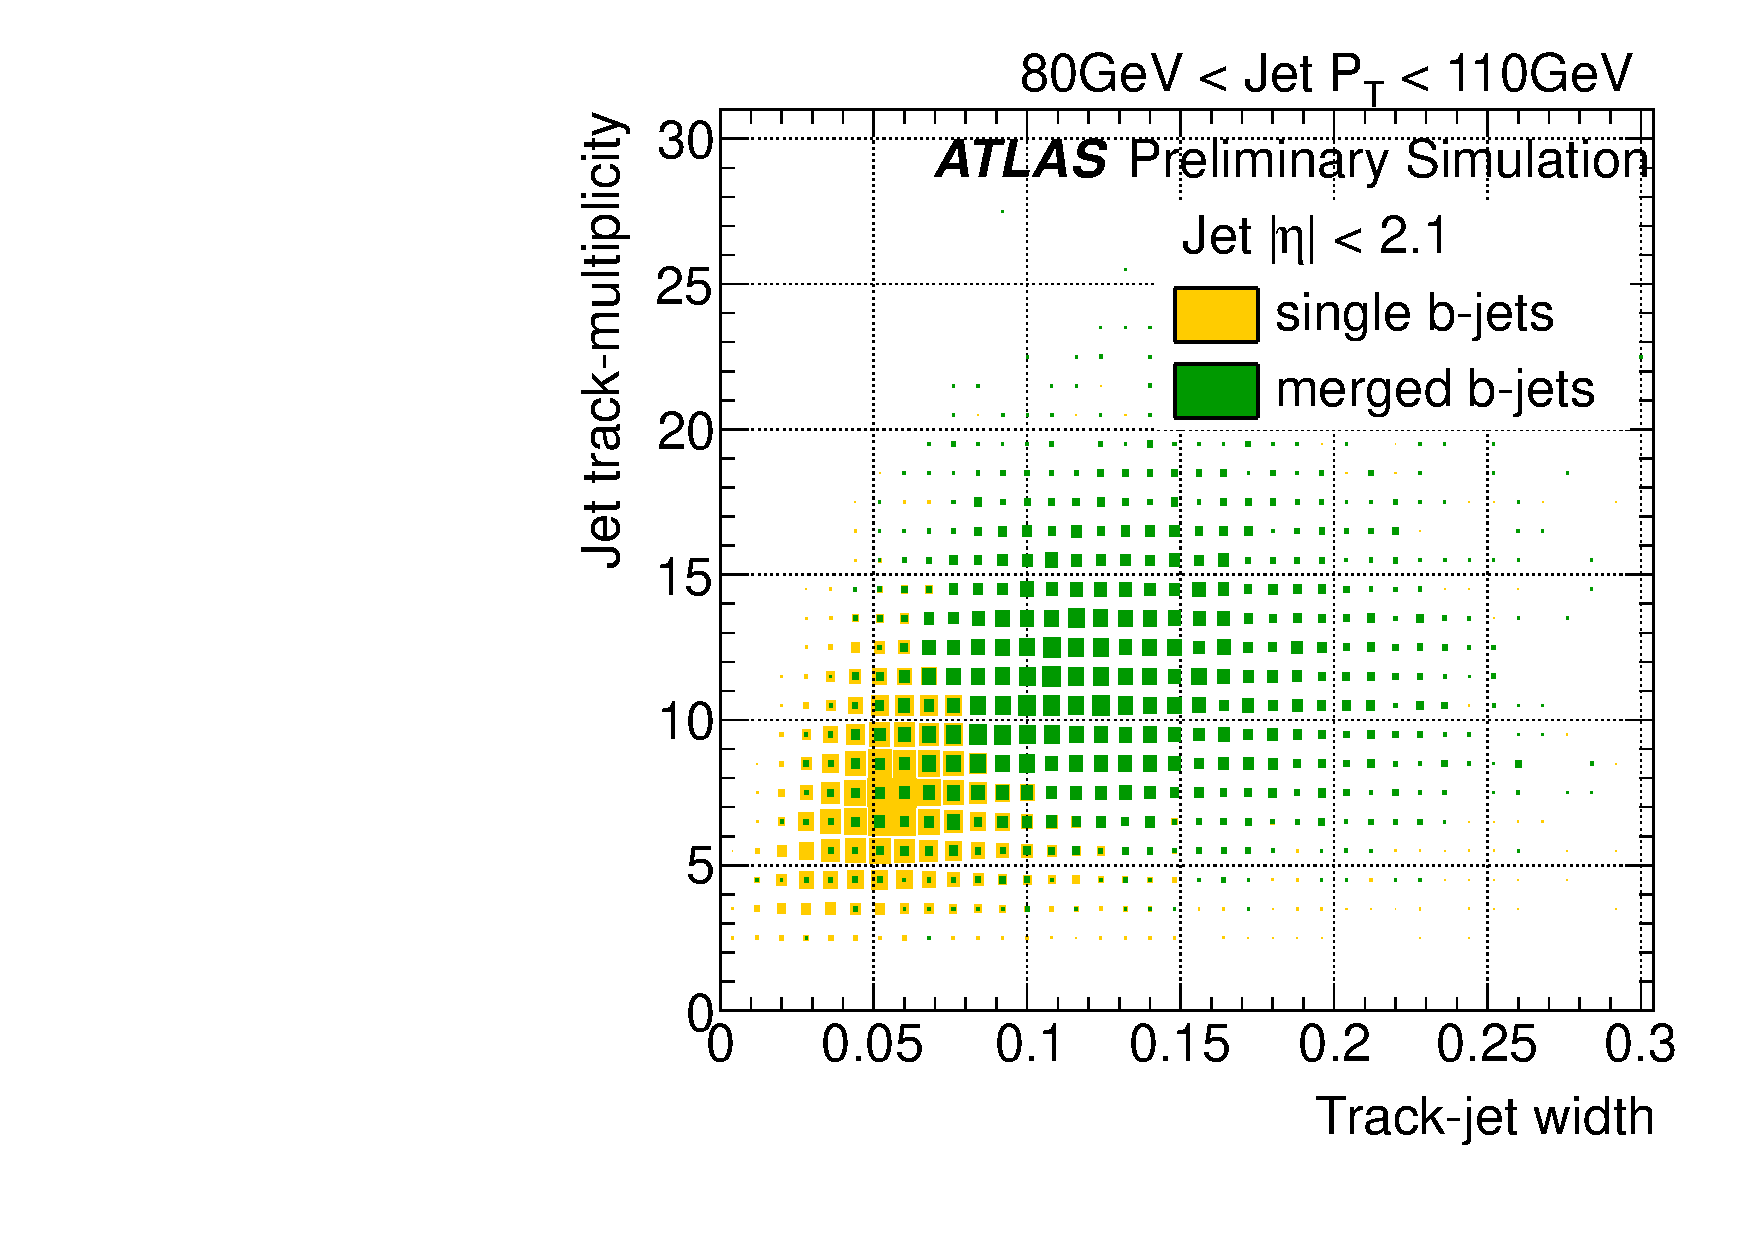
\includegraphics[width=0.49\textwidth]{FIGS/VarsSingleMerged/NtrktrkWidth080.pdf}
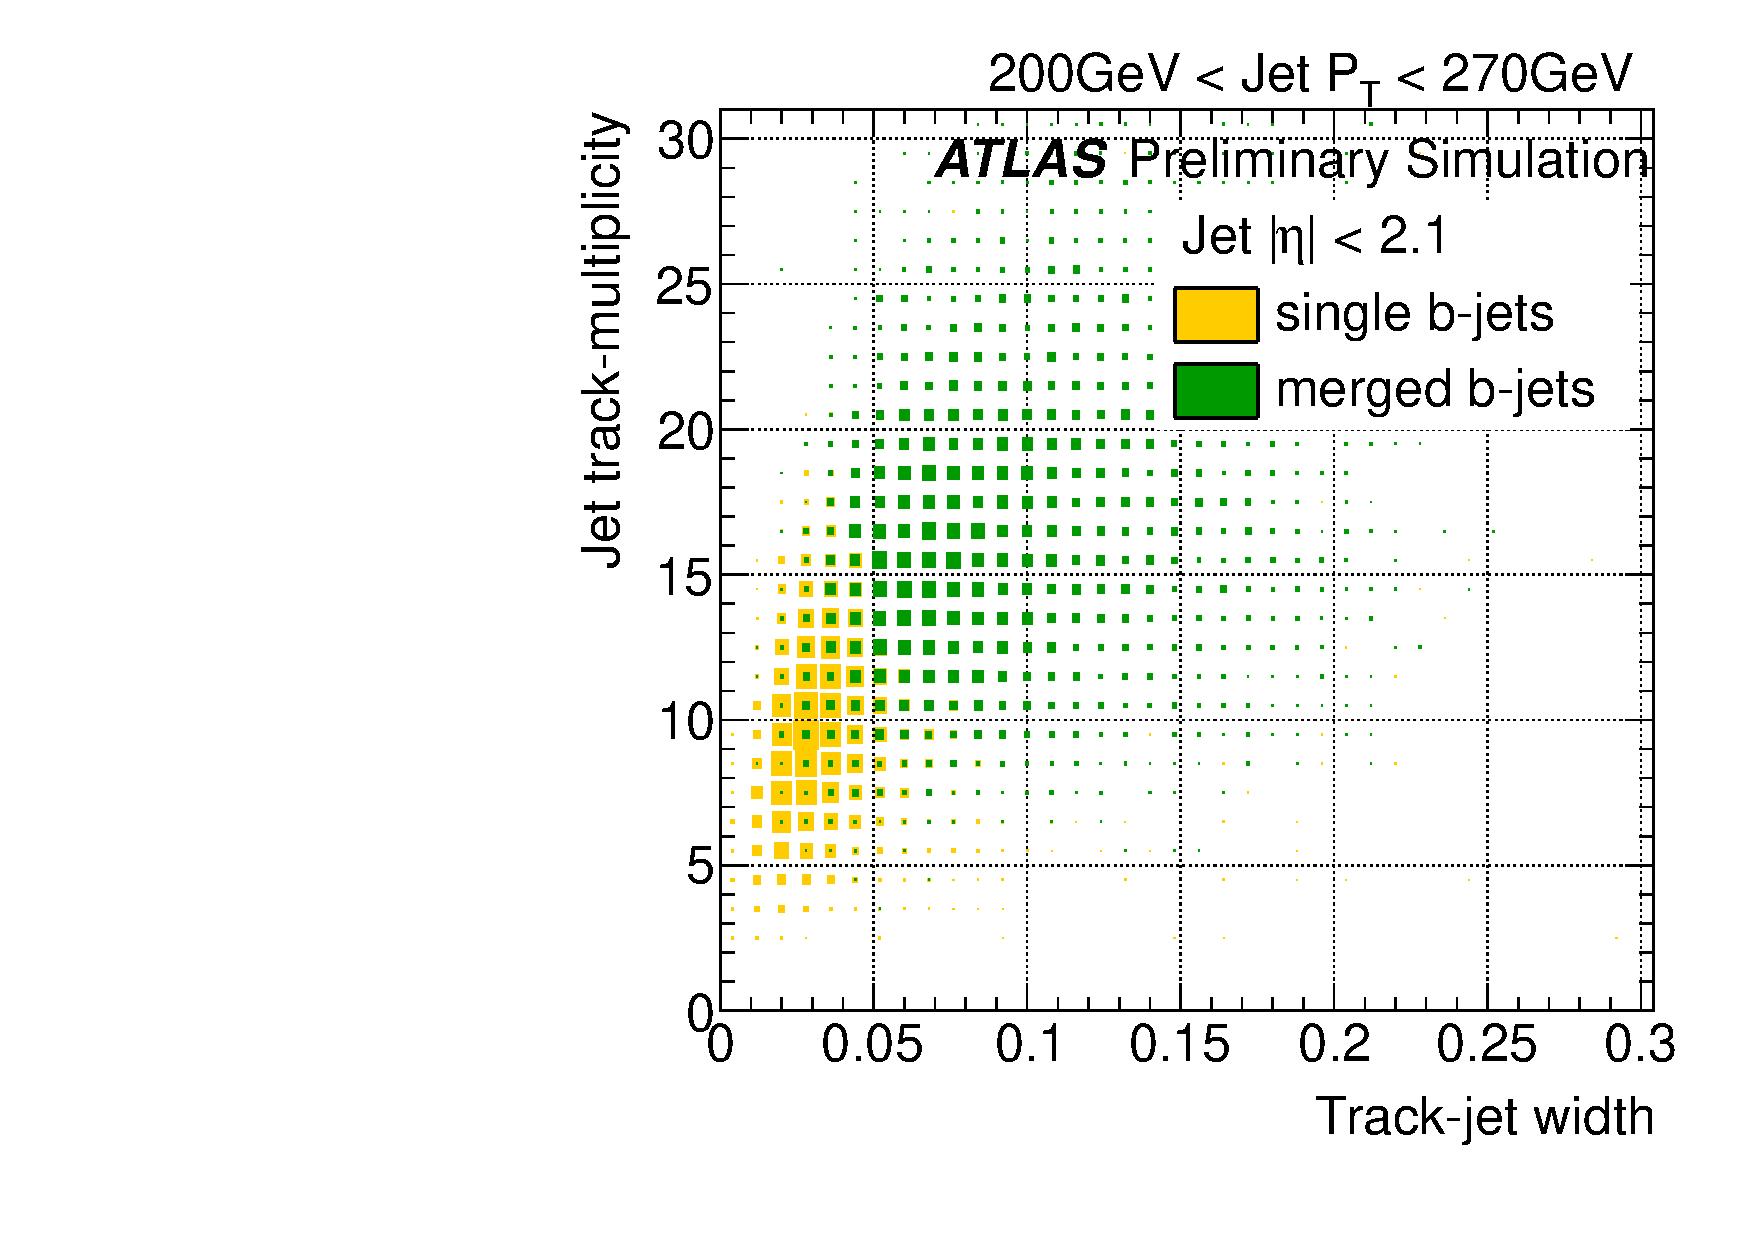
\includegraphics[width=0.49\textwidth]{FIGS/VarsSingleMerged/NtrktrkWidth200.pdf}
\caption{Correlation between jet track multiplicity and track-jet width for single and merged $b$-jets between 80~GeV to 110~GeV (left) and 200~GeV to 270~GeV (right).}
\label{fig:ntrktrkwidthsinglemerged}
\end{figure}

\begin{figure}[tp]
\centering
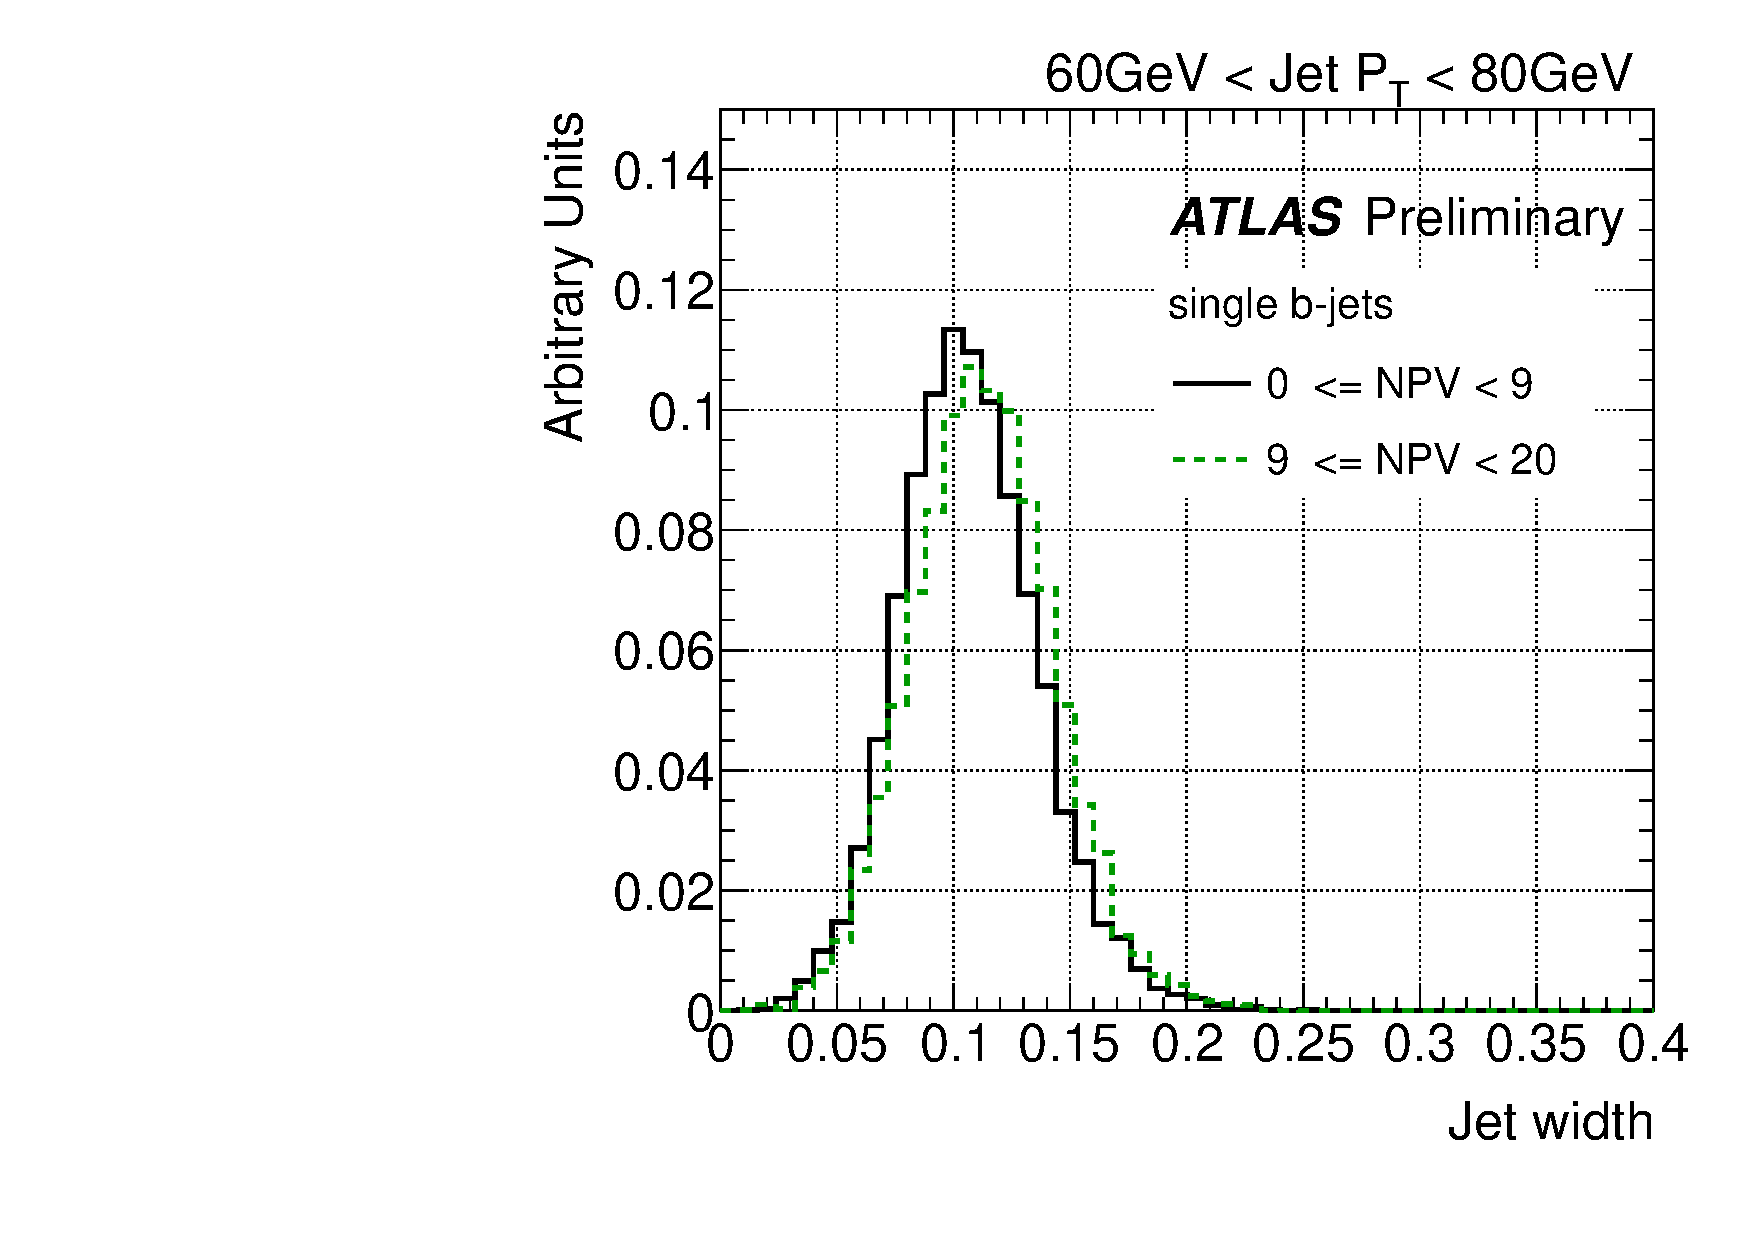
\includegraphics[width=0.49\textwidth]{FIGS/systematics/Widthsingle_060.pdf}
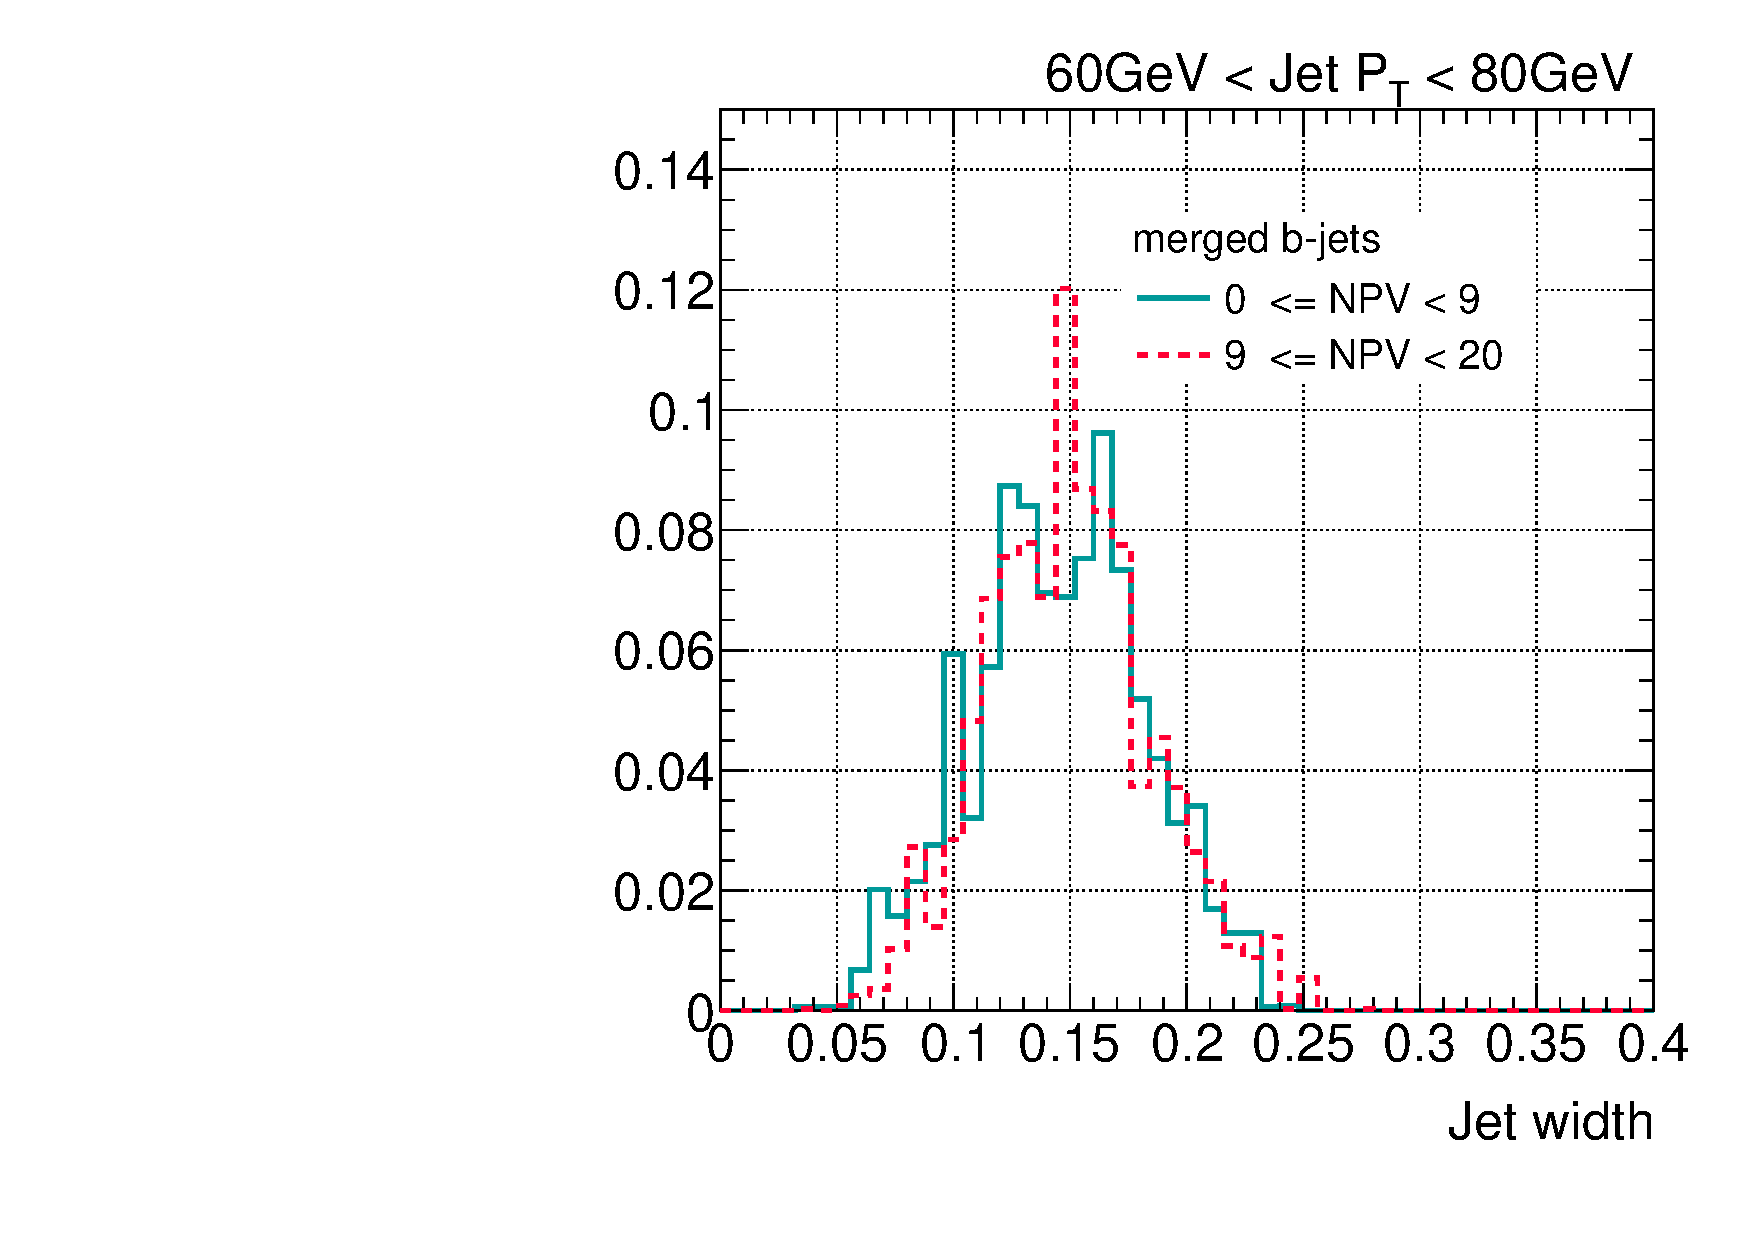
\includegraphics[width=0.49\textwidth]{FIGS/systematics/Widthmerged_060.pdf}
\caption{Distribution of calorimeter jet width (using topological clusters) for single (left) and merged (right) $b$-jets in two bins of Number of Primary Vertices for jets between 60~GeV to 80~GeV.}
\label{fig:calowidthpileup}
\end{figure}


\begin{figure}[tp]
\centering
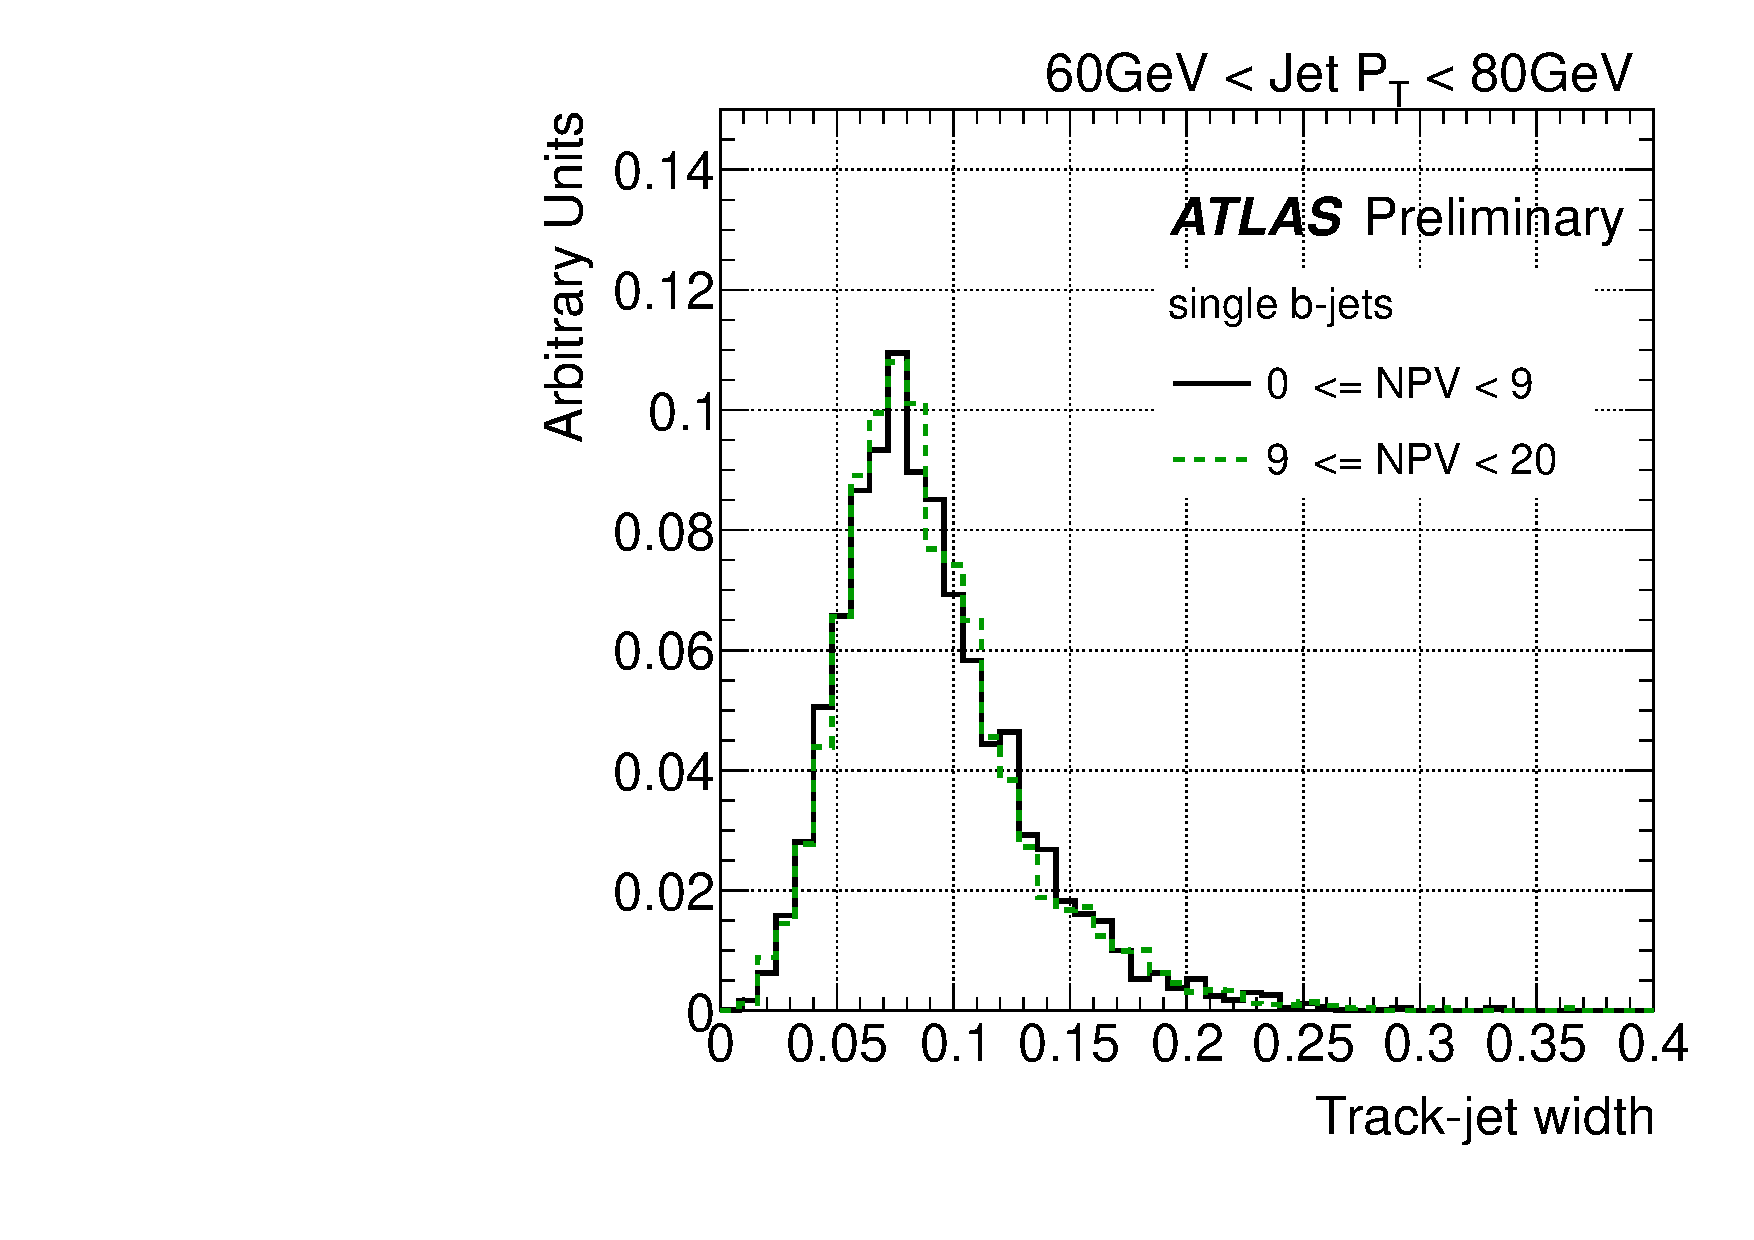
\includegraphics[width=0.49\textwidth]{FIGS/systematics/trkWidthsingle_060.pdf}
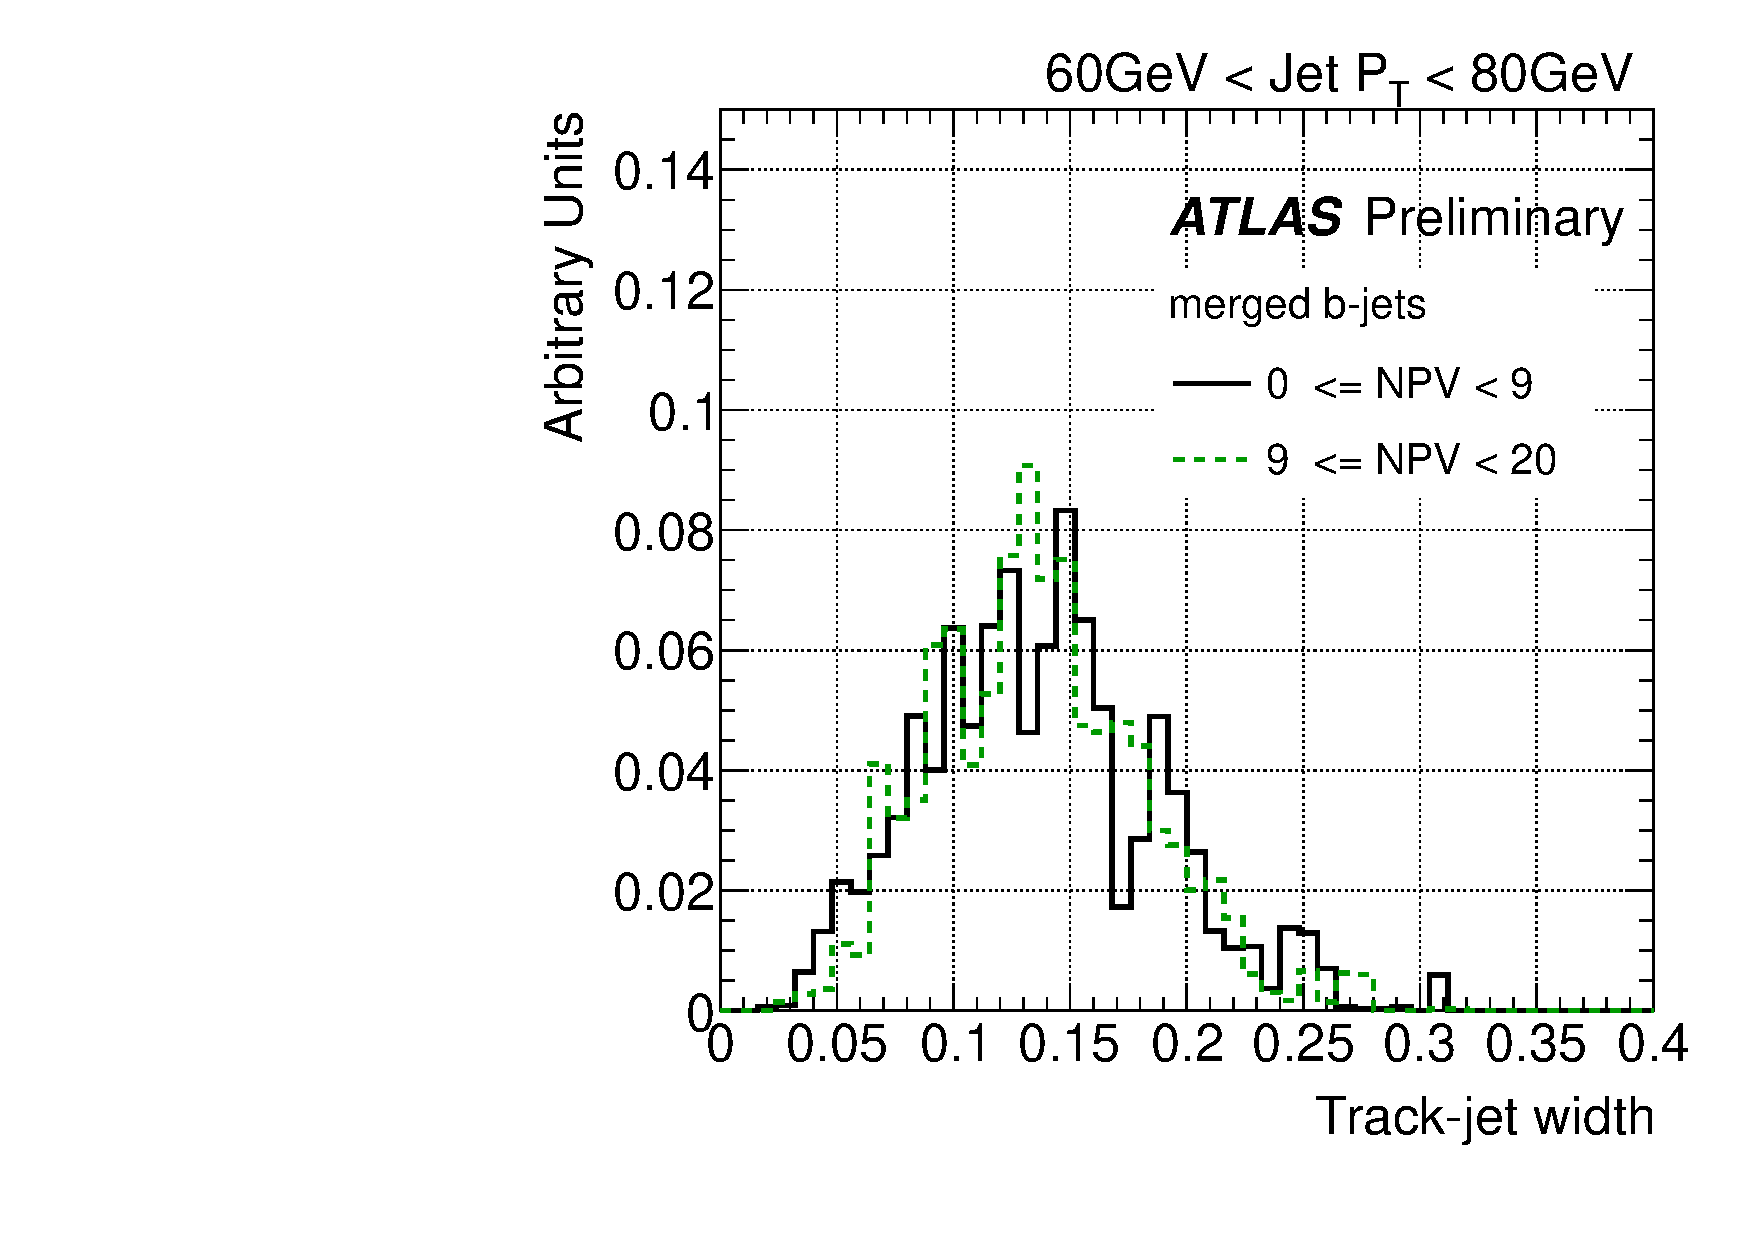
\includegraphics[width=0.49\textwidth]{FIGS/systematics/trkWidthmerged_060.pdf}
\caption{Distribution of track-jet width for single (left) and merged (right) $b$-jets in two bins of Number of Primary Vertices for jets between 60~GeV to 80~GeV.}
\label{fig:trkwidthpileup}
\end{figure}



{ \em III. Maximum $\Delta R$ between track pairs}
\\[3mm]
Figure~\ref{fig:drmaxsinglemerged} shows the distribution of the maximum $\Delta R$ between track pairs in the jets (Max$\{\Delta R(trk,trk)\}$). Merged $b$-jets show significantly higher values for this variable over a broad range of jet $\pt$. The distinct characteristic of this variable is that the separation between single $b$-jets and merged does not depend on jet $\pt$. In spite of its good discrimination power, we have looked for alternatives to Max$\{\Delta R(trk,trk)\}$ as it is not an infrared safe observable and is sensitive to soft tracks originating from pile-up. 
\\[3mm]

\begin{figure}[tp]
\centering
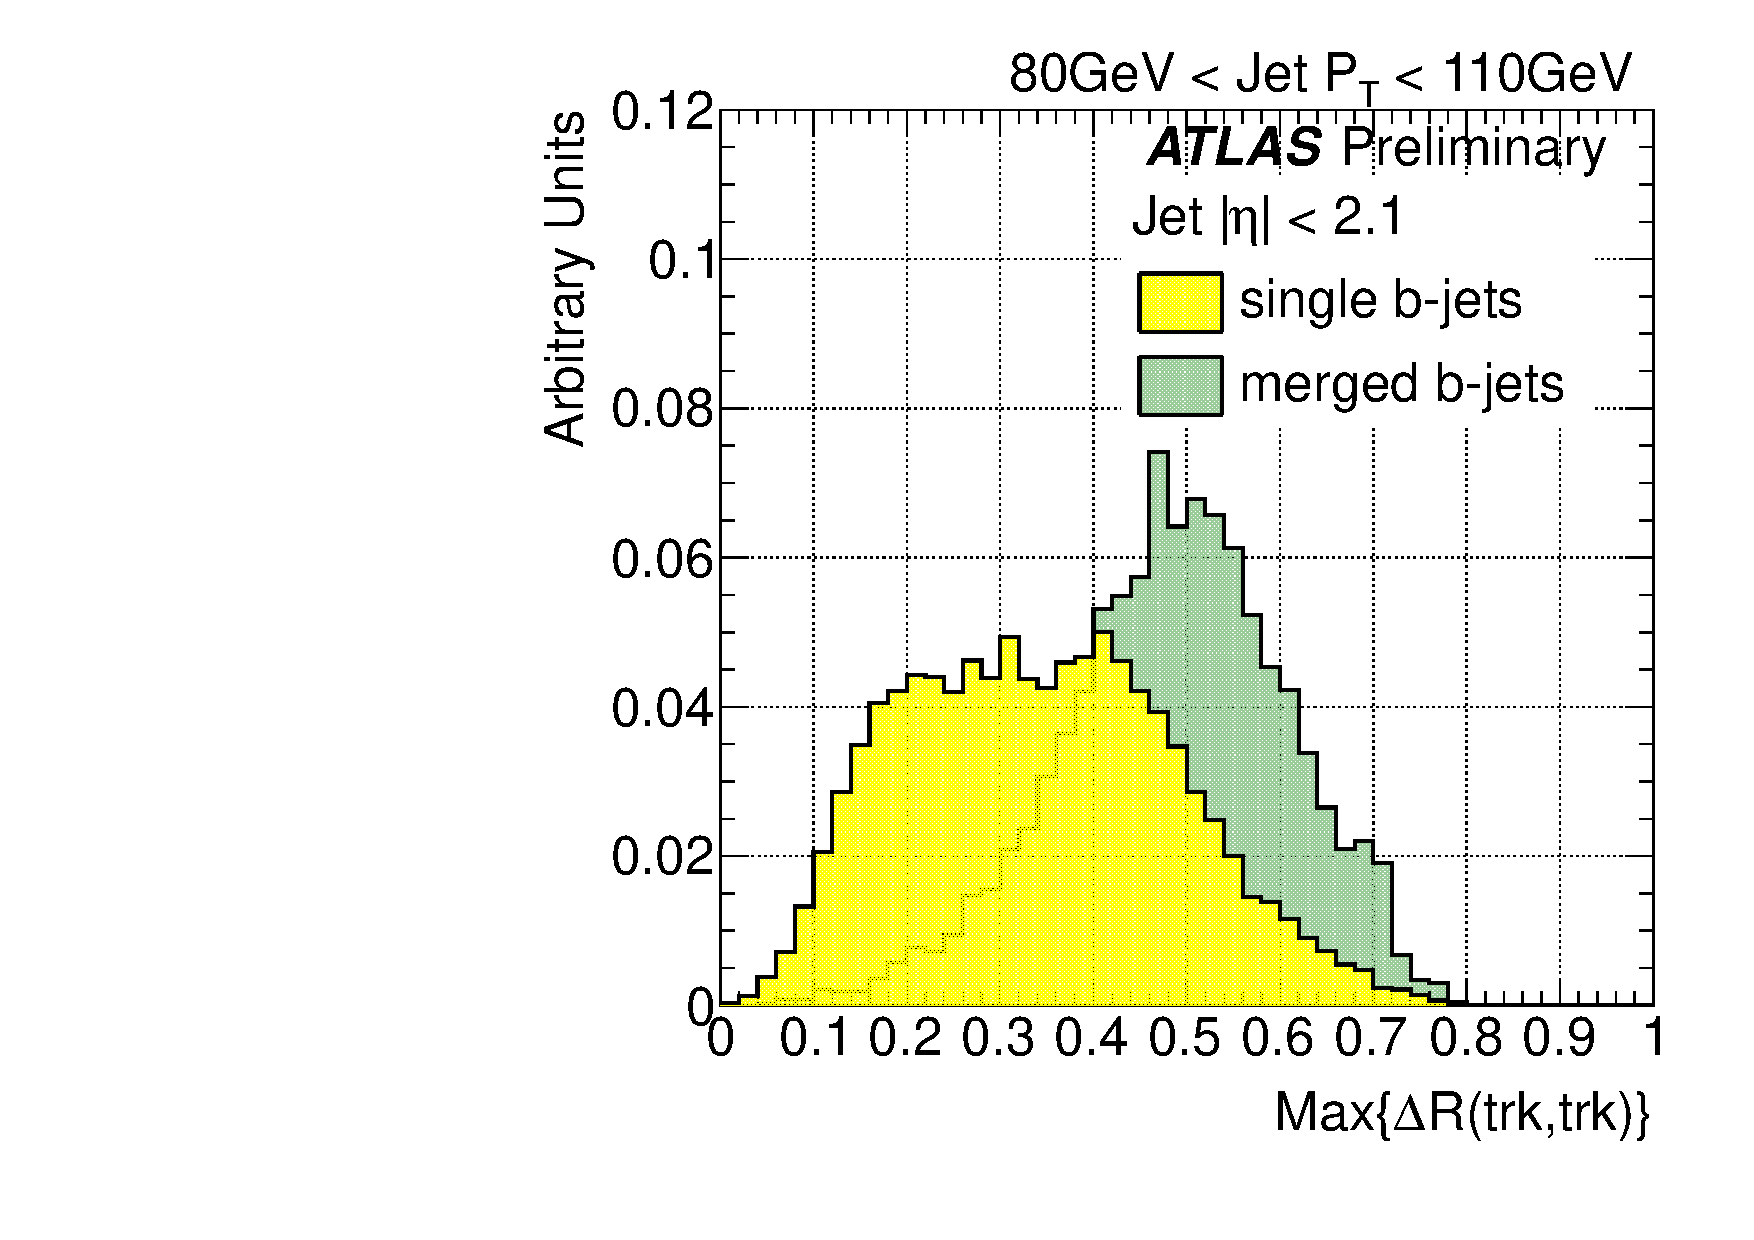
\includegraphics[width=0.49\textwidth]{FIGS/VarsSingleMerged/drmax080.pdf}
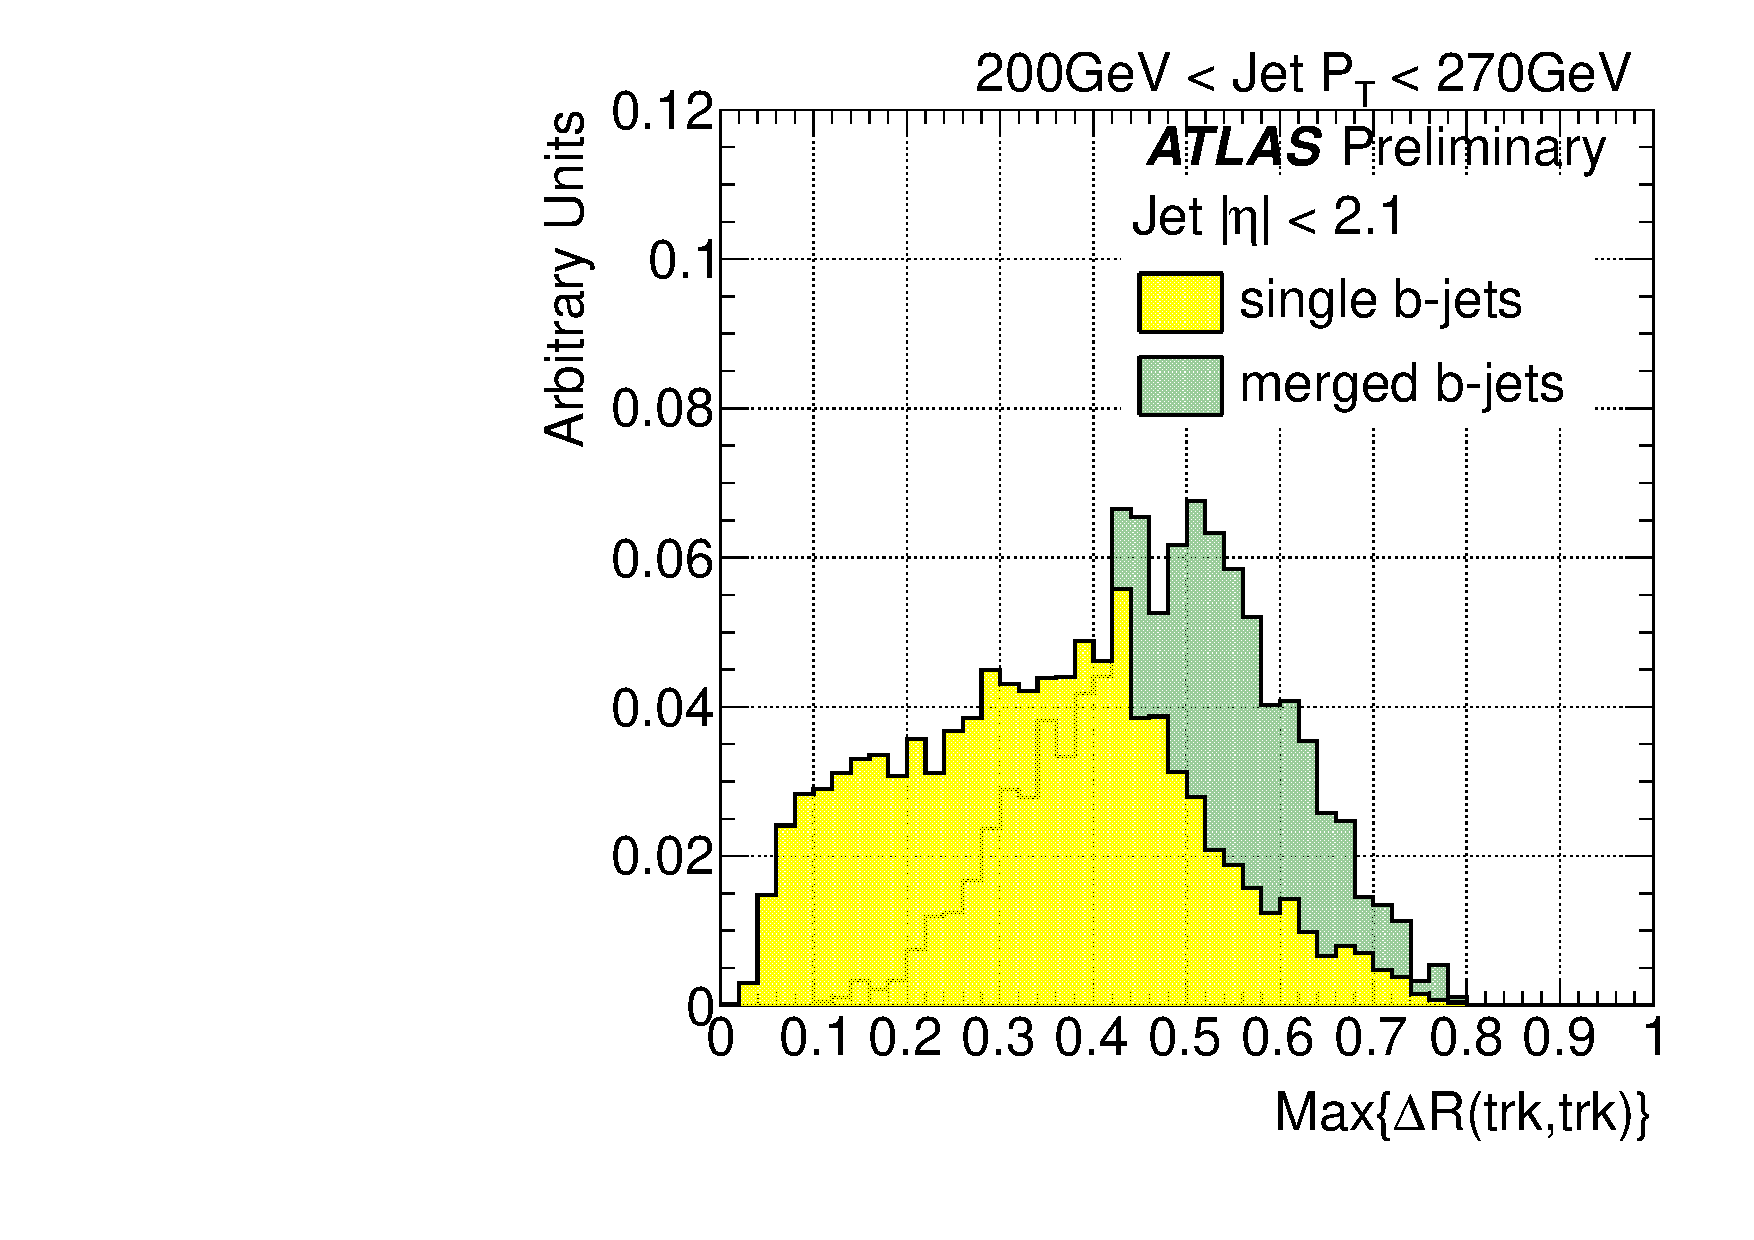
\includegraphics[width=0.49\textwidth]{FIGS/VarsSingleMerged/drmax200.pdf}
\caption{Distribution of the maximum $\Delta R$ between pairs of tracks in jets for single and merged $b$-jets between 80~GeV to 110~GeV (left) and 200~GeV to 270~GeV (right).}
\label{fig:drmaxsinglemerged}
\end{figure}


{ \em IV. $\Delta R$ between the axes of two $k_t$ subjets}
\\[3mm]
The distribution of the $\Delta R$ between the axes of the two exclusive $k_t$ subjets in the jet is shown in Fig.~\ref{fig:drktsinglemerged} for single and merged $b$-jets. In order to build this variable the $k_t$ algorithm~\cite{kt1} is applied to all the tracks associated to the jet using a large $k_t$  distance parameter to ensure that all of them get clustered. The clustering is stopped once it reaches exactly two jets. We observe that this variable also provides good separation, with the advantage of infrared safeness and insensitivity to pile-up. % revealing the two-prong substructure of merged $b$-jets.
\\[3mm]

\begin{figure}[tp]
\centering
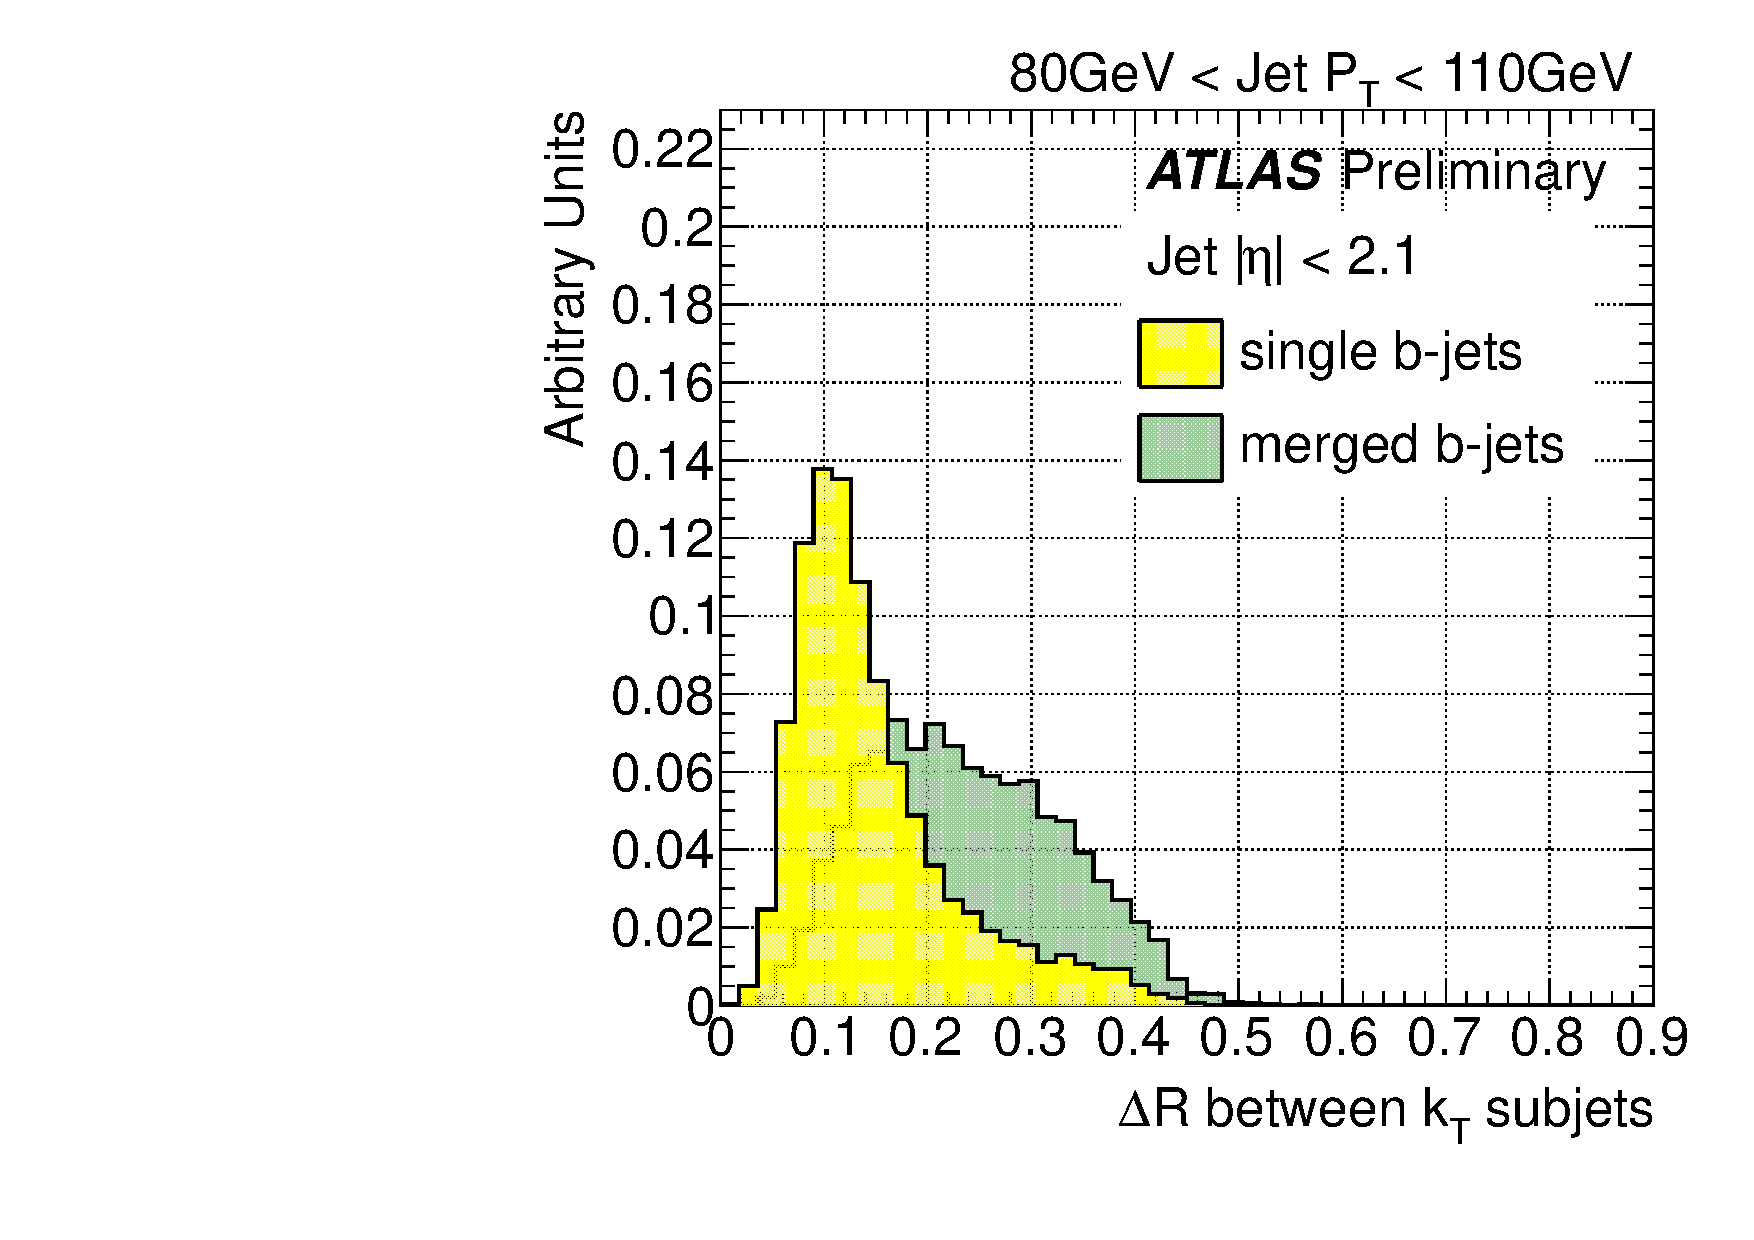
\includegraphics[width=0.49\textwidth]{FIGS/VarsSingleMerged/DRkt2axes080.pdf}
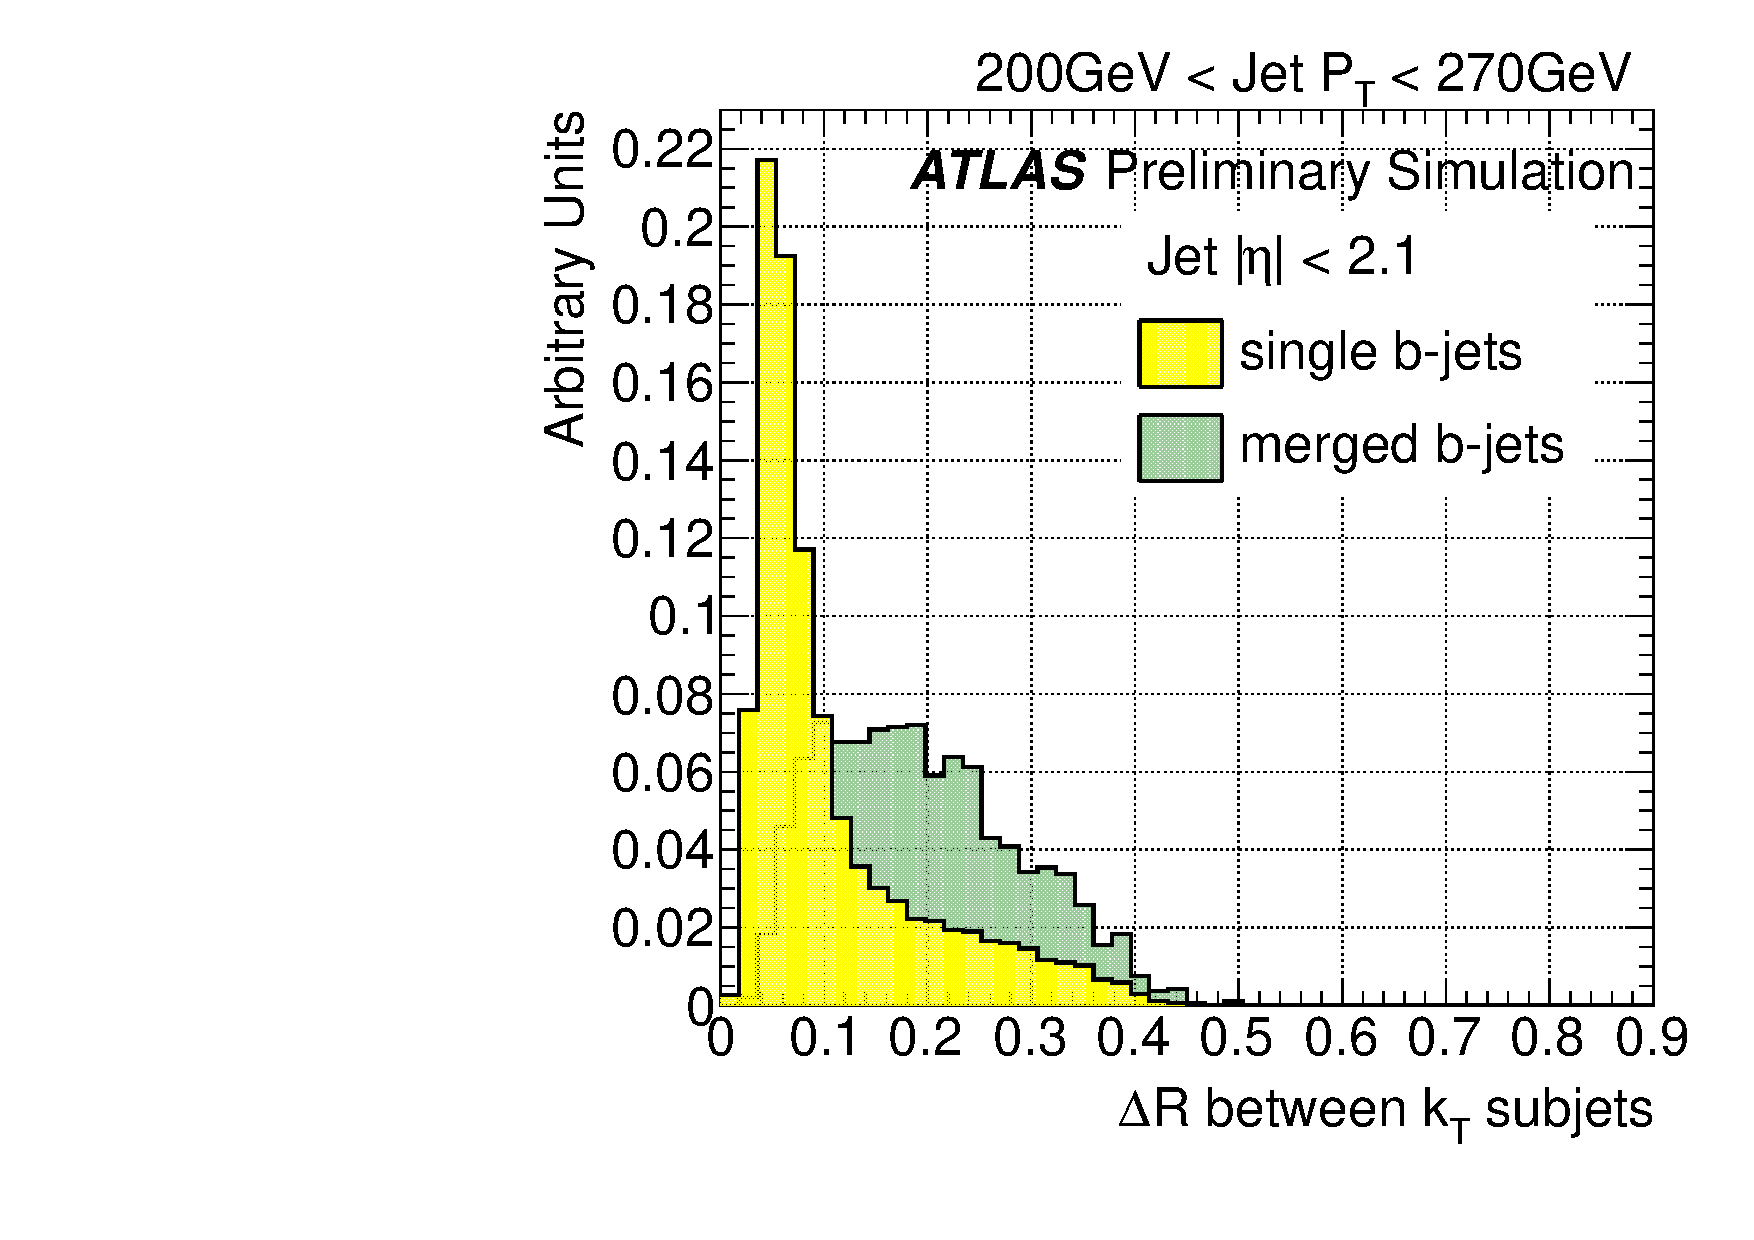
\includegraphics[width=0.49\textwidth]{FIGS/VarsSingleMerged/DRkt2axes200.pdf}
\caption{Distribution of the $\Delta R$ between the axes of the two $k_t$ subjets in the jet for single and merged $b$-jets between 80~GeV to 110~GeV (left) and 200~GeV to 270~GeV (right).}
\label{fig:drktsinglemerged}
\end{figure}


{ \em V. $N$-subjettiness variables}
\\[3mm]

$N$-subjettiness variables, as described in Ref.~\cite{nsubjettiness}, were originally designed to identify boosted objects, like electroweak bosons and top quarks, decaying into collimated shower of hadrons which a standard jet algorithm would reconstruct as single jets. It is defined as:
\begin{equation} 
\tau_N = \frac{1}{\sum_k {\pt}_k\,R_0} \sum_k {\pt}_k \min \{ \Delta R_{S_1,k},\,\Delta R_{S_2,k},...,\,\Delta R_{S_N,k} \}
\end{equation} 
where $R_0$ is the jet radius used in the jet clustering algorithm and the sum runs over the constituents of the jet. To avoid dependence on pile-up we consider the track-based $n$-subjettiness, where the sum 
 is over the tracks in the $b$-tagged jet. $\Delta R_{S_j,k} $ is the distance in the rapidity-azimuth plane between the axis of subjet $j$ and constituent track $k$. This jet shape variable quantifies to what degree a jet can be regarded as composed of $N$ subjets. For instance, a jet with a two pronged structure, with all tracks clustered along two directions, is expected to have a smaller $\tau_2$ value than a jet with tracks uniformly distributed in $\eta-\phi$ space.

Plots of $ \tau_2$ are shown in Fig.~\ref{fig:tau2singlemerged}. In spite of its expected 2-prong substructure, merged $b$-jets have higher values of $ \tau_2$ than single $b$-jets. The explanation of this behavior can be found in Fig.~\ref{fig:tau2trkwidthsinglemerged}, where its correlation with  track-jet width ($\sim \tau_1$) is shown for single and merged $b$-jets. The two variables are highly correlated and for this reason wider jets  have a larger $ \tau_2$. This suggests to switch from an absolute to a width-normalized
$\tau_2$. Fig.~\ref{fig:tauratiosinglemerged} thus shows the distributions of $\tau_2/\tau_1$. This ratio is often used but, although as expected somewhat larger values are obtained for single than for merged $b$-jets, specially at high $\pt$, we decided not to use this variable as it offers only marginal discrimination. 
\\[3mm]

\begin{figure}[tp]
\centering
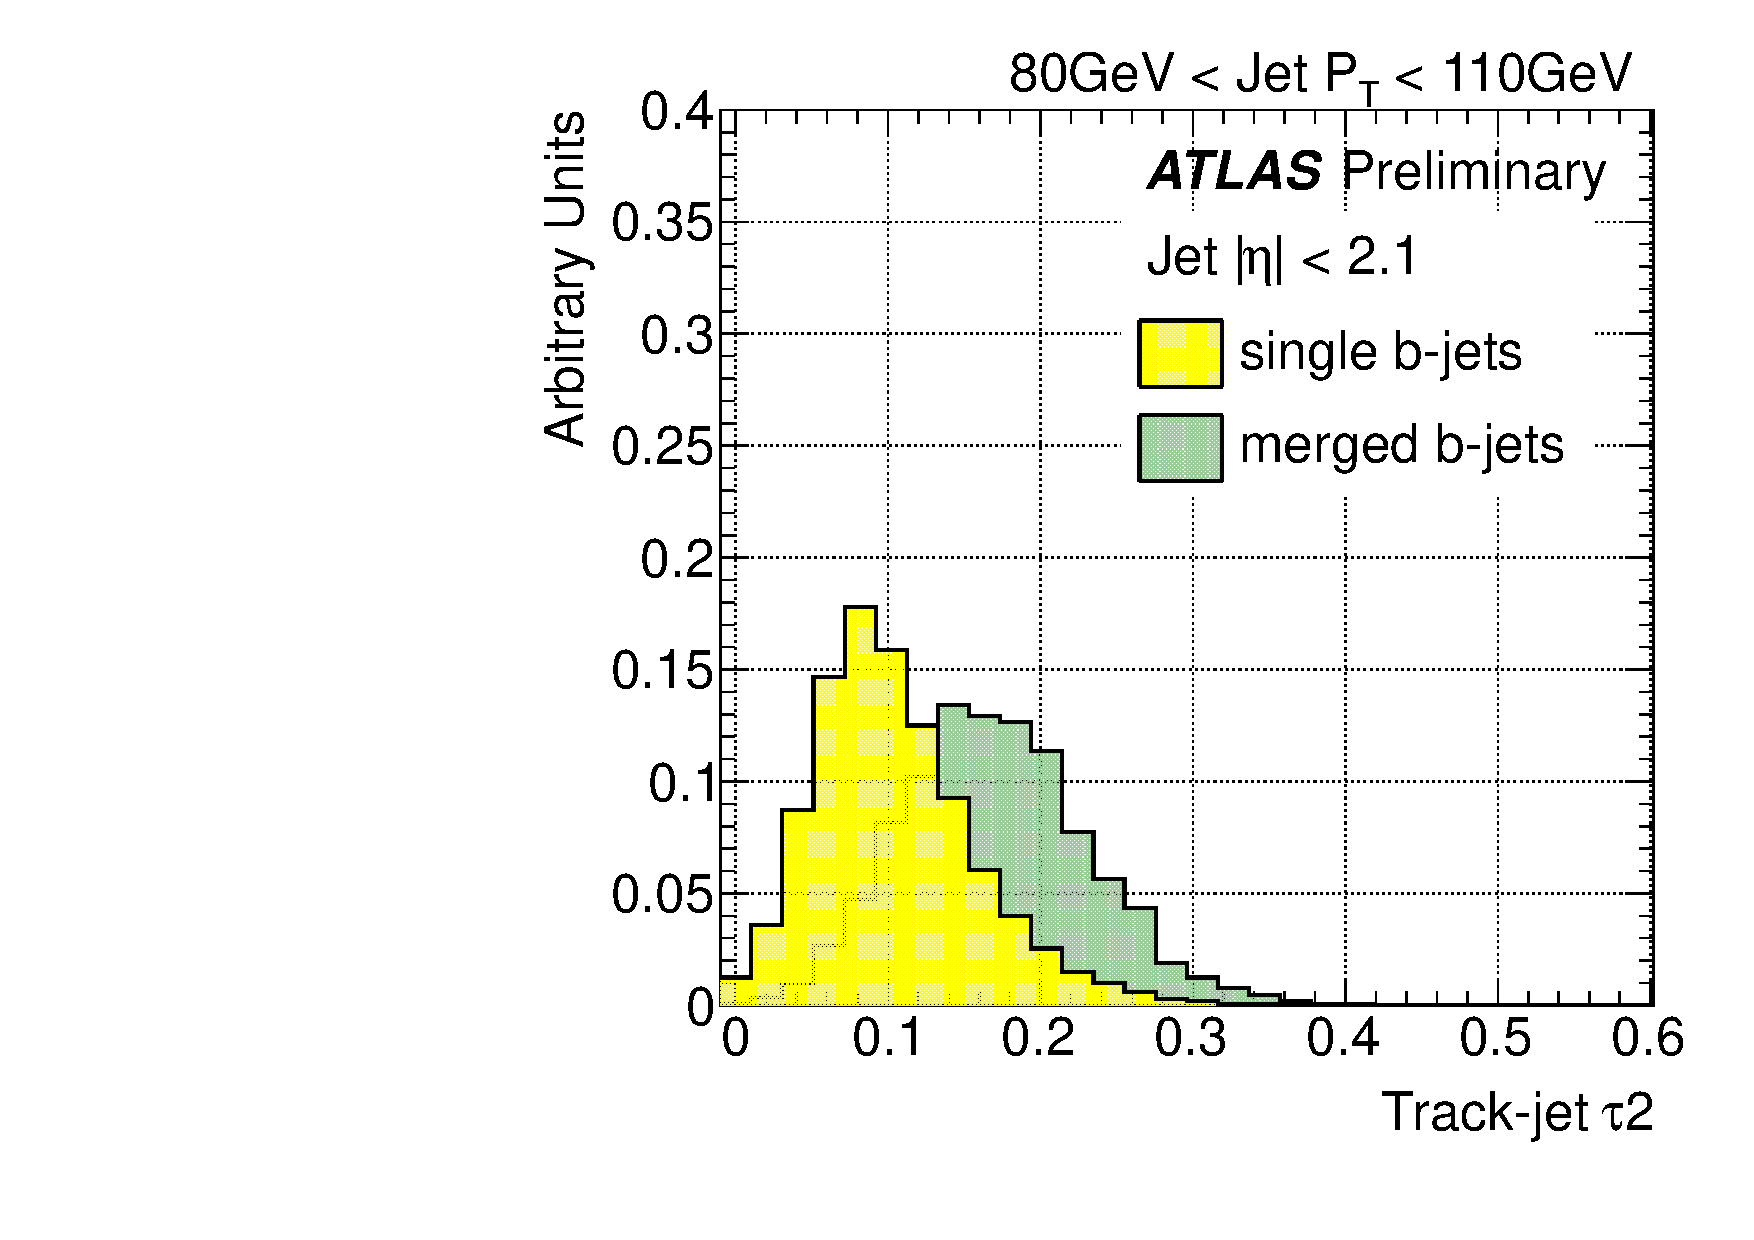
\includegraphics[width=0.49\textwidth]{FIGS/VarsSingleMerged/Tau2080.pdf}
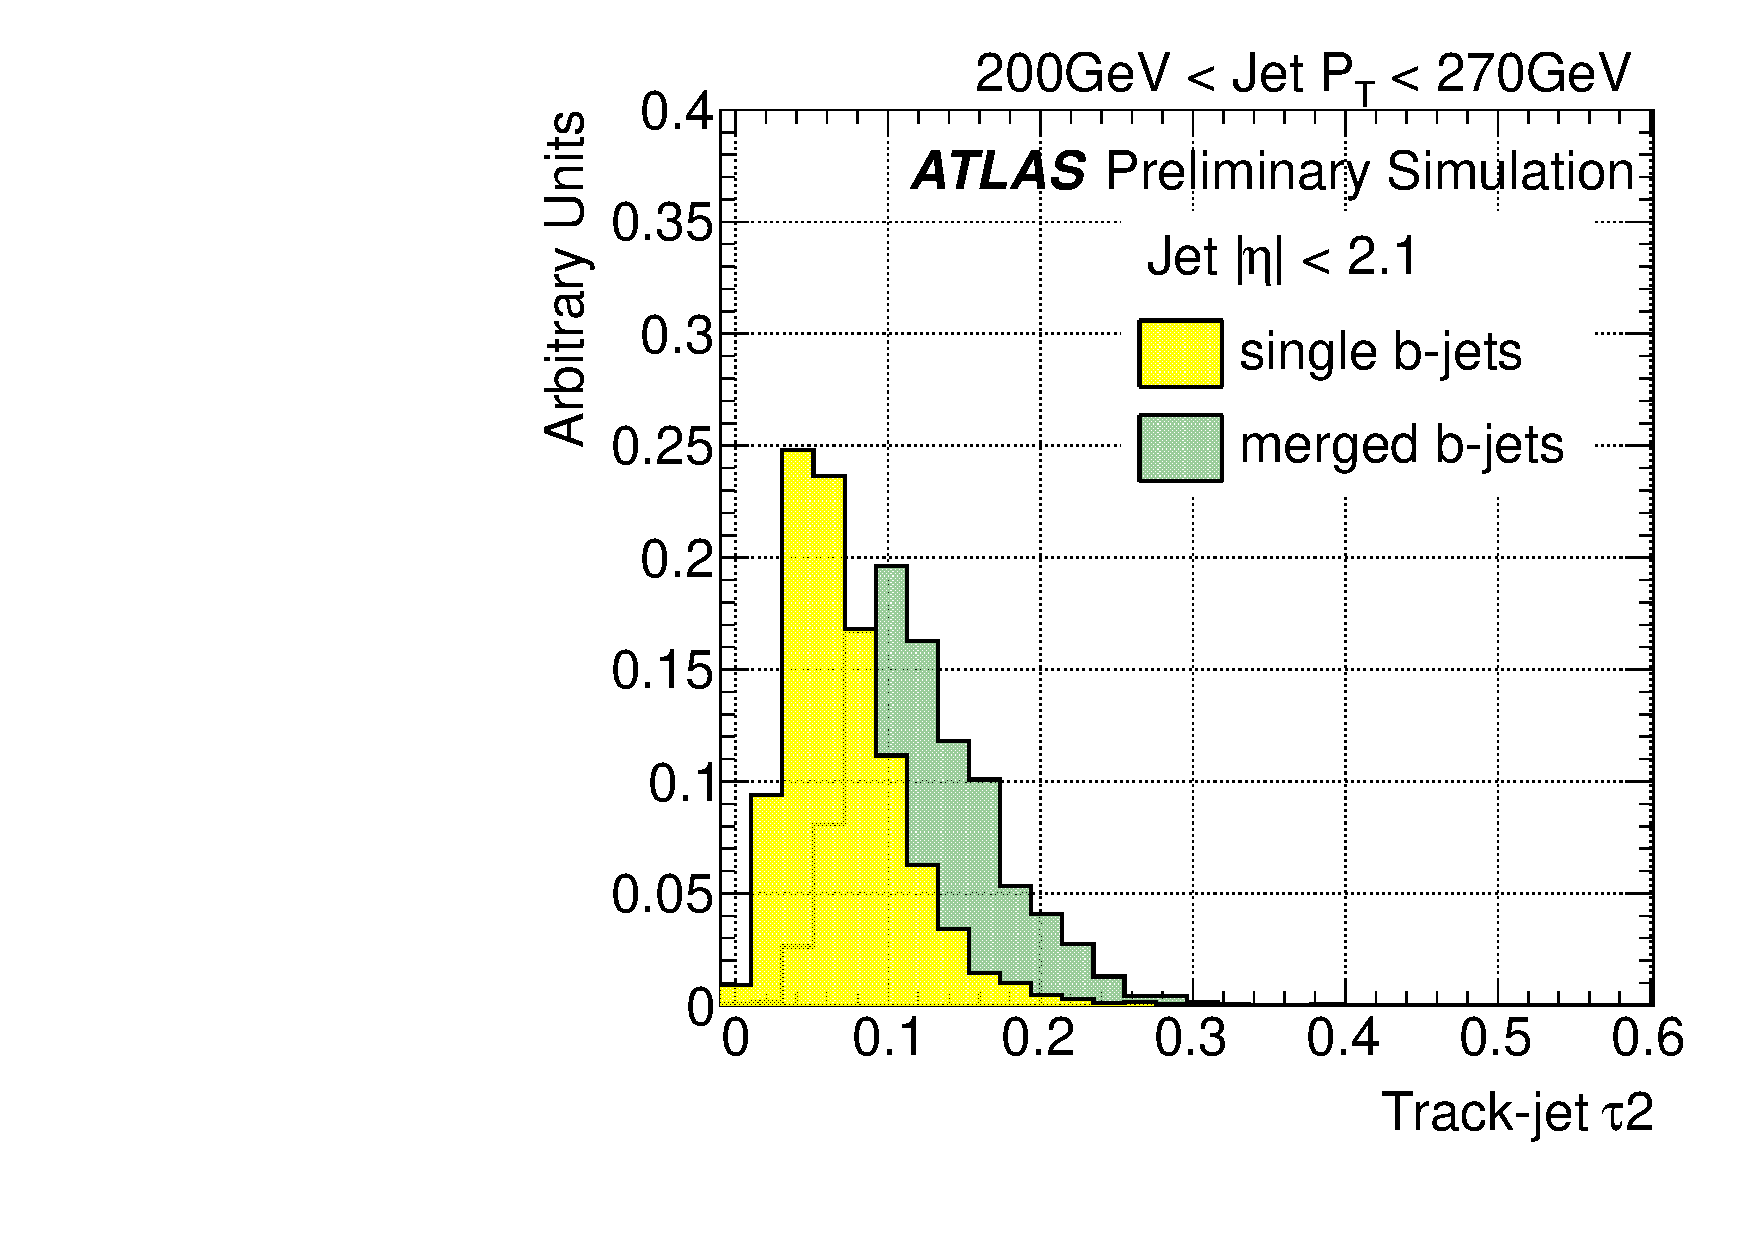
\includegraphics[width=0.49\textwidth]{FIGS/VarsSingleMerged/Tau2200.pdf}
\caption{Distribution of $\tau_2$ in jets for single and merged $b$-jets between 80~GeV to 110~GeV (left) and 200~GeV to 270~GeV (right).}
\label{fig:tau2singlemerged}
\end{figure}


\begin{figure}[tp]
\centering
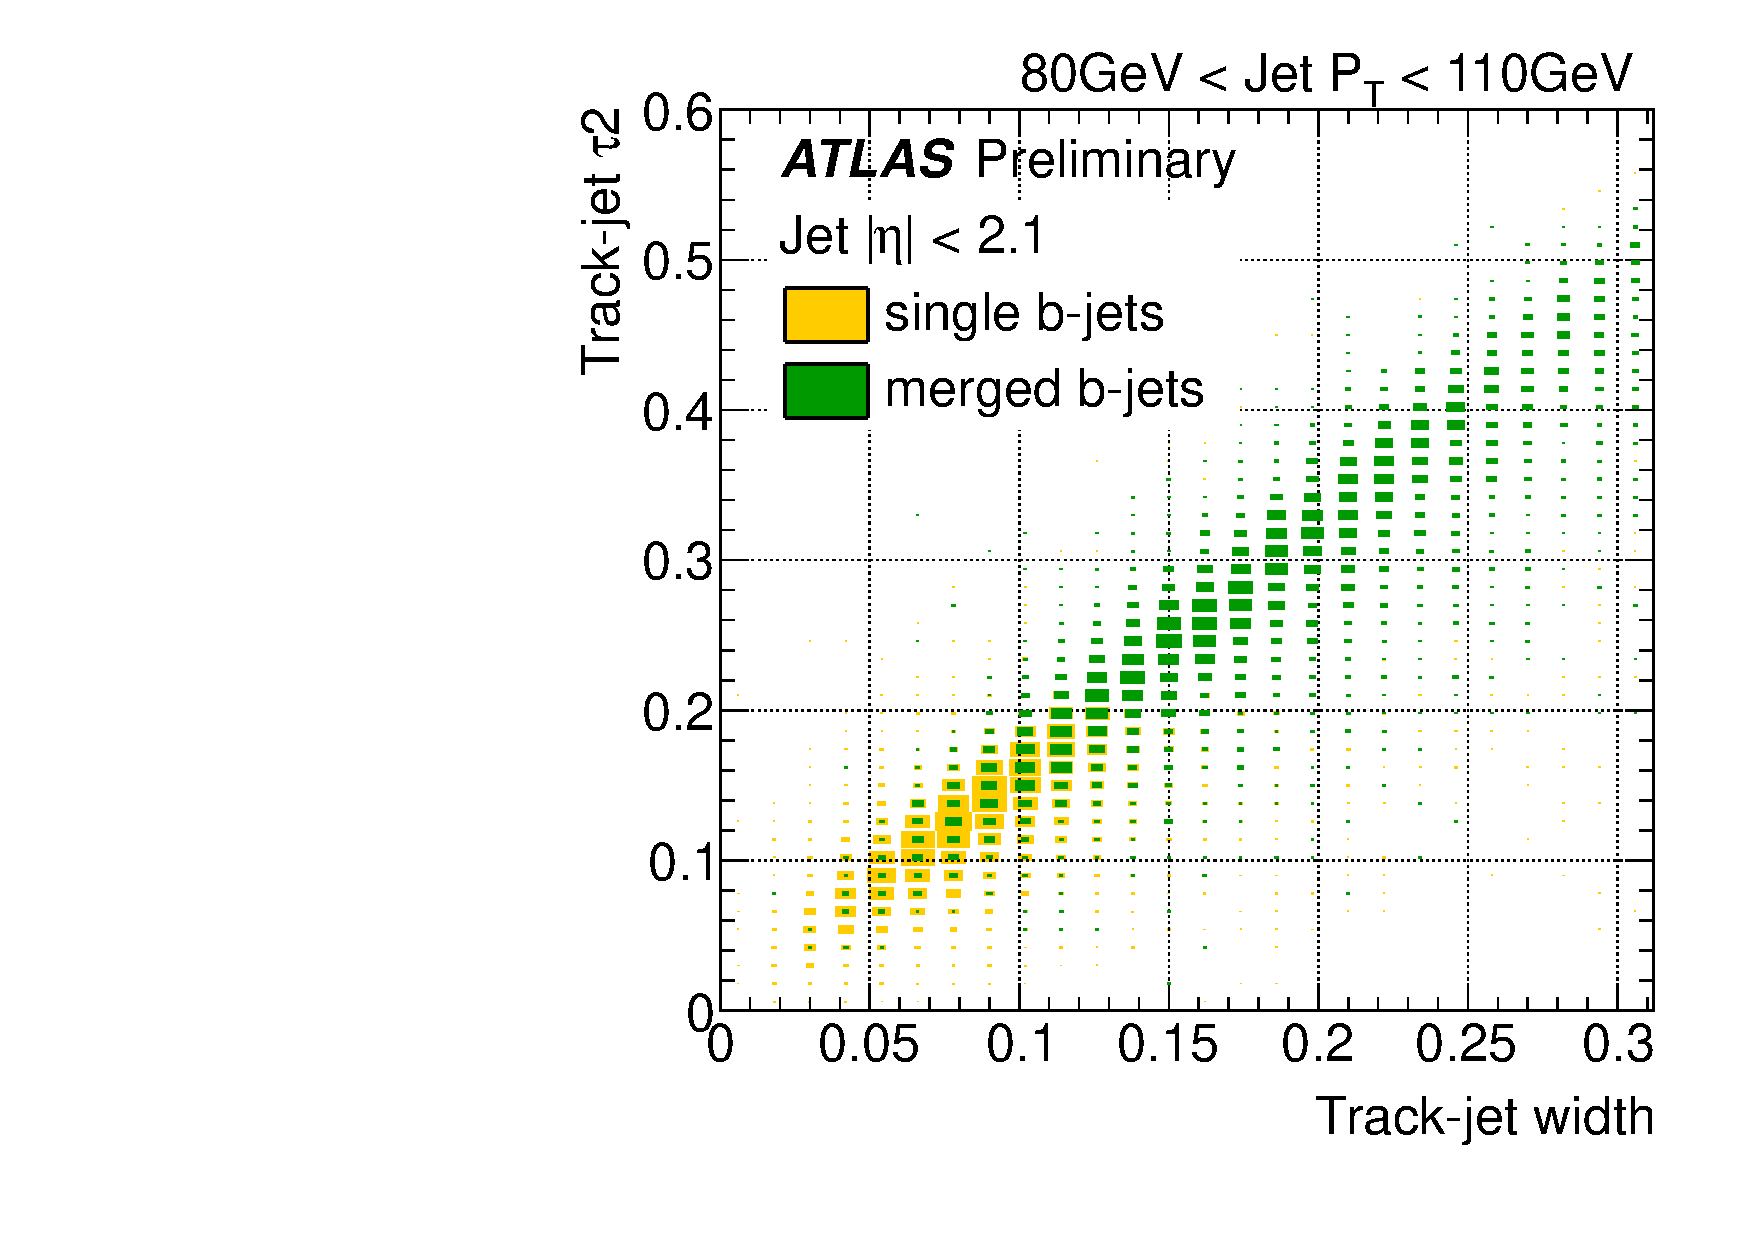
\includegraphics[width=0.49\textwidth]{FIGS/VarsSingleMerged/Tau2trkWidth080.pdf}
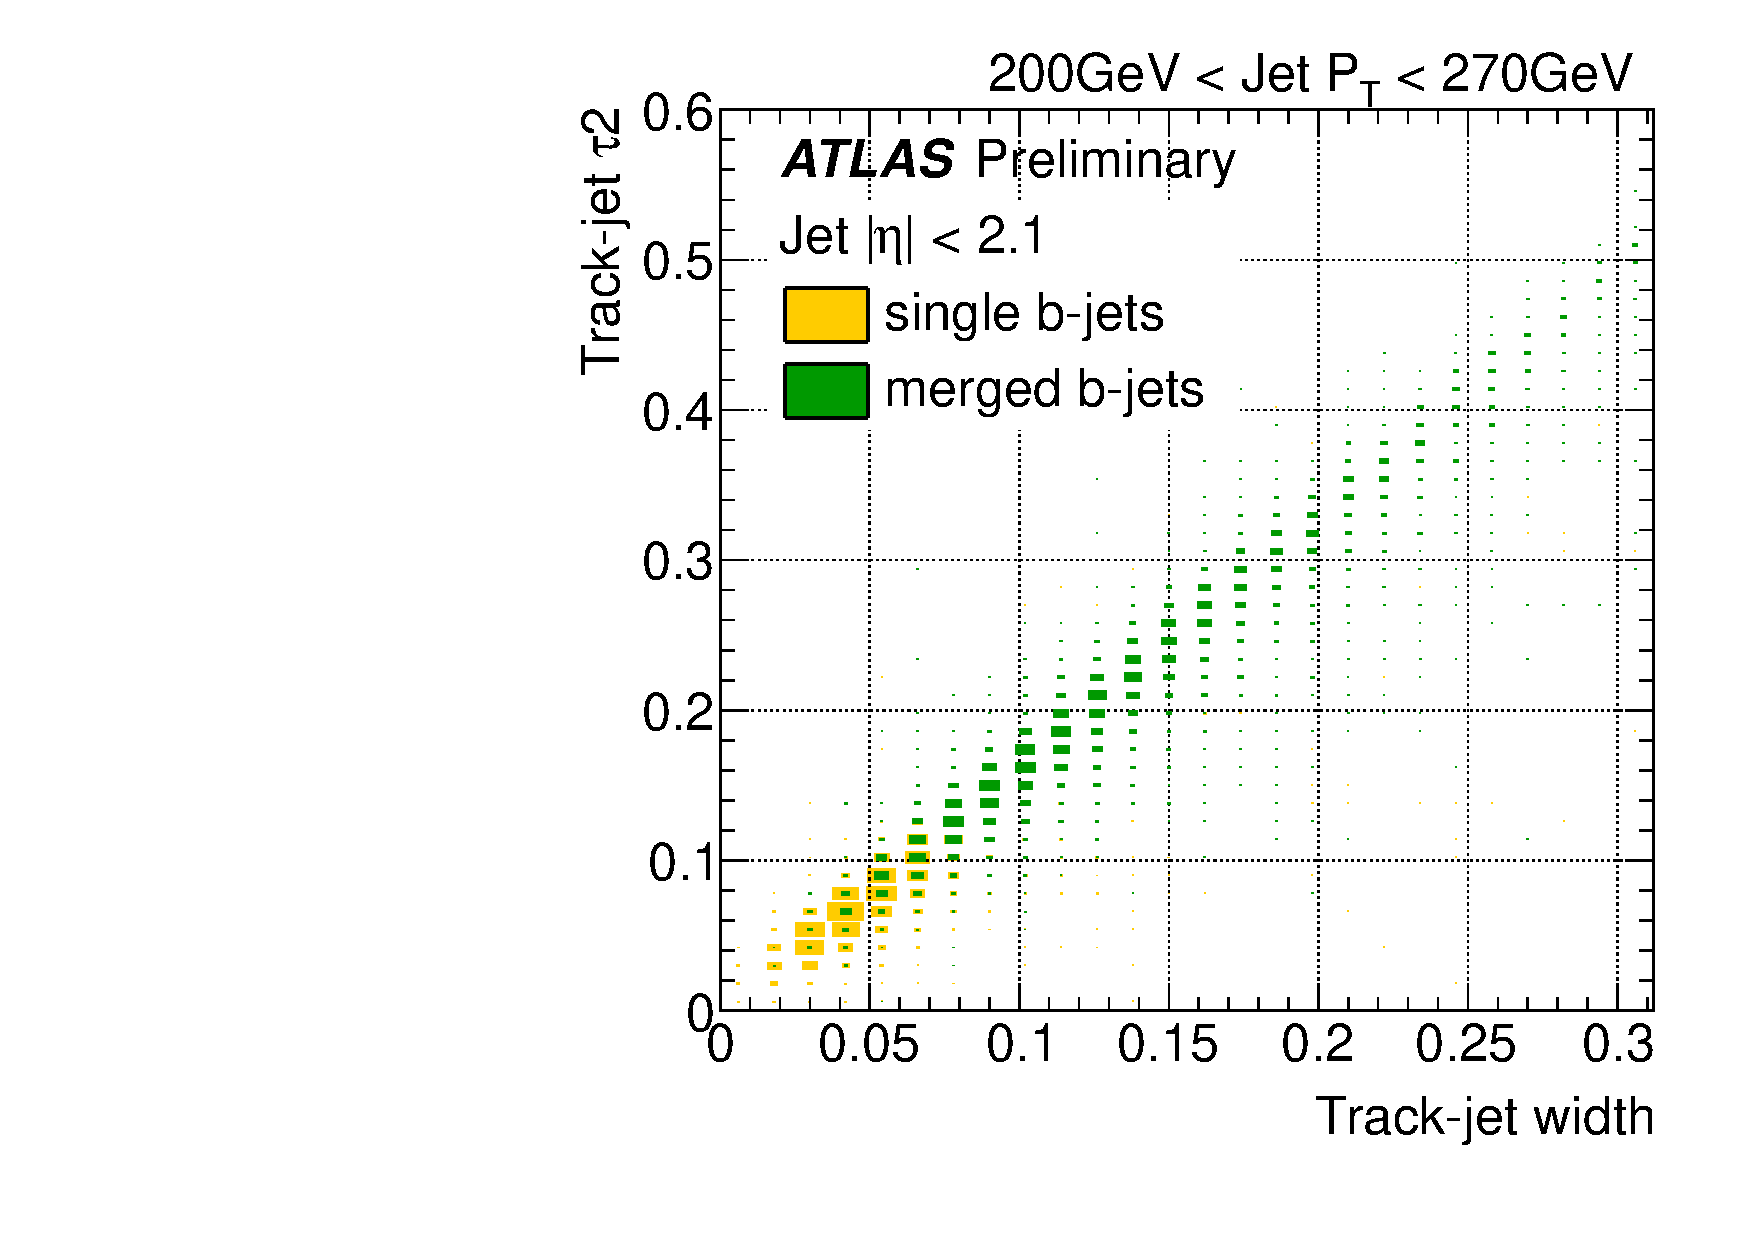
\includegraphics[width=0.49\textwidth]{FIGS/VarsSingleMerged/Tau2trkWidth200.pdf}
\caption{Correlation between $\tau _2$ and track-jet width for single and merged $b$-jets between 80~GeV to 110~GeV (left) and 200~GeV to 270~GeV (right).}
\label{fig:tau2trkwidthsinglemerged}
\end{figure}

\begin{figure}[tp]
\centering
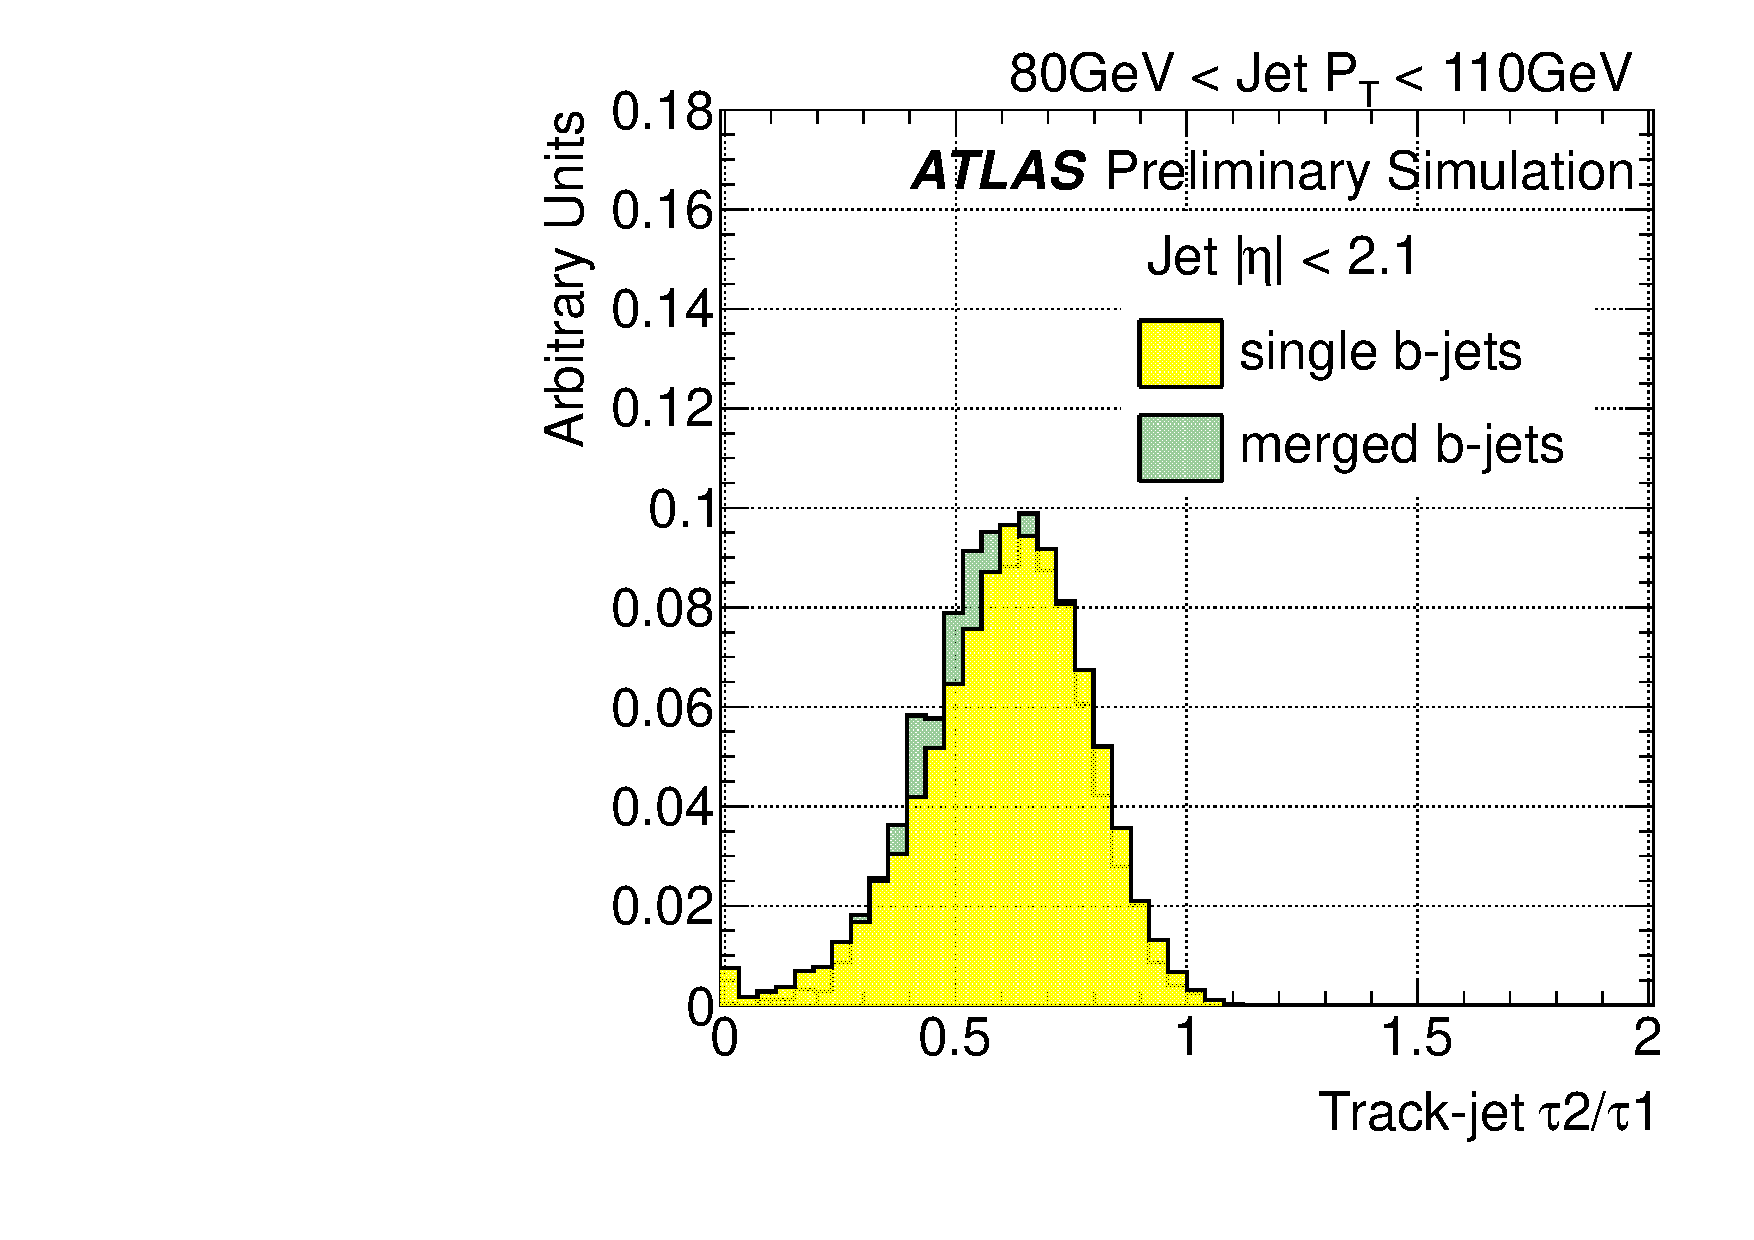
\includegraphics[width=0.49\textwidth]{FIGS/VarsSingleMerged/TauRatio080.pdf}
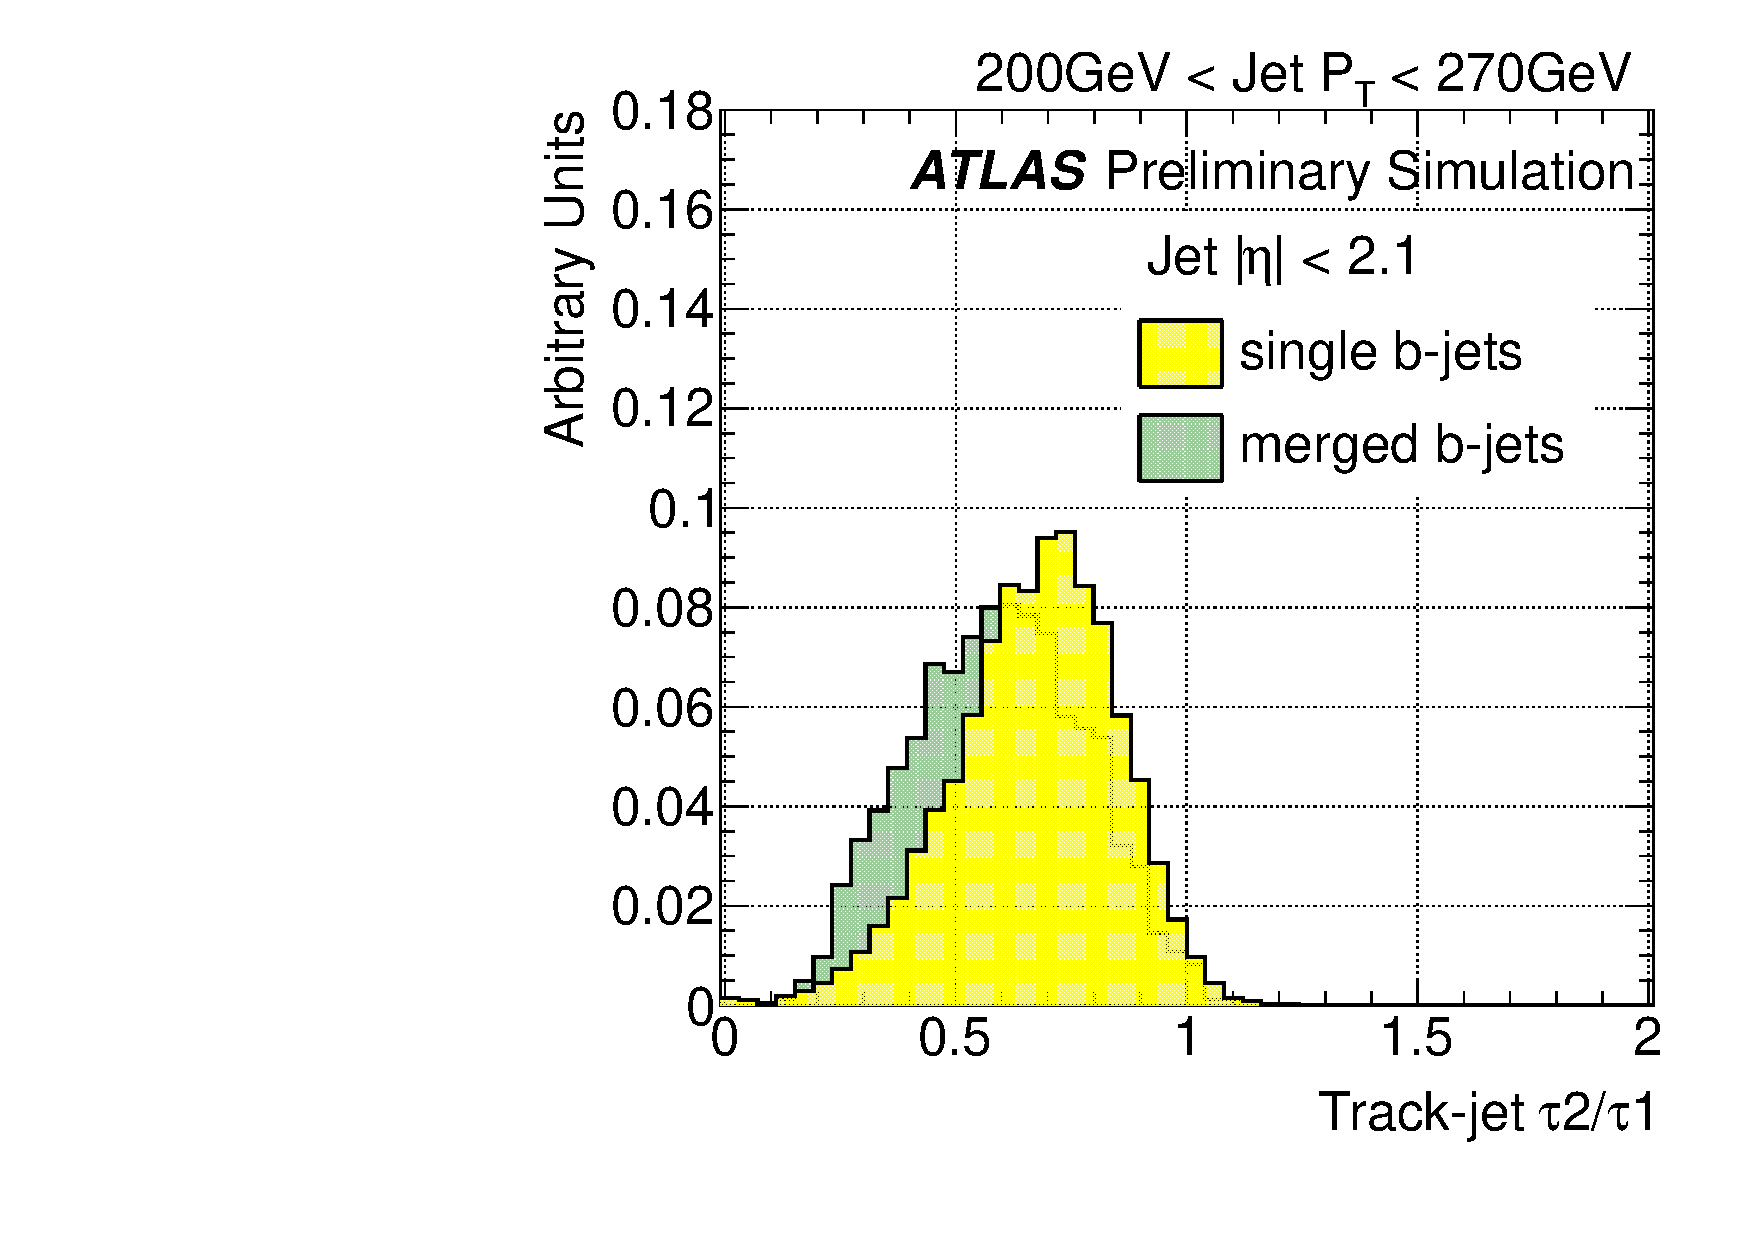
\includegraphics[width=0.49\textwidth]{FIGS/VarsSingleMerged/TauRatio200.pdf}
\caption{Distribution of $\tau_2/\tau_1$ in jets for single and merged $b$-jets between 80~GeV to 110~GeV (left) and 200~GeV to 270~GeV (right).}
\label{fig:tauratiosinglemerged}
\end{figure}


%Variables such as the $\DeltaR$ between the two leading constituents of the jet (those with highest transverse momentum) and the jet eccentricity (the ratio of the principal axes of the jet area) did not show good discrimination either and were not considered for the multivariate study.

{ \em VI. Jet Mass}
\\[3mm]

Figure~\ref{fig:masssinglemerged} shows the distribution of the jet mass for single and merged $b$-jets.
\\[3mm]

\begin{figure}[tp]
\centering
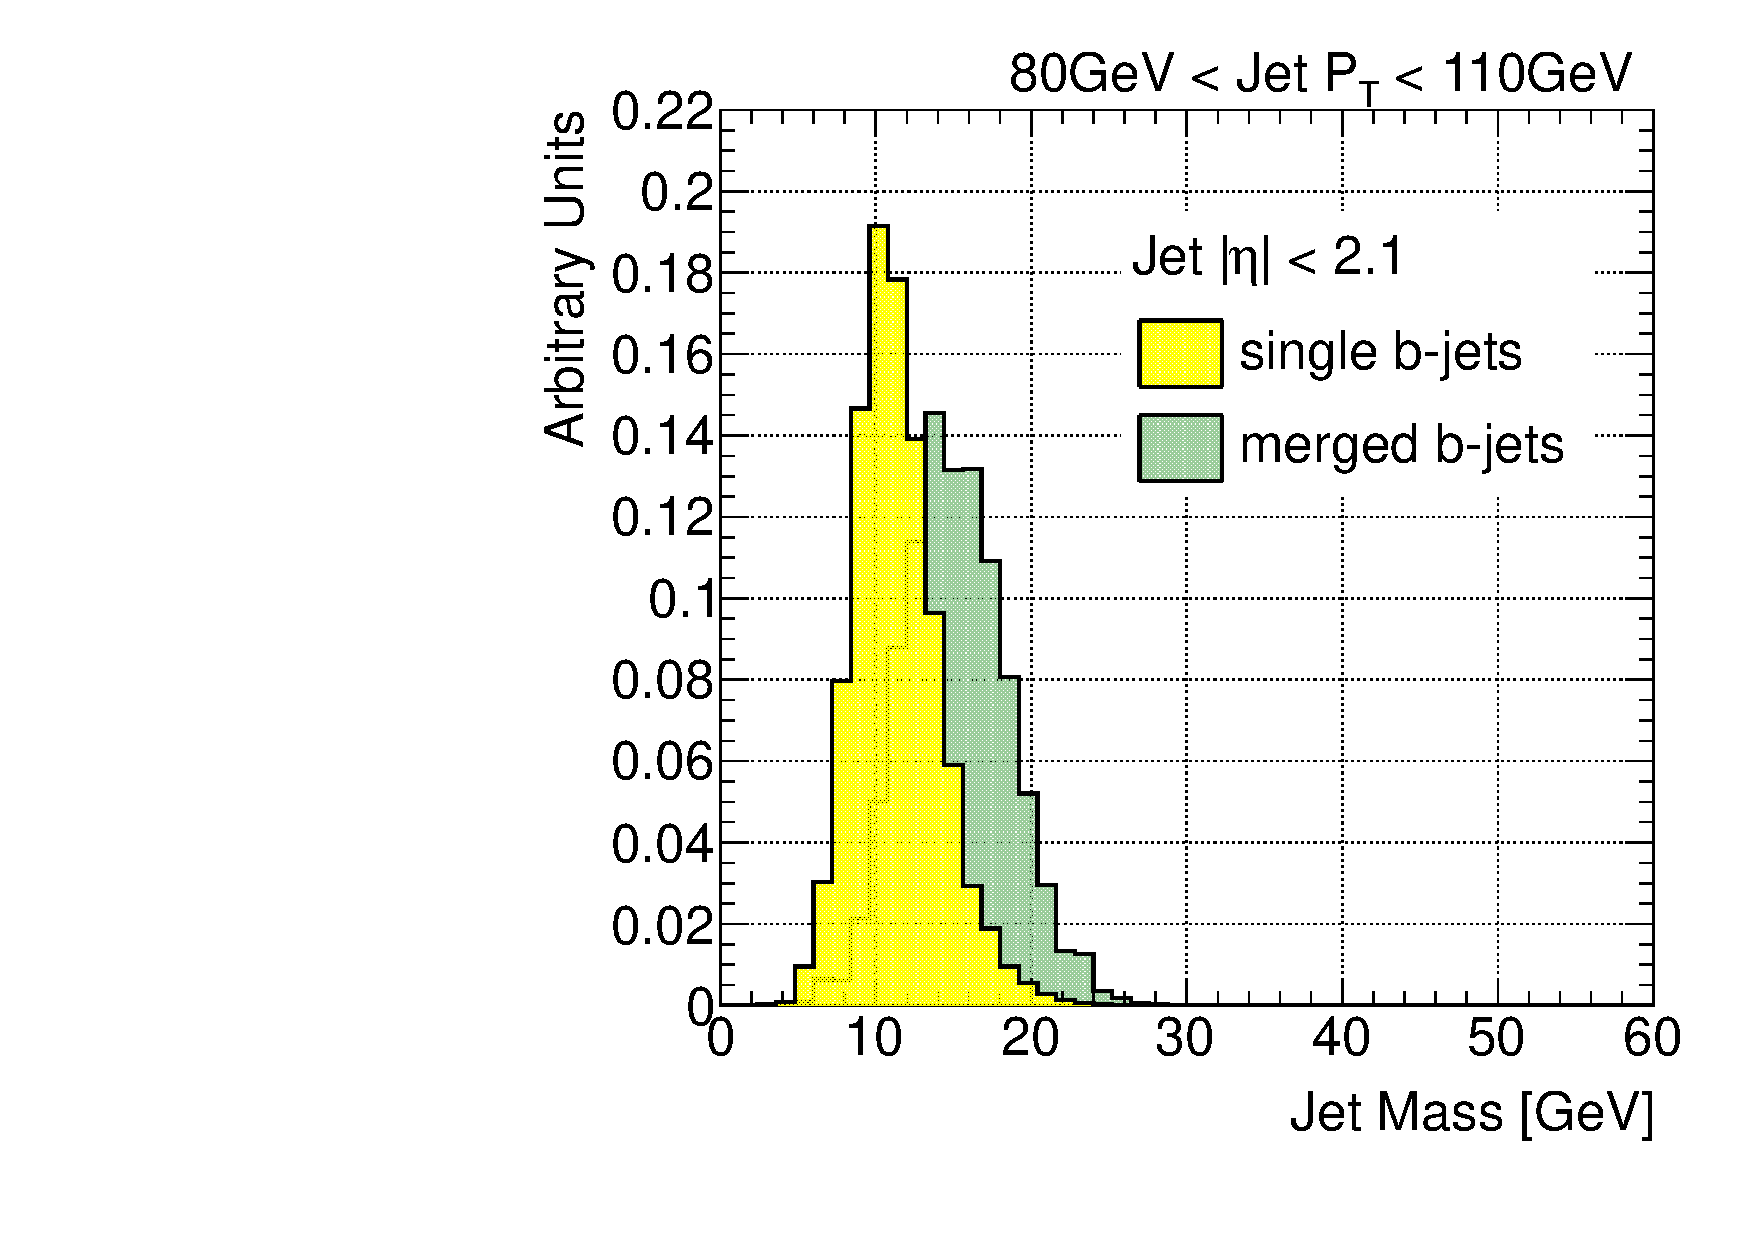
\includegraphics[width=0.49\textwidth]{FIGS/VarsSingleMerged/JetMass080.pdf}
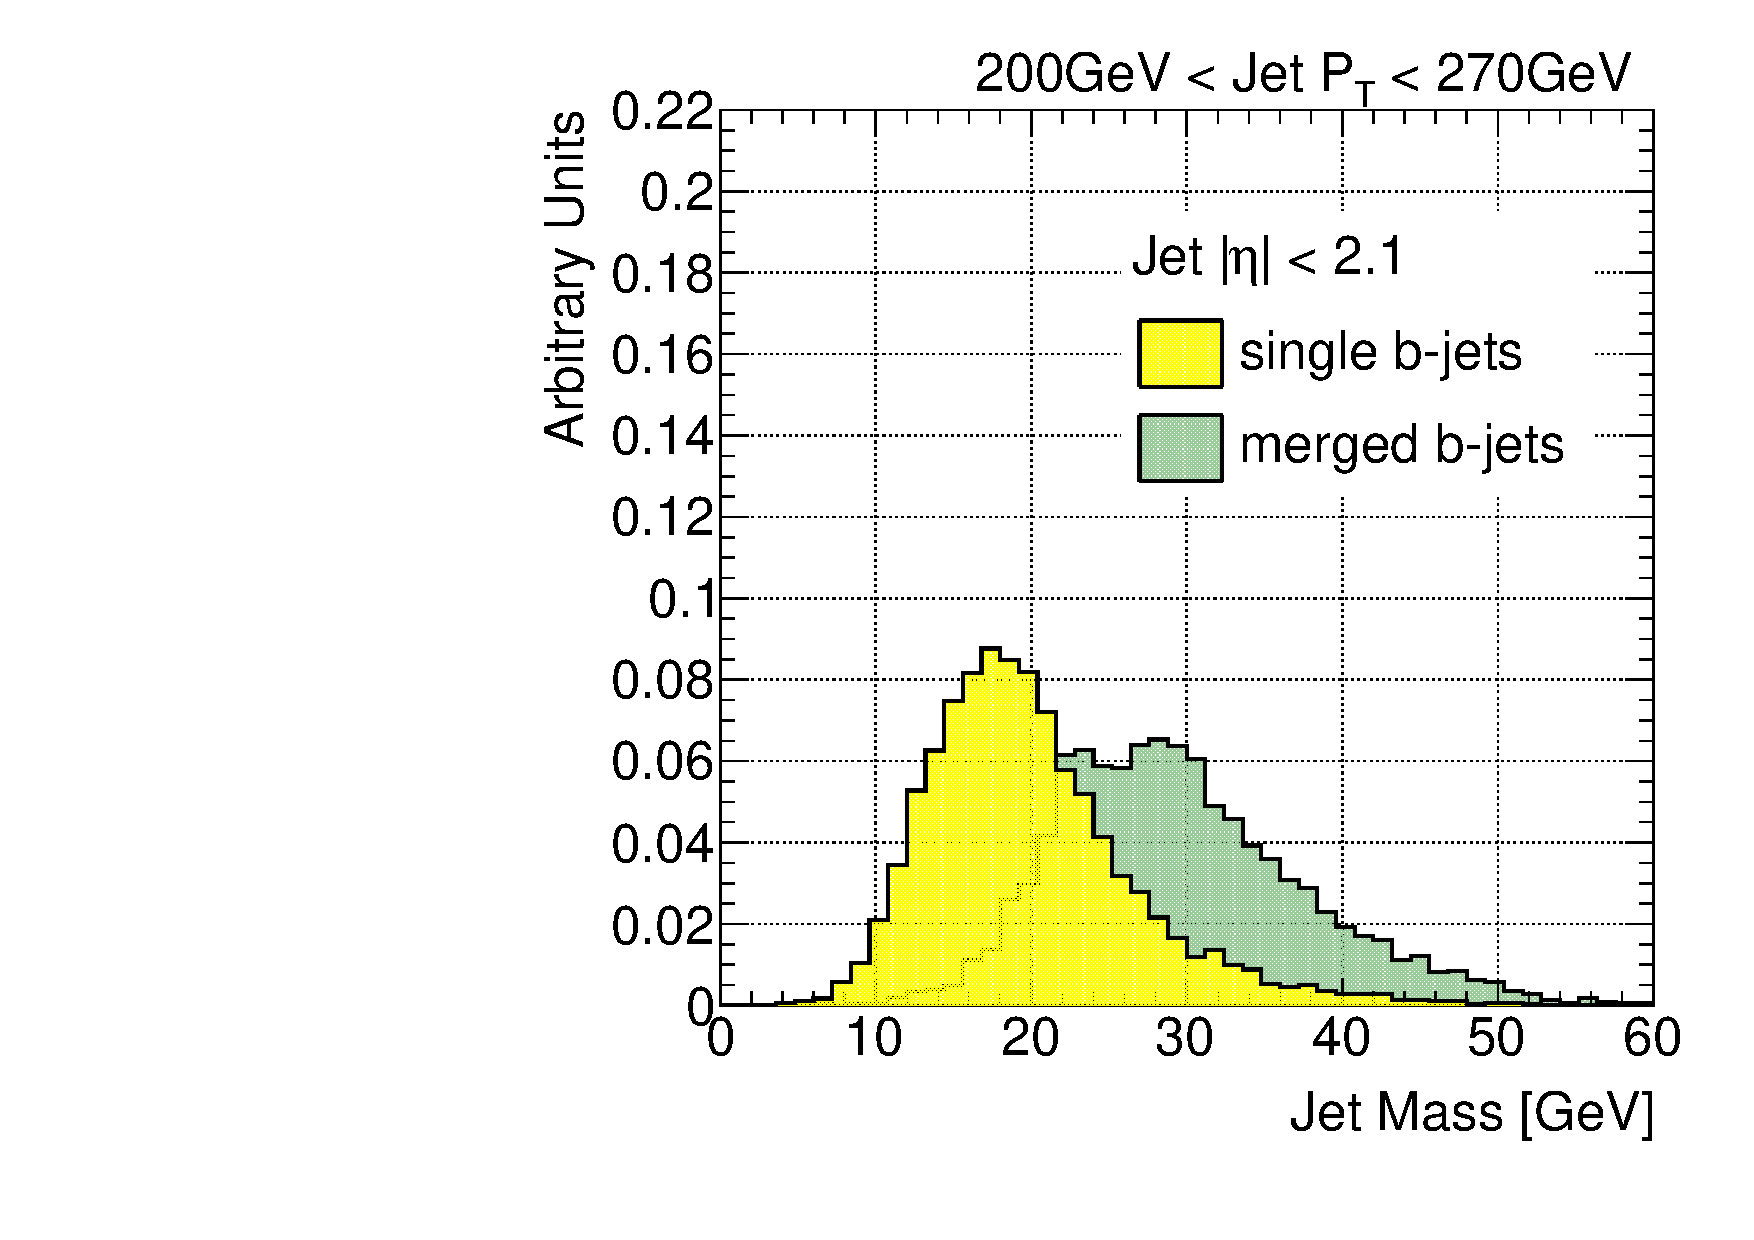
\includegraphics[width=0.49\textwidth]{FIGS/VarsSingleMerged/JetMass200.pdf}
\caption{Distribution of jet mass in~GeV for single and merged $b$-jets between 80~GeV to 110~GeV (left) and 200~GeV to 270~GeV (right).}
\label{fig:masssinglemerged}
\end{figure}

{ \em VII. Number of $k_t$ subjets}
\\[3mm]

Figure~\ref{fig:nsubjetsinglemerged} shows the distribution of the number of sub-track-jets single and merged $b$-jets.
\\[3mm]

\begin{figure}[tp]
\centering
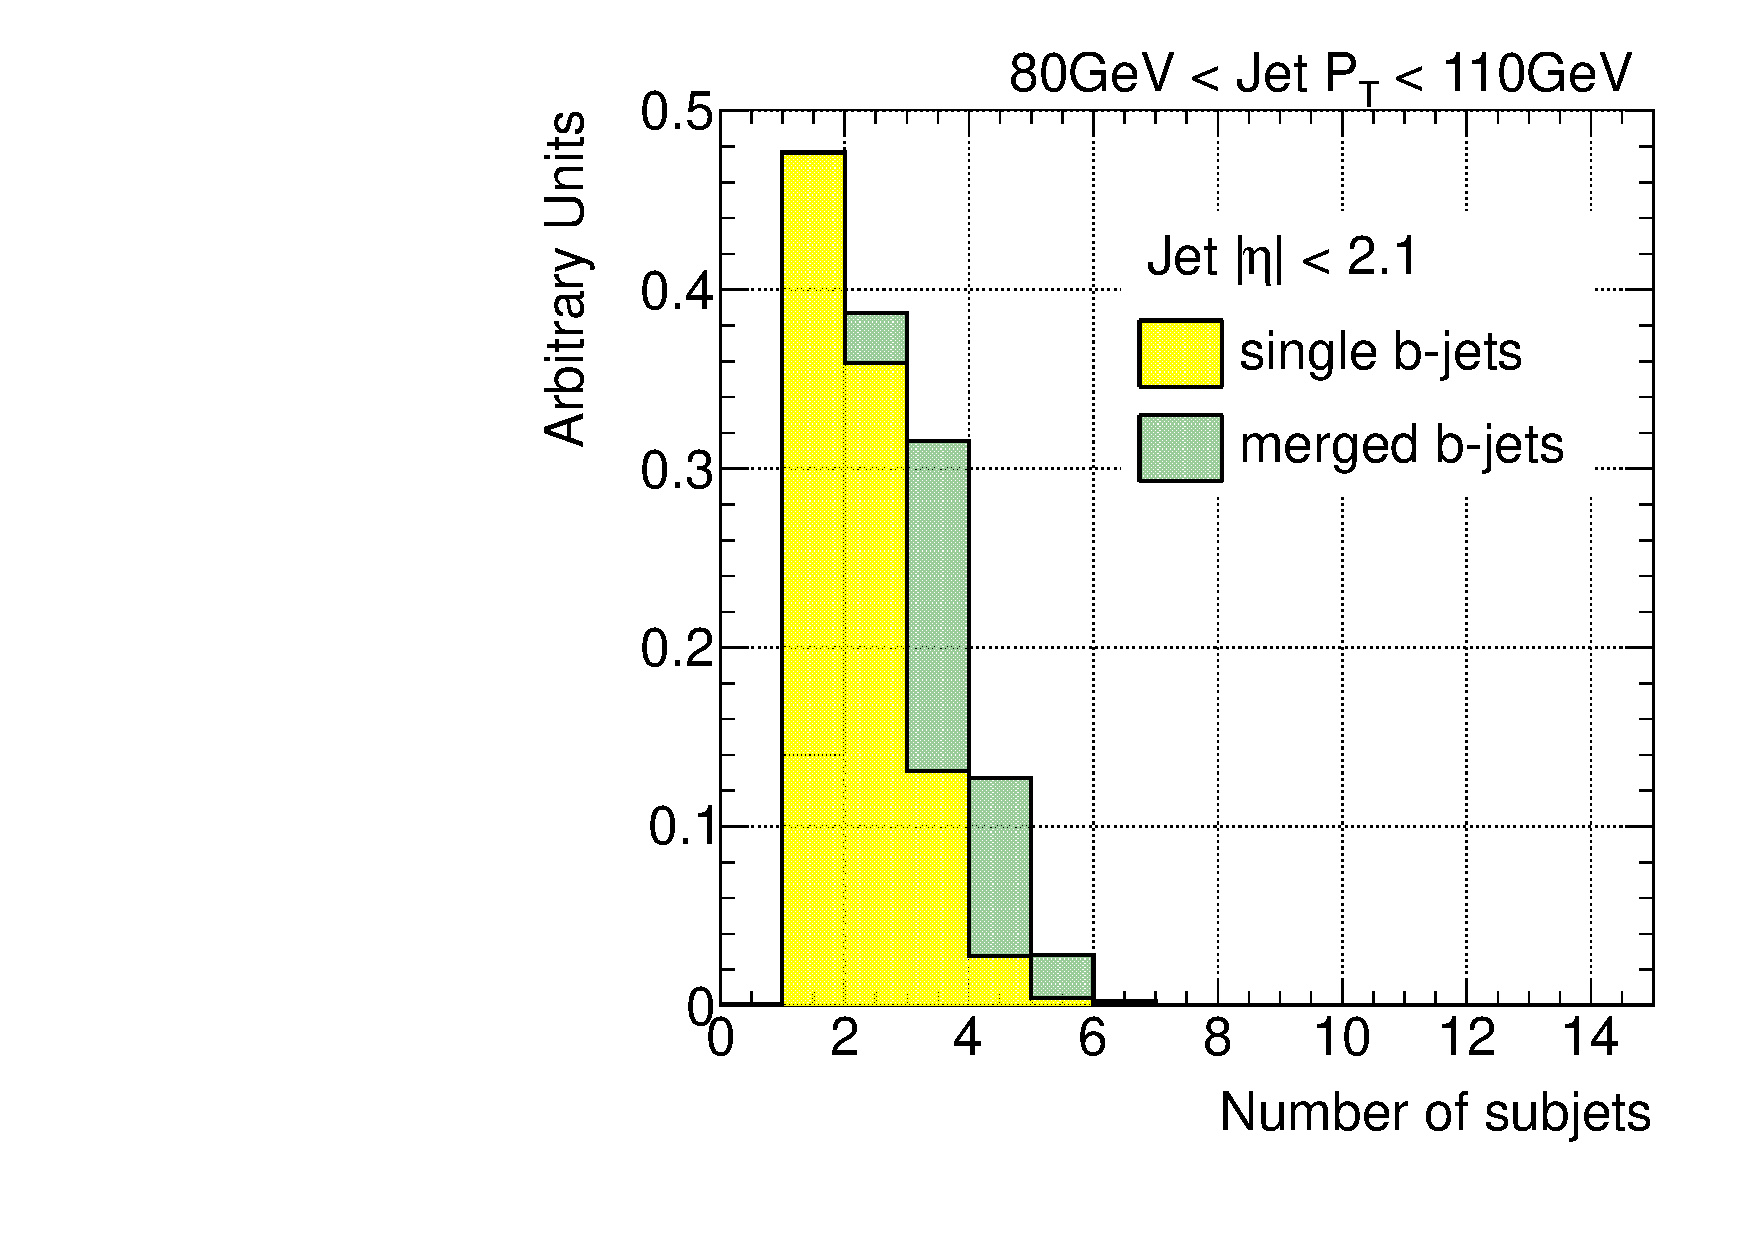
\includegraphics[width=0.49\textwidth]{FIGS/VarsSingleMerged/Nsubjets080.pdf}
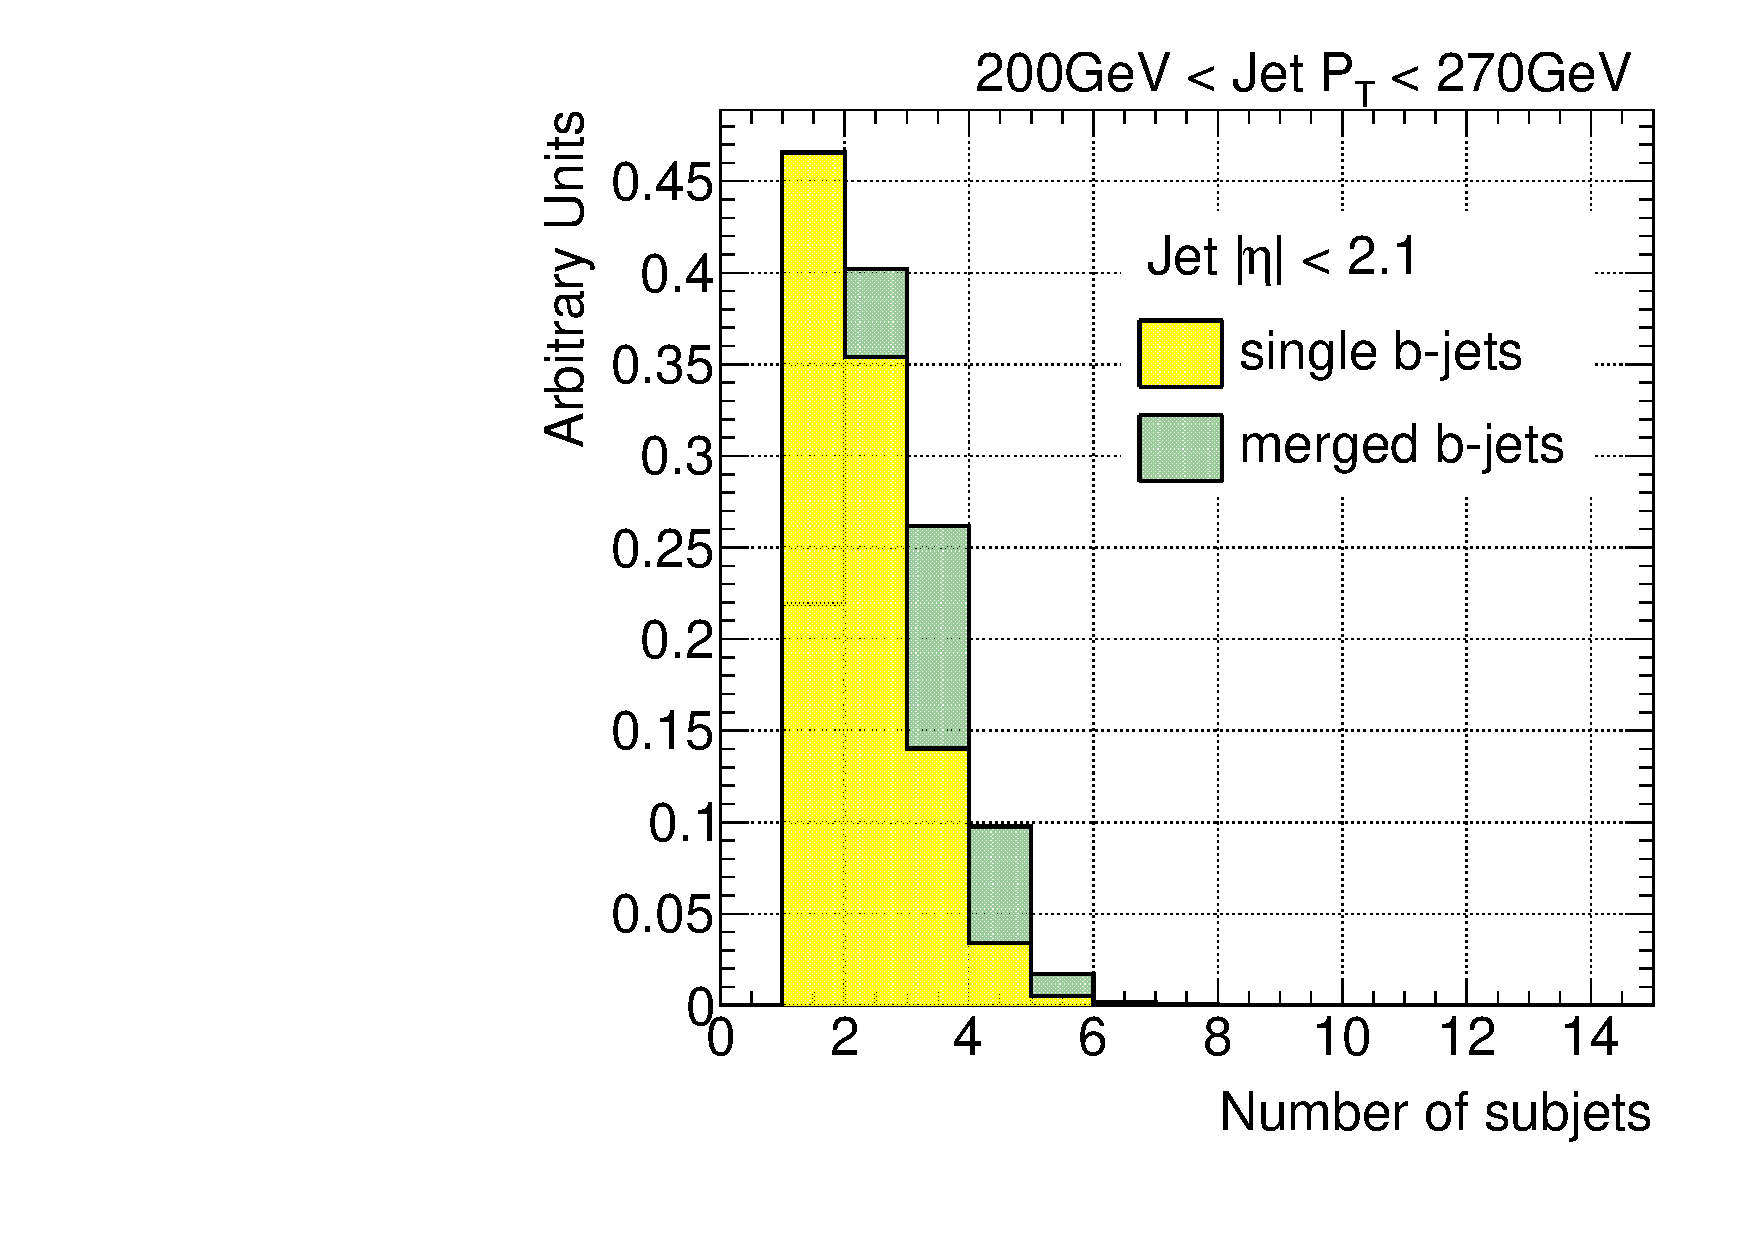
\includegraphics[width=0.49\textwidth]{FIGS/VarsSingleMerged/Nsubjets200.pdf}
\caption{Distribution of the number of $k_t$ sub-track-jets for single and merged $b$-jets between 80~GeV to 110~GeV (left) and 200~GeV to 270~GeV (right).}
\label{fig:nsubjetsinglemerged}
\end{figure}


{ \em VIII. $\Delta R$ between leading constituents}
\\[3mm]

Figure~\ref{fig:drtrk12singlemerged} shows the distribution of the number  $\Delta R$ between leading tracks in the jet for single and merged $b$-jets.
\\[3mm]

\begin{figure}[tp]
\centering
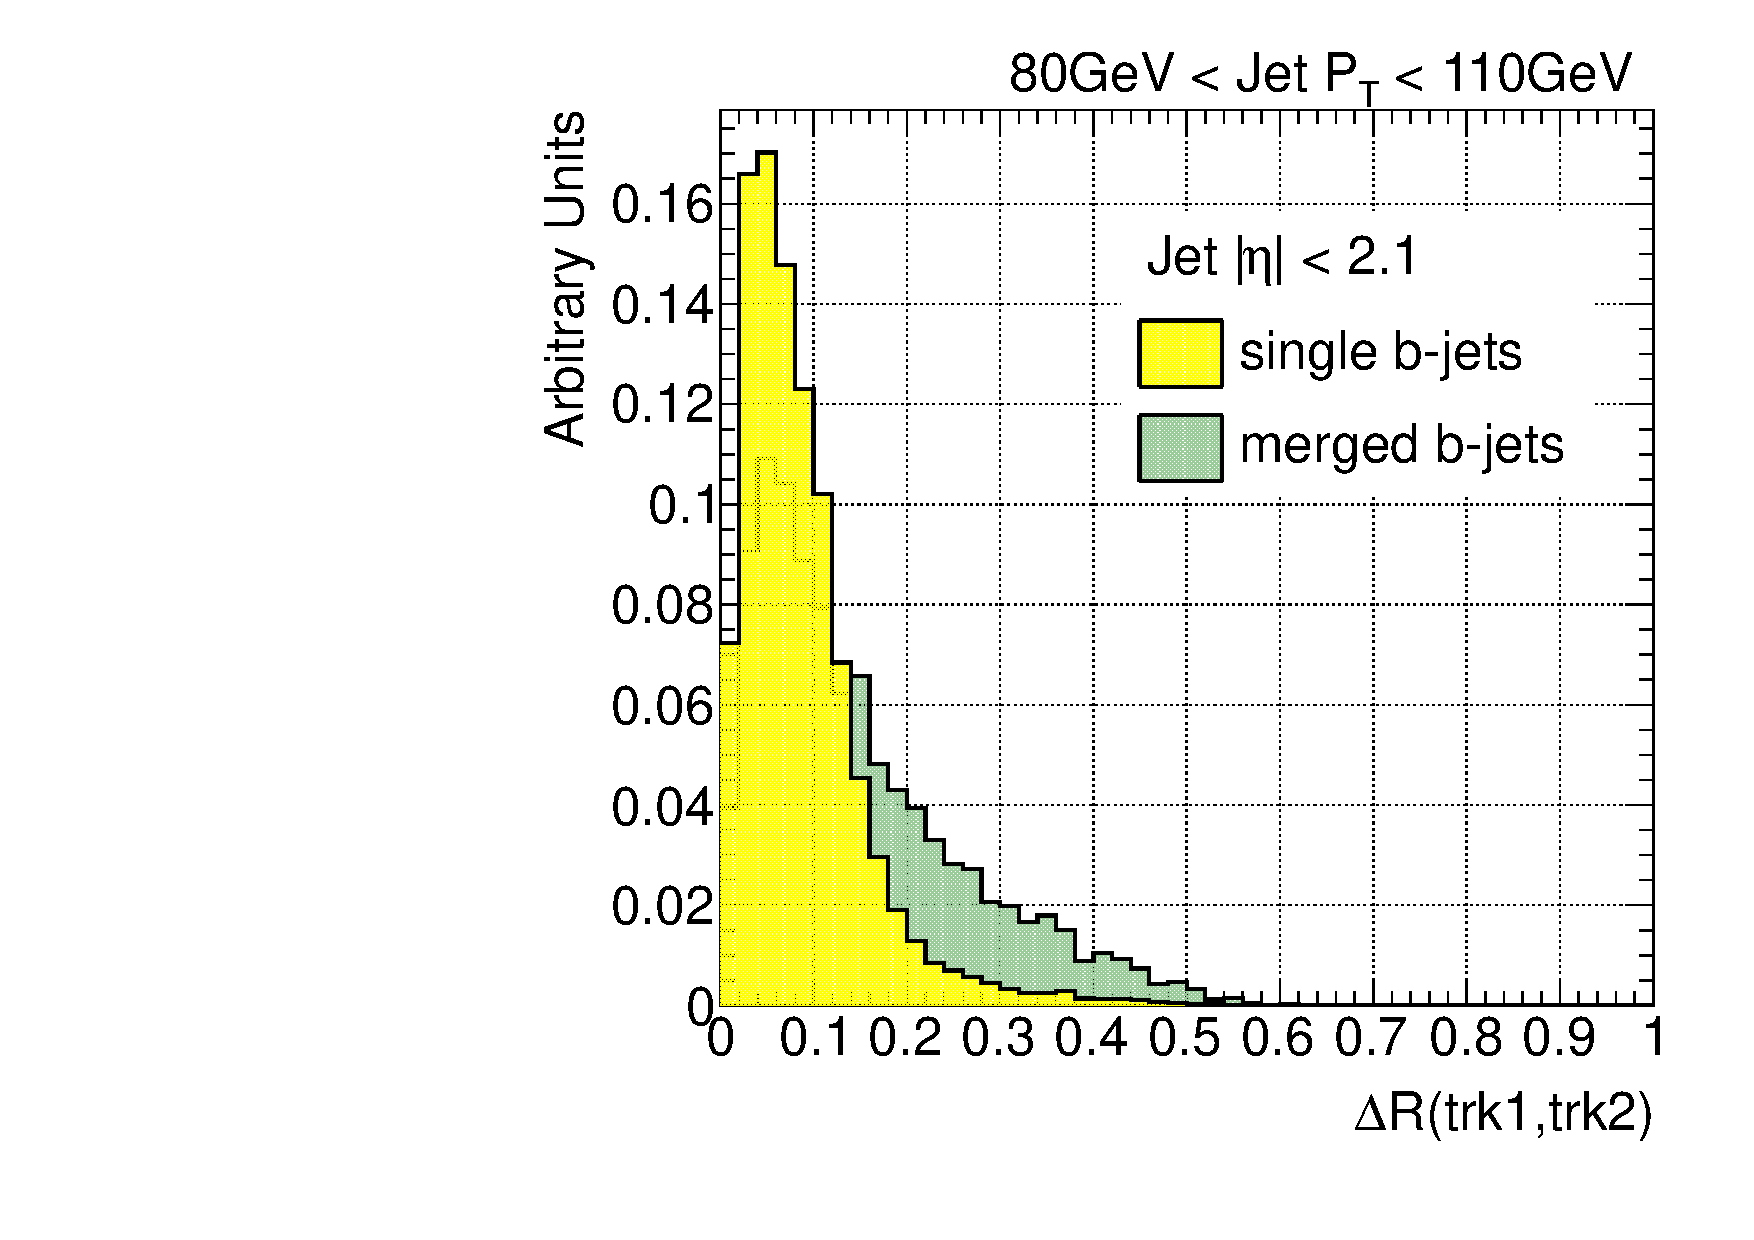
\includegraphics[width=0.49\textwidth]{FIGS/VarsSingleMerged/DRtrk12080.pdf}
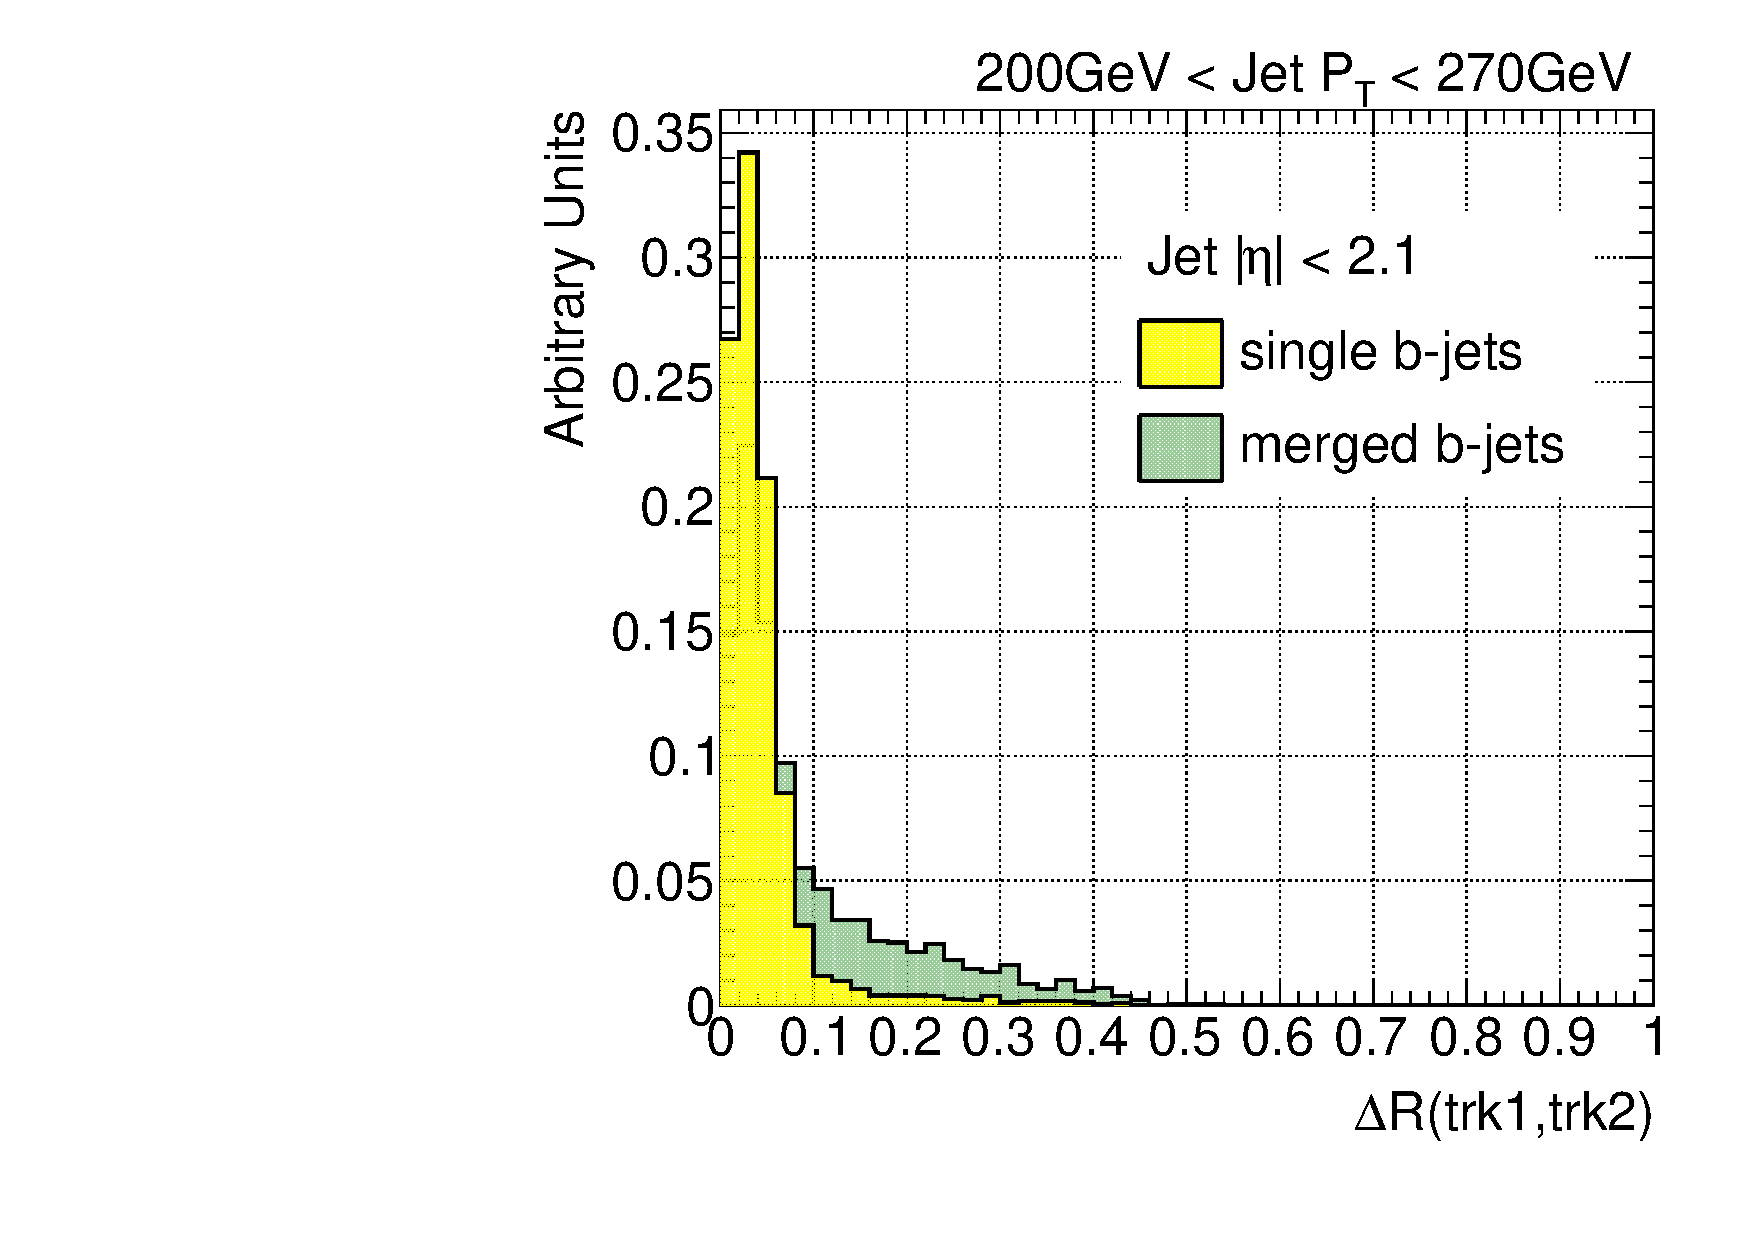
\includegraphics[width=0.49\textwidth]{FIGS/VarsSingleMerged/DRtrk12200.pdf}
\caption{Distribution of $\Delta R$ between leading tracks for single and merged $b$-jets between 80~GeV to 110~GeV (left) and 200~GeV to 270~GeV (right).}
\label{fig:drtrk12singlemerged}
\end{figure}


{ \em IX. Jet eccentricity}
\\[3mm]

Figure~\ref{fig:jeteccsinglemerged} shows the distribution of the jet track-eccentricity for single and merged $b$-jets.
\\[3mm]

\begin{figure}[tp]
\centering
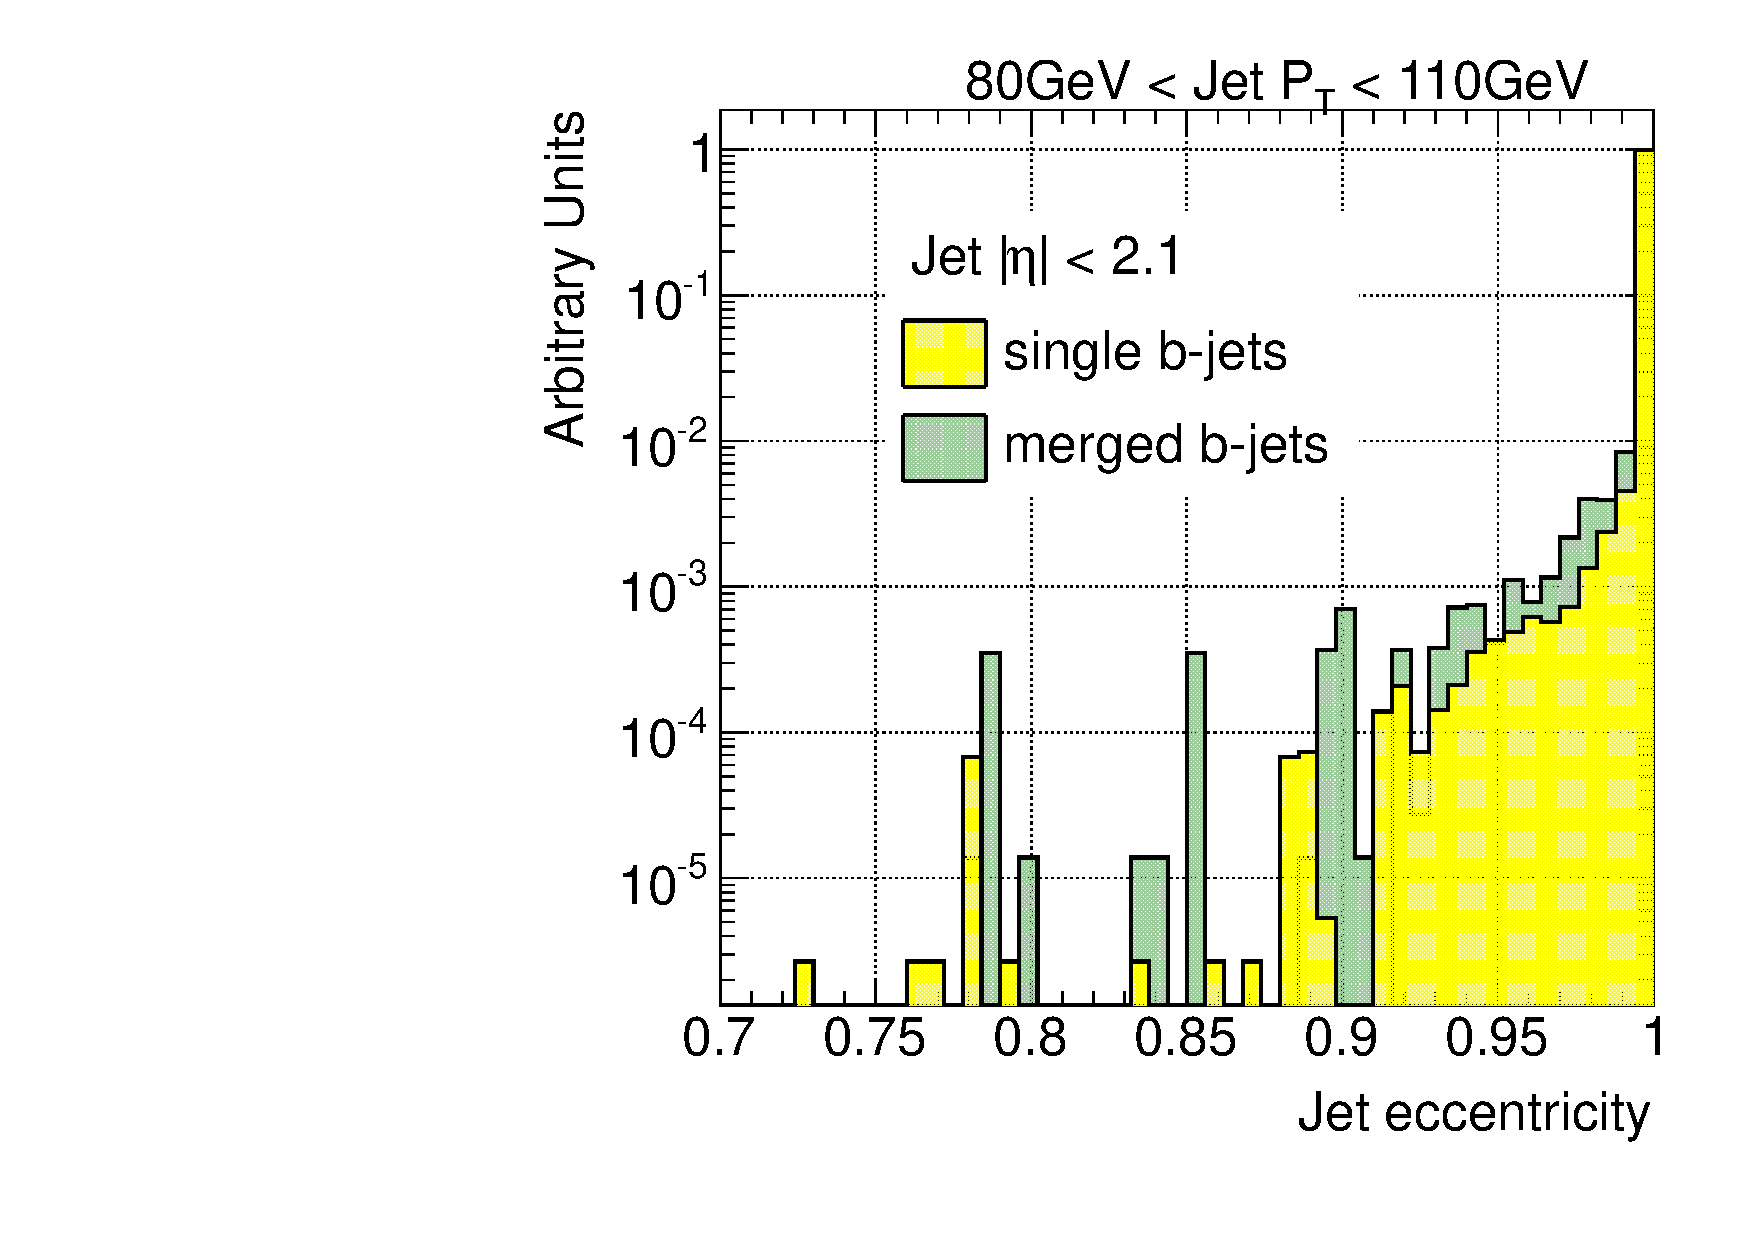
\includegraphics[width=0.49\textwidth]{FIGS/VarsSingleMerged/JetEcc080.pdf}
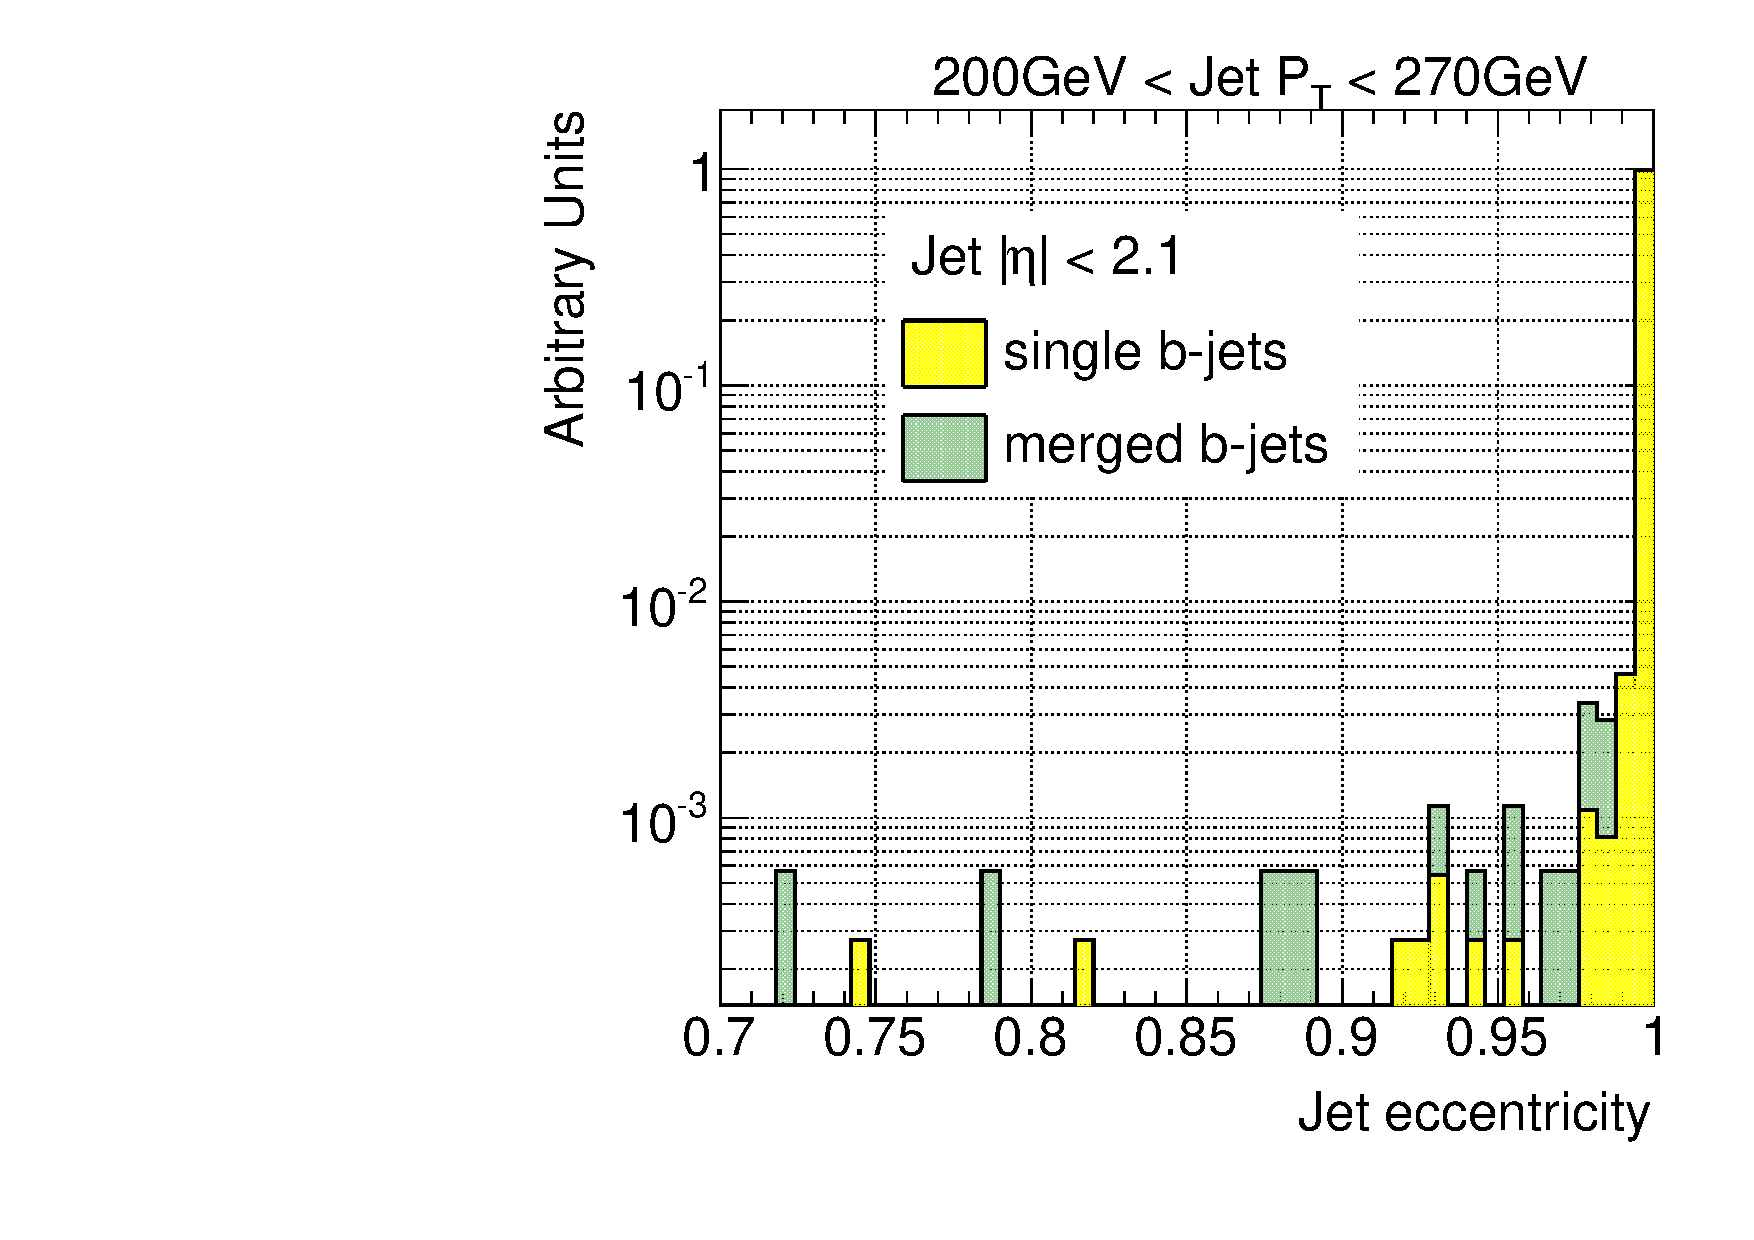
\includegraphics[width=0.49\textwidth]{FIGS/VarsSingleMerged/JetEcc200.pdf}
\caption{Distribution of the jet eccentricity for single and merged $b$-jets between 80~GeV to 110~GeV (left) and 200~GeV to 270~GeV (right).}
\label{fig:jeteccsinglemerged}
\end{figure}


We also explored the potential improvement of constructing kinematic variables with only displaced tracks, as these are the ones expected to arise from the decay of B-hadrons. Cuts of 2, 2.5 and 3 on the track transverse impact parameter significance were investigated leading however to no gain in discrimation power.

 In Figures~\ref{fig:displacedntrk} and~\ref{fig:displacedtrkwidth} two examples are shown.

\begin{figure}[tp]
\centering
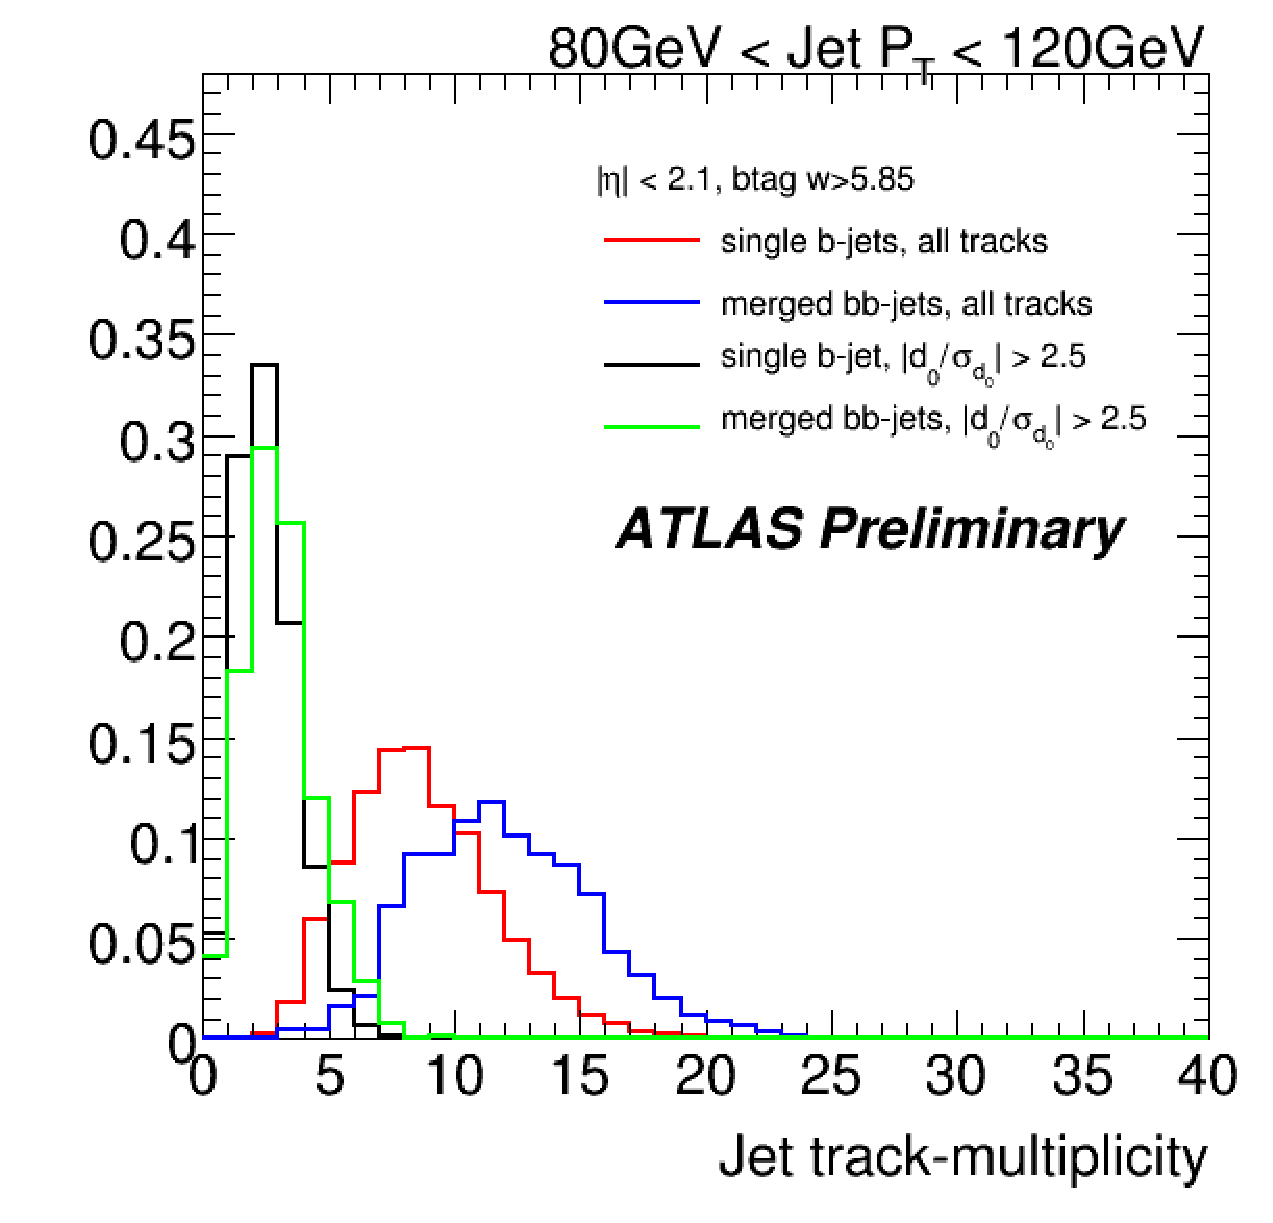
\includegraphics[width=0.49\textwidth]{FIGS/TEMPFigs/DisplacedTracks/ntrk_singlemerged_AllandDisplaced_80-120.pdf}
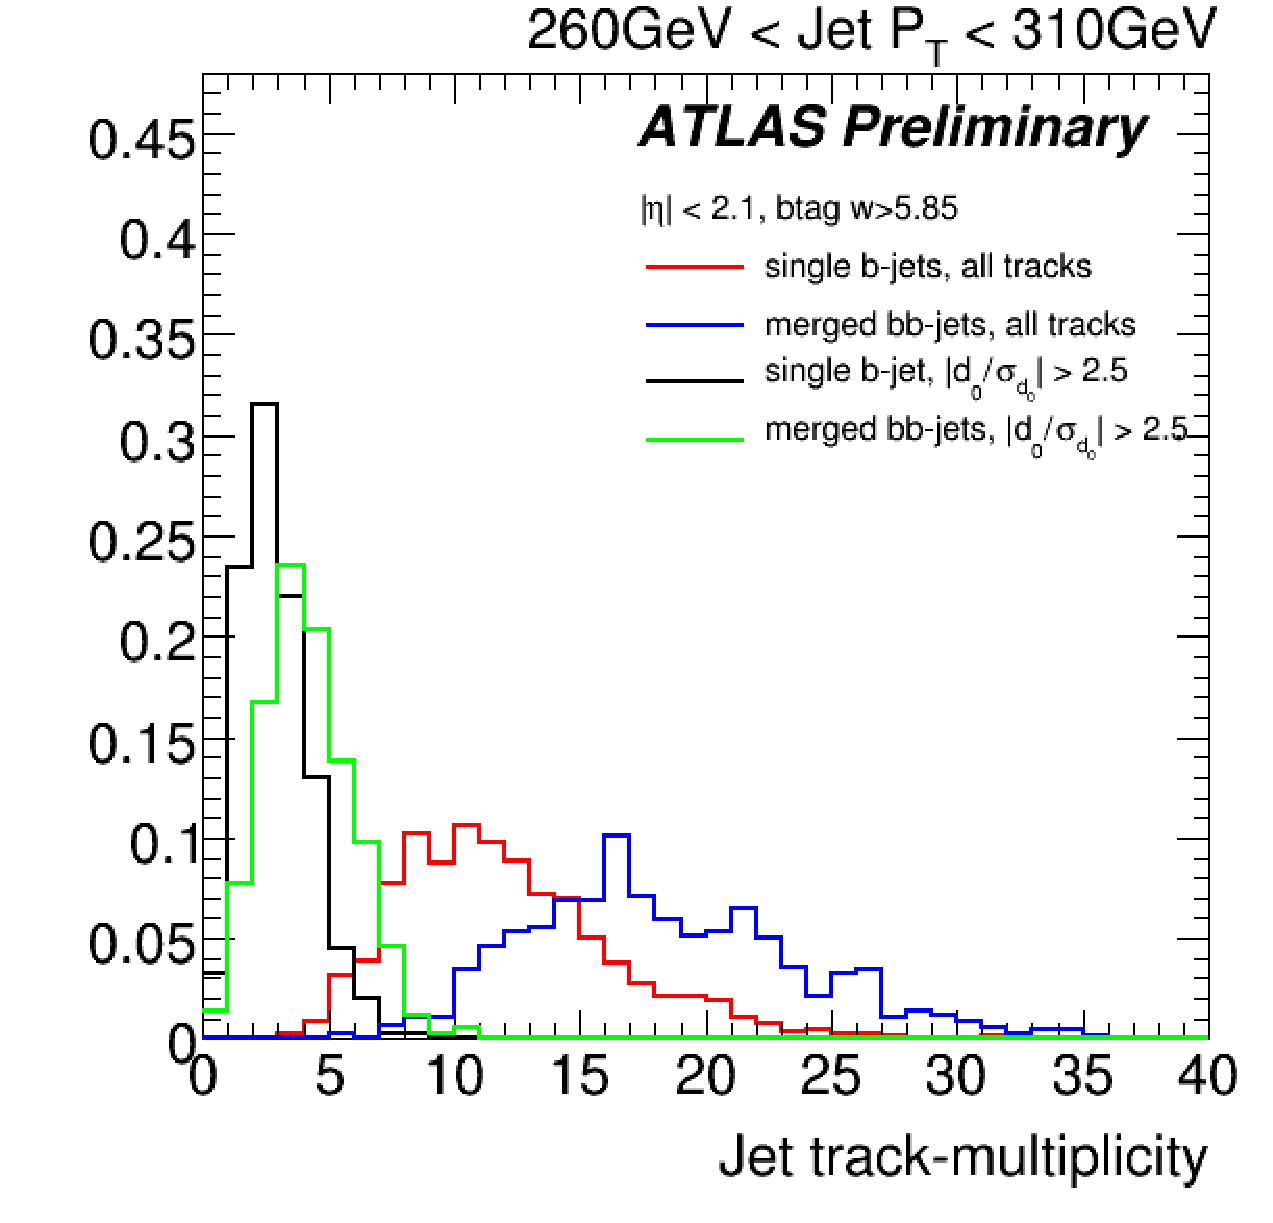
\includegraphics[width=0.49\textwidth]{FIGS/TEMPFigs/DisplacedTracks/ntrk_singlemerged_AllandDisplaced_260-310.pdf}
\caption{Distribution of the jet track multiplicity single and merged $b$-jets between 80~GeV to 110~GeV (left) and 200~GeV to 270~GeV (right), for all and displaced tracks only.}
\label{fig:displacedntrk}
\end{figure}


\begin{figure}[tp]
\centering
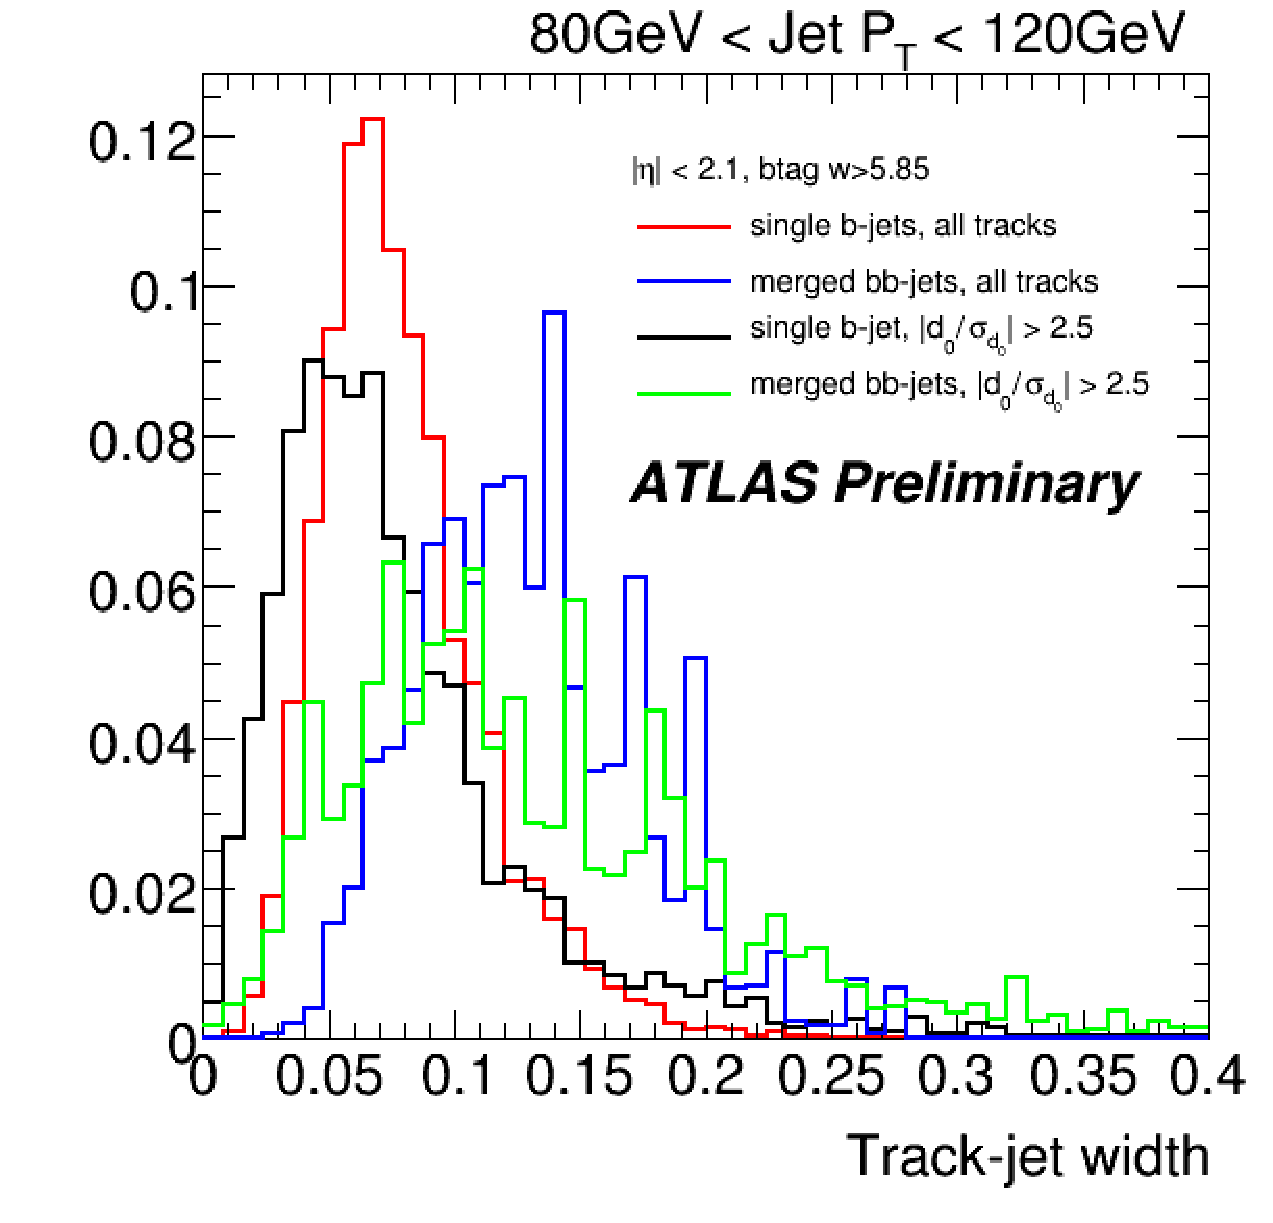
\includegraphics[width=0.49\textwidth]{FIGS/TEMPFigs/DisplacedTracks/trkWidth_singlemerged_AllandDisplaced_80-120.pdf}
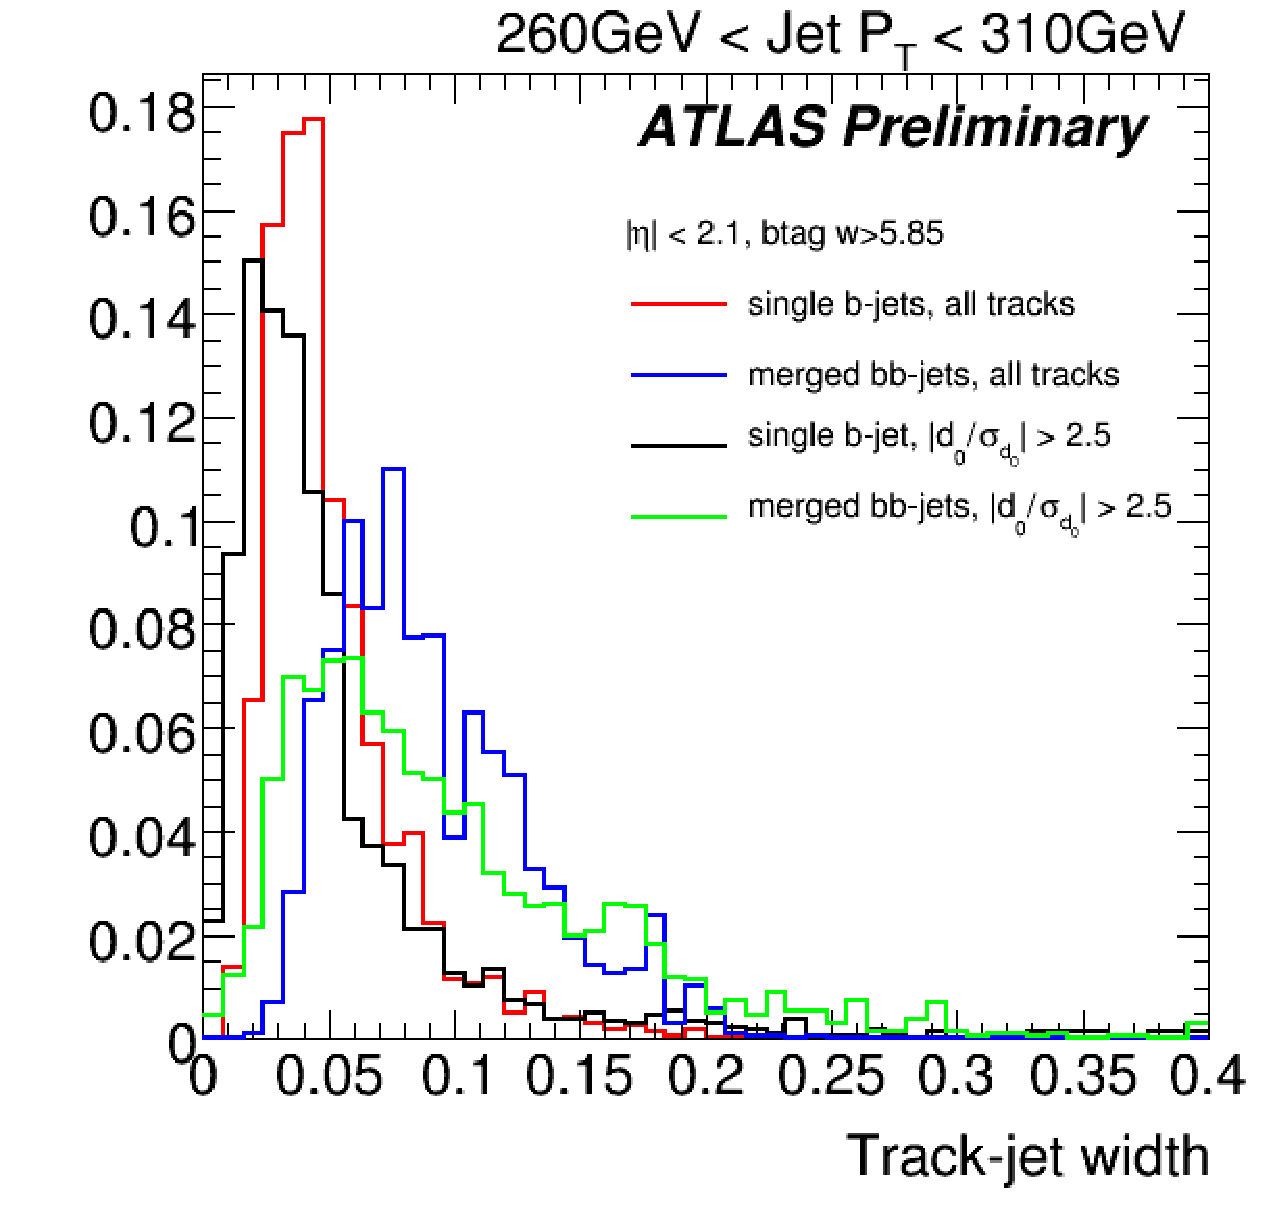
\includegraphics[width=0.49\textwidth]{FIGS/TEMPFigs/DisplacedTracks/trkWidth_singlemerged_AllandDisplaced_260-310.pdf}
\caption{Distribution of the track-jet width for single and merged $b$-jets between 80~GeV to 110~GeV (left) and 200~GeV to 270~GeV (right), for all and displaced tracks only.}
\label{fig:displacedtrkwidth}
\end{figure}


\subsection{Further studies using ``ghost-association'' and bigger cone jets}

In order to better understand the behavior observed for $\tau_2$, $\Delta R$ between the axes of $k_T$ subjets and jet eccentricity in anti-$k_T$ 0.4 jets, these variables were studied for other two different scenarios,

\begin{itemize}\addtolength{\itemsep}{-0.4\baselineskip}
\item 
using the active area of jets (with clusters used as input to jet reconstruction).
\item
using bigger 0.6 anti-$k_T$ jets
\end{itemize}
%
in order to enhance the efficiency to capture the decay products in gluon to $b \bar{b}$-jets.

Figures~\ref{fig:tau2GhostAndAntikt6} to~\ref{fig:jeteccGhostAndAntikt6} show distributions of variables mentioned above for single and merged $b$-jets  between 80~GeV to 110~GeV.

\begin{figure}[tp]
\centering
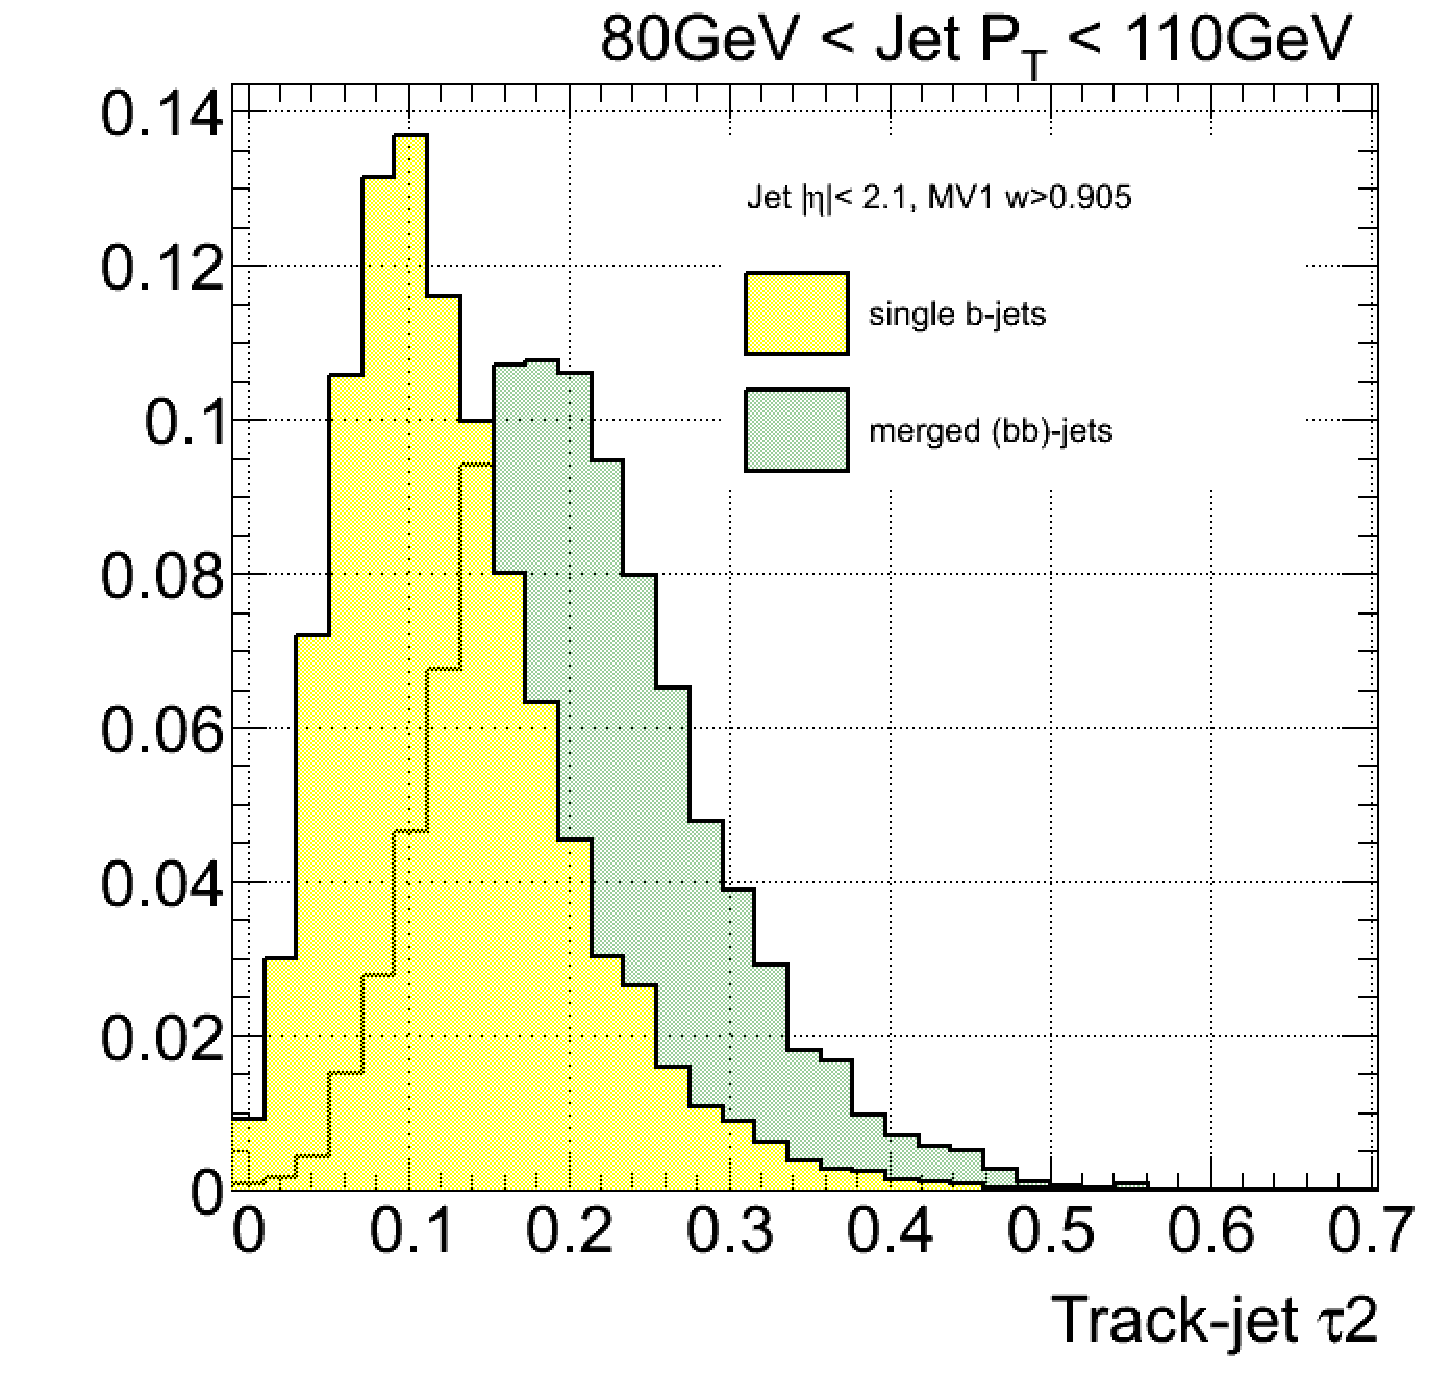
\includegraphics[width=0.49\textwidth]{FIGS/TEMPFigs/Antikt6VarsSingleMerged/Tau2080.pdf}
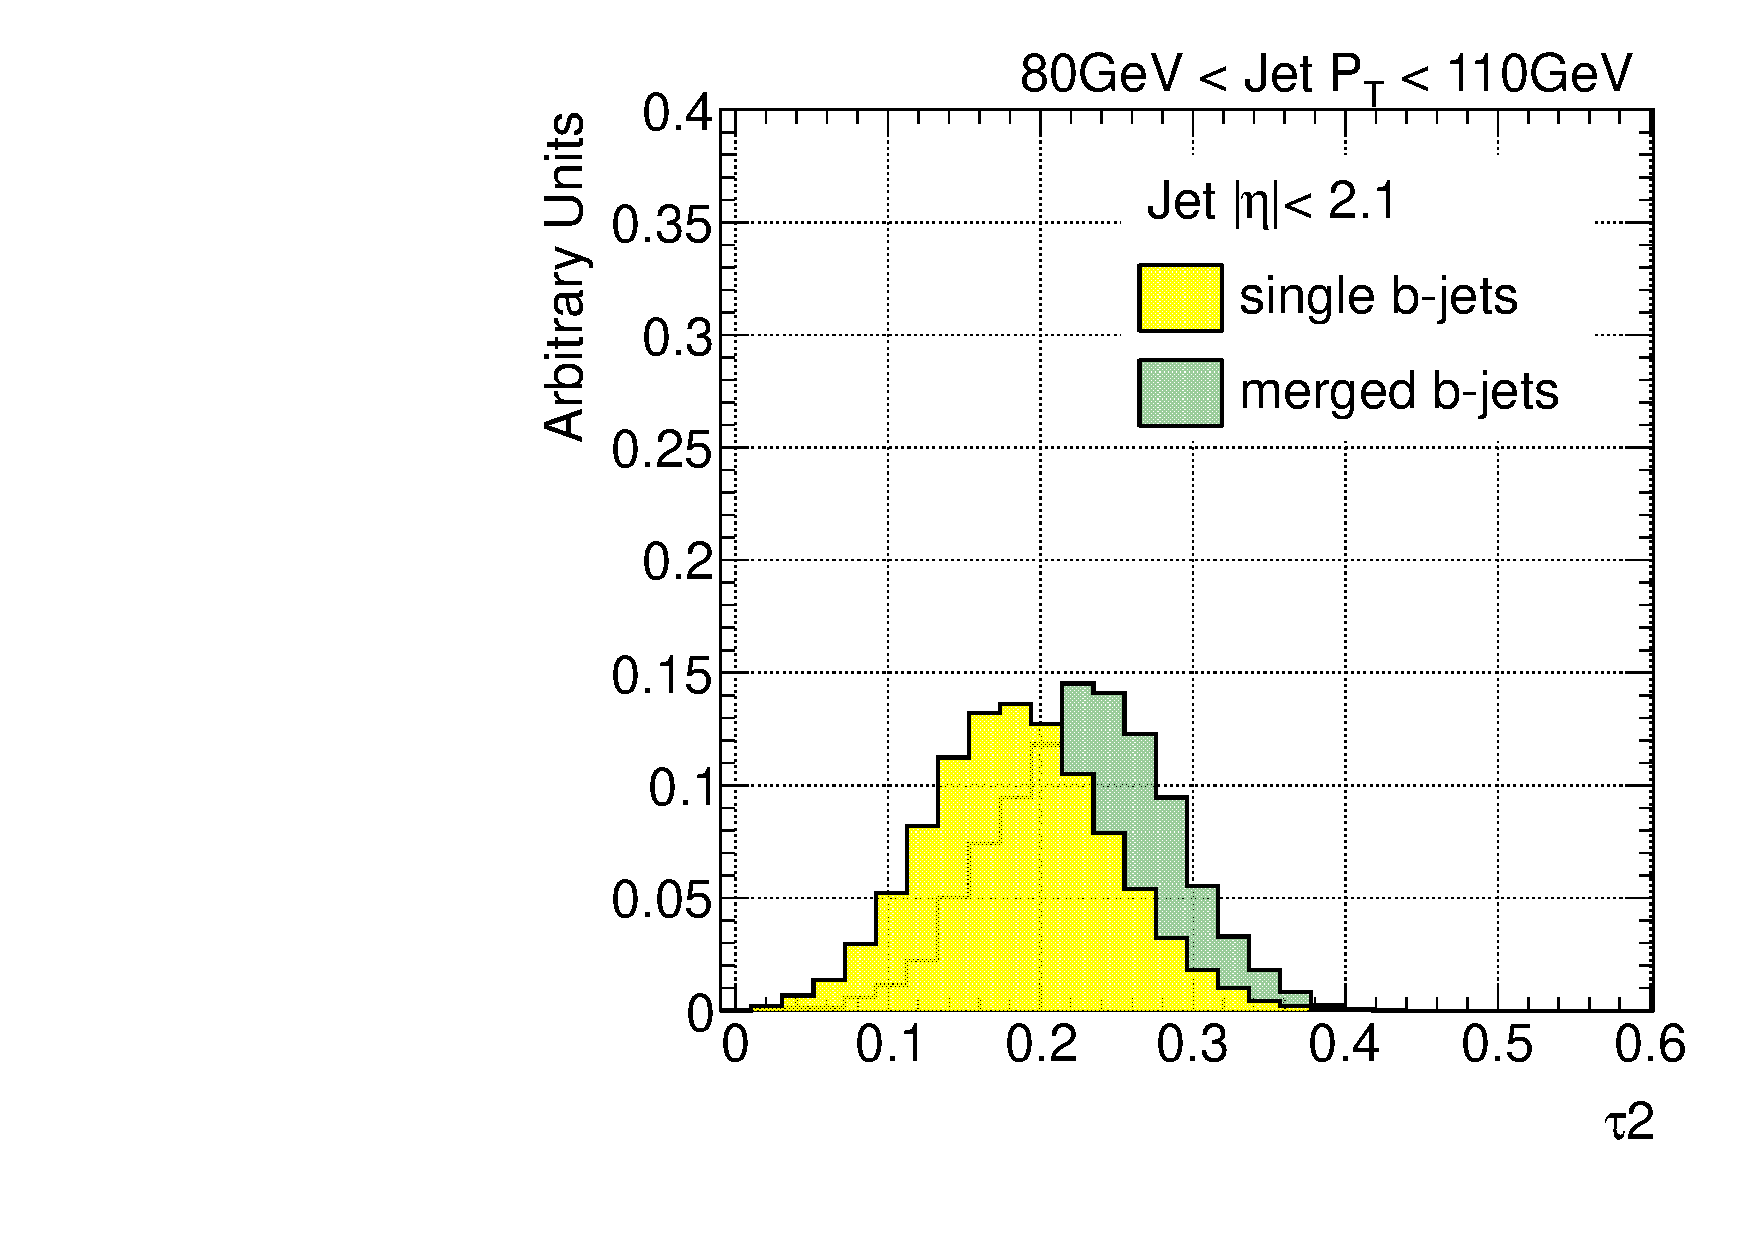
\includegraphics[width=0.49\textwidth]{FIGS/TEMPFigs/GhostMatchingVarsClus/Tau2080.pdf}
\caption{Distribution of $\tau_2$ for single and merged $b$-jets between 80~GeV to 110~GeV in anti-$k_T$ 0.6 jets using track constituents (left) and anti-$k_T$ 0.4 jets using the active area of the jet, with calorimeter topoclusters as input.}
\label{fig:tau2GhostAndAntikt6}
\end{figure}

\begin{figure}[tp]
\centering
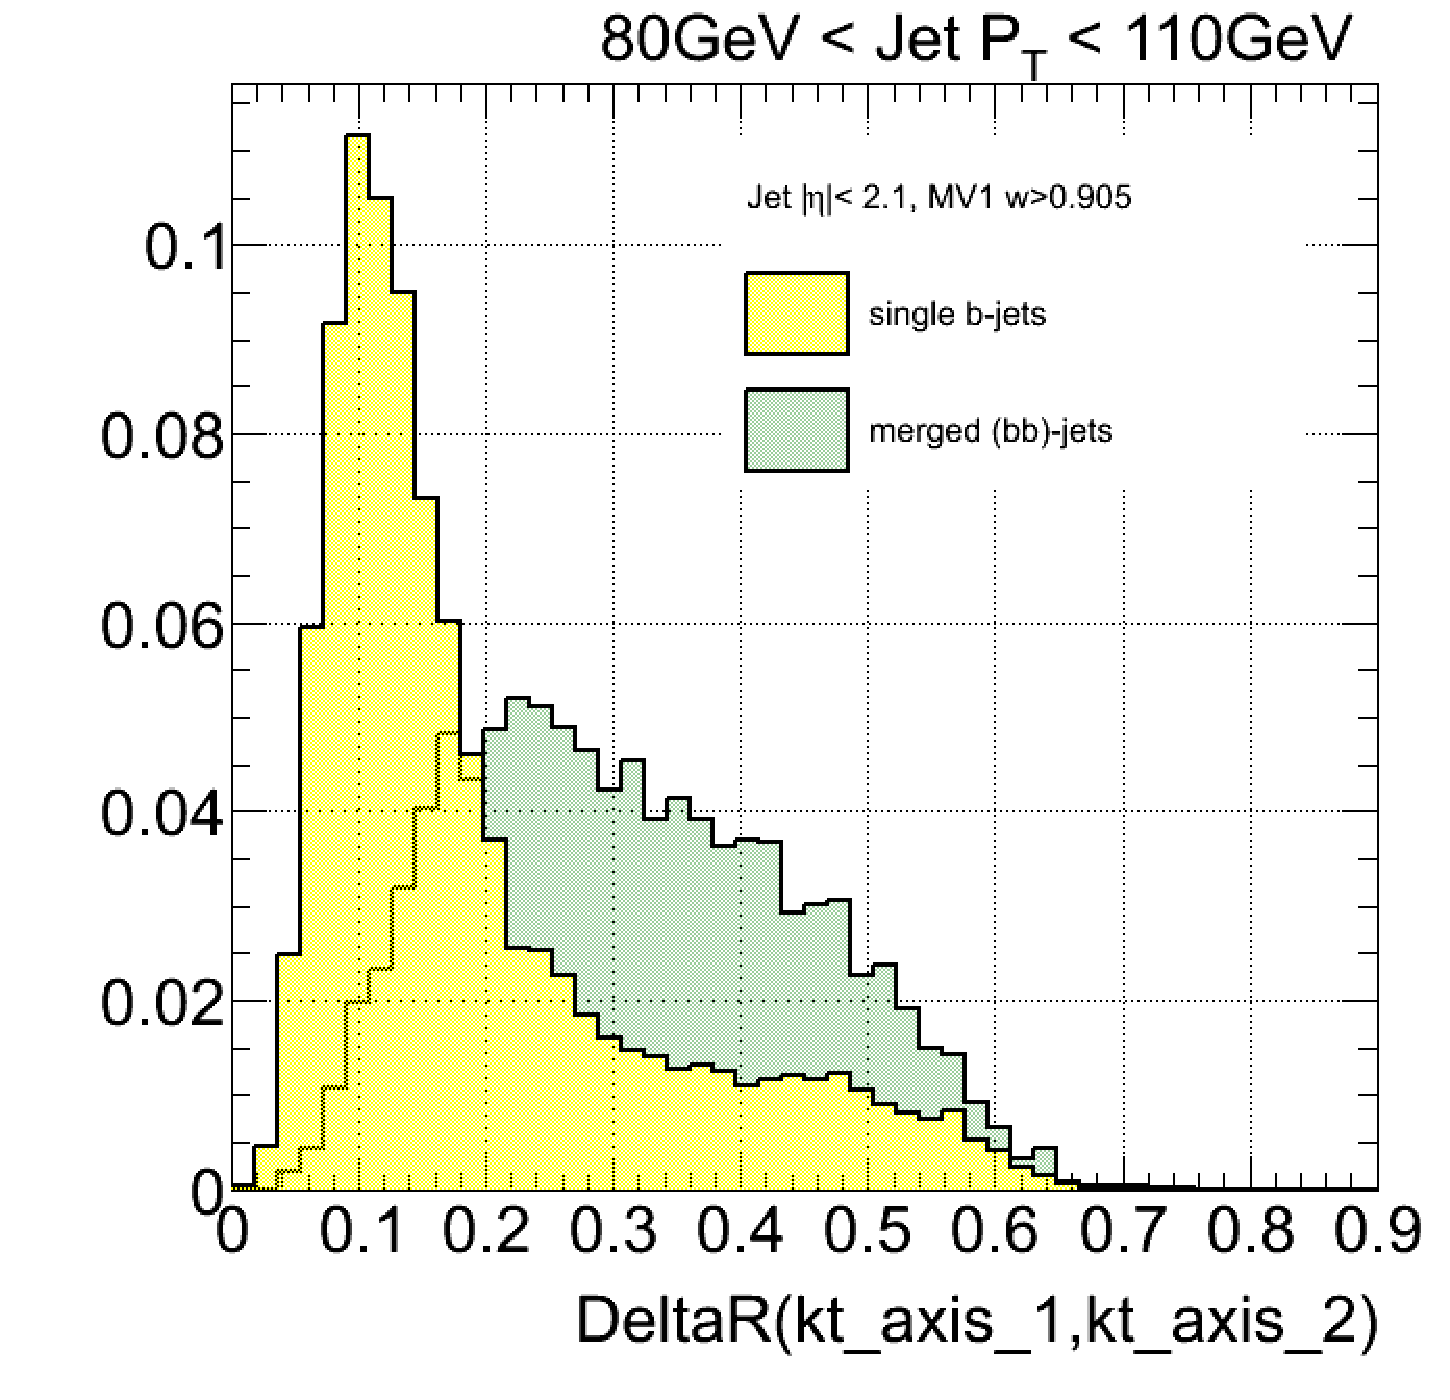
\includegraphics[width=0.49\textwidth]{FIGS/TEMPFigs/Antikt6VarsSingleMerged/DRkt2axes080.pdf}
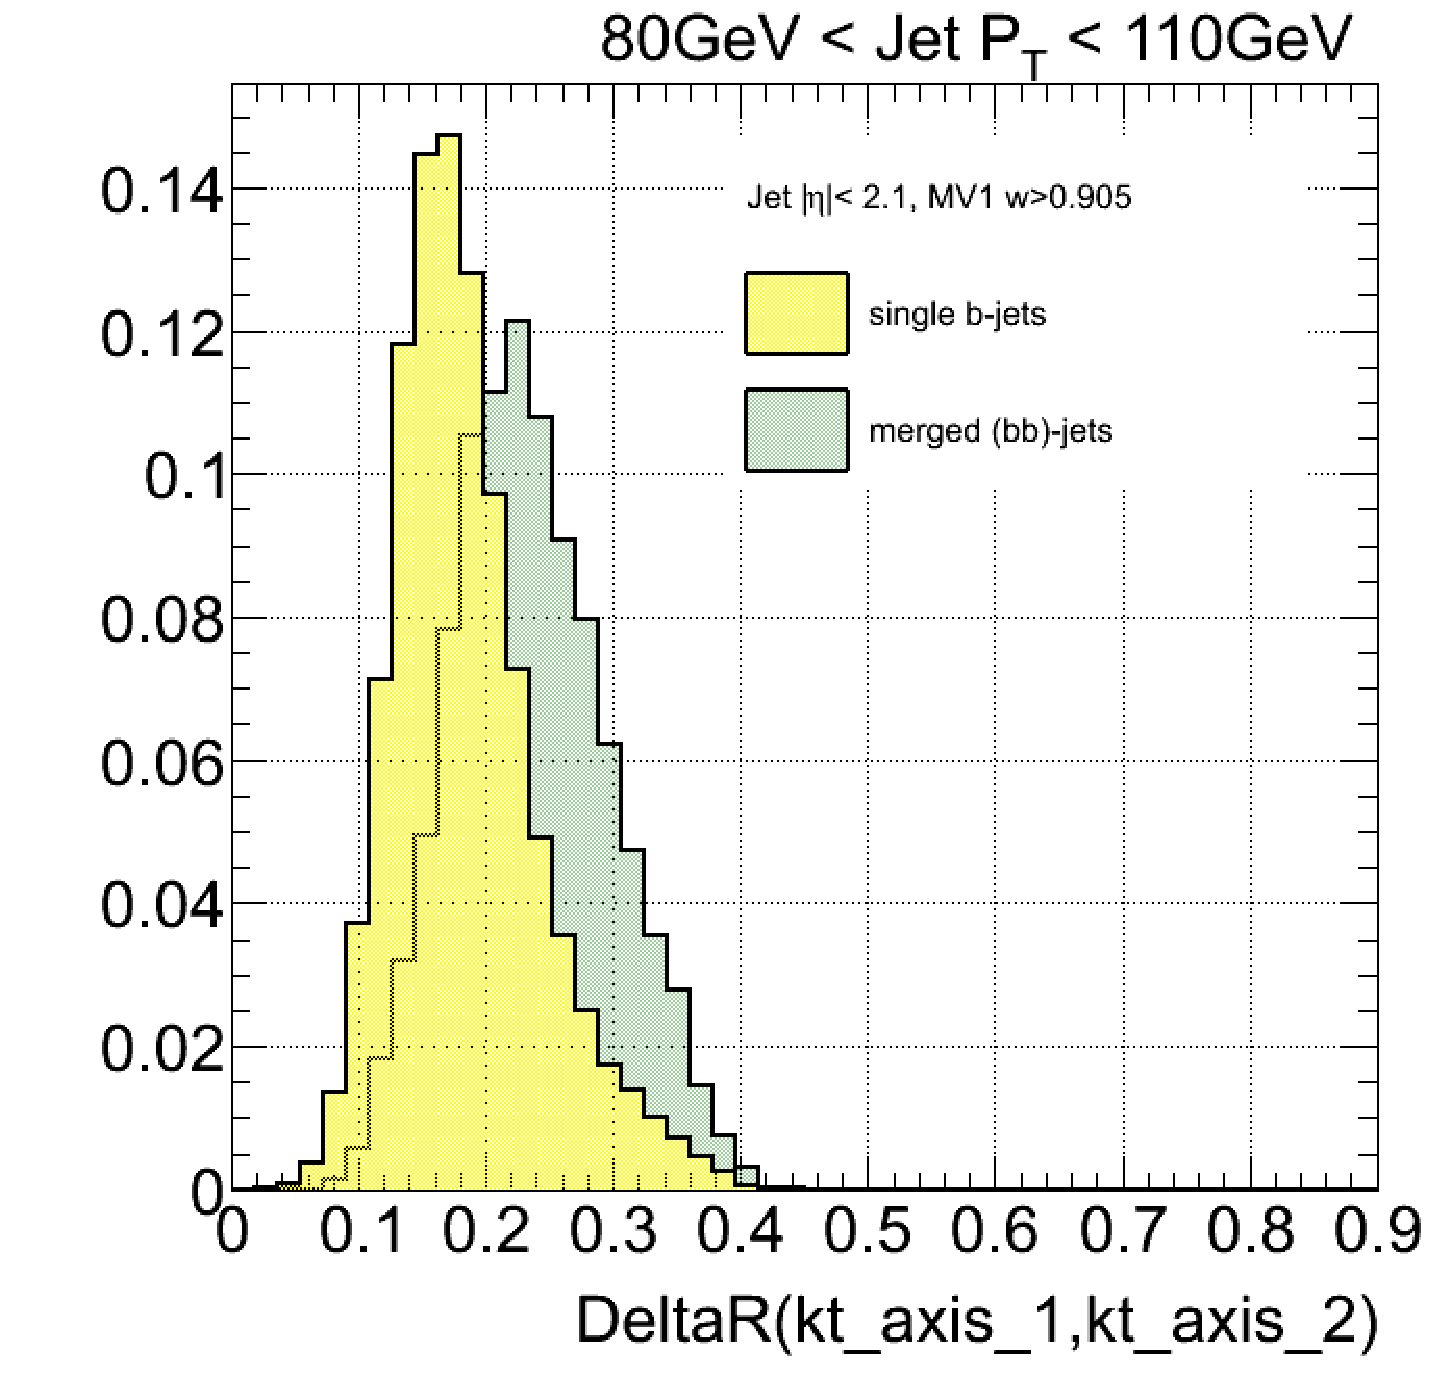
\includegraphics[width=0.49\textwidth]{FIGS/TEMPFigs/GhostMatchingVarsClus/DRkt2axes080.pdf}
\caption{Distribution of $\Delta R$ between $k_T$ subjets for single and merged $b$-jets between 80~GeV to 110~GeV in anti-$k_T$ 0.6 jets using track constituents (left) and anti-$k_T$ 0.4 jets using the active area of the jet, with calorimeter topoclusters as input.}
\label{fig:drktaxisGhostAndAntikt6}
\end{figure}

\begin{figure}[tp]
\centering
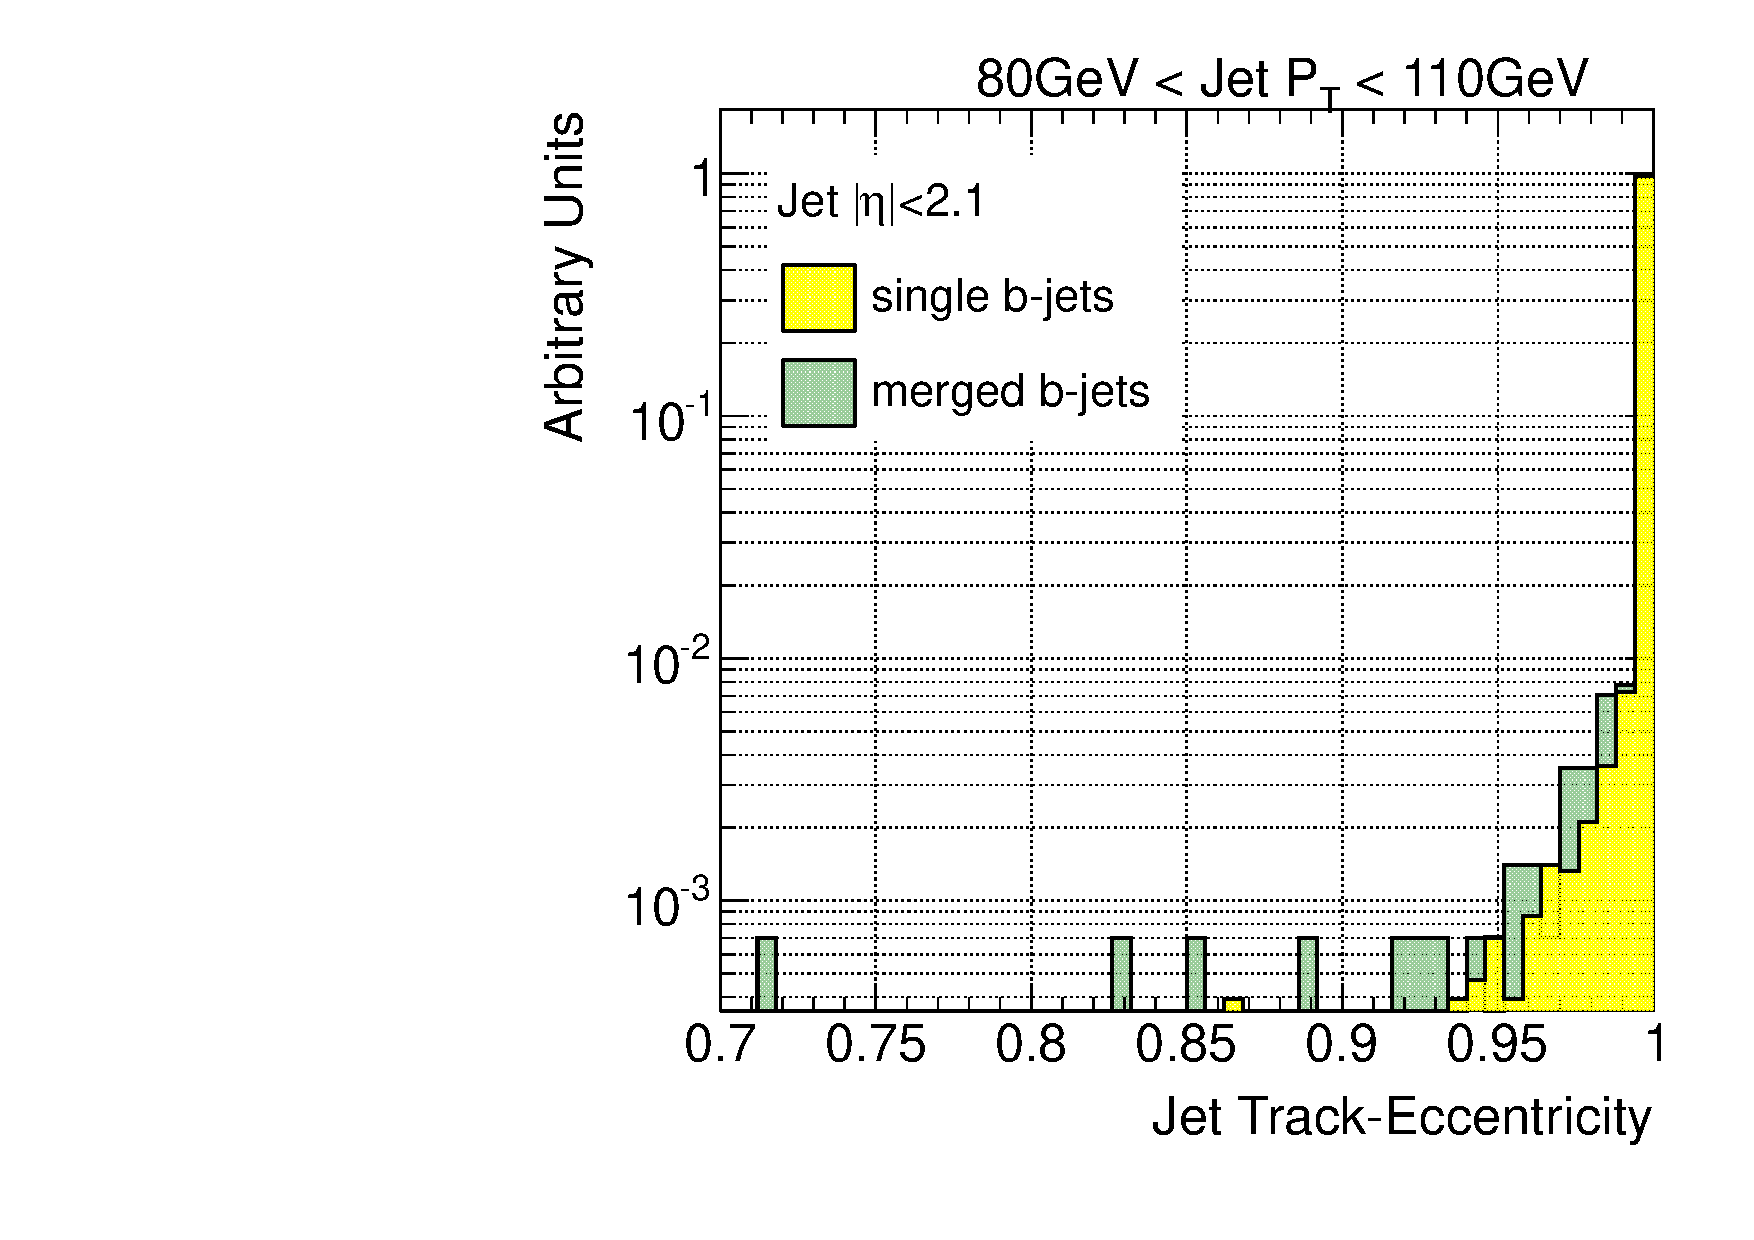
\includegraphics[width=0.49\textwidth]{FIGS/TEMPFigs/Antikt6VarsSingleMerged/JetTrackEccentricity080.pdf}
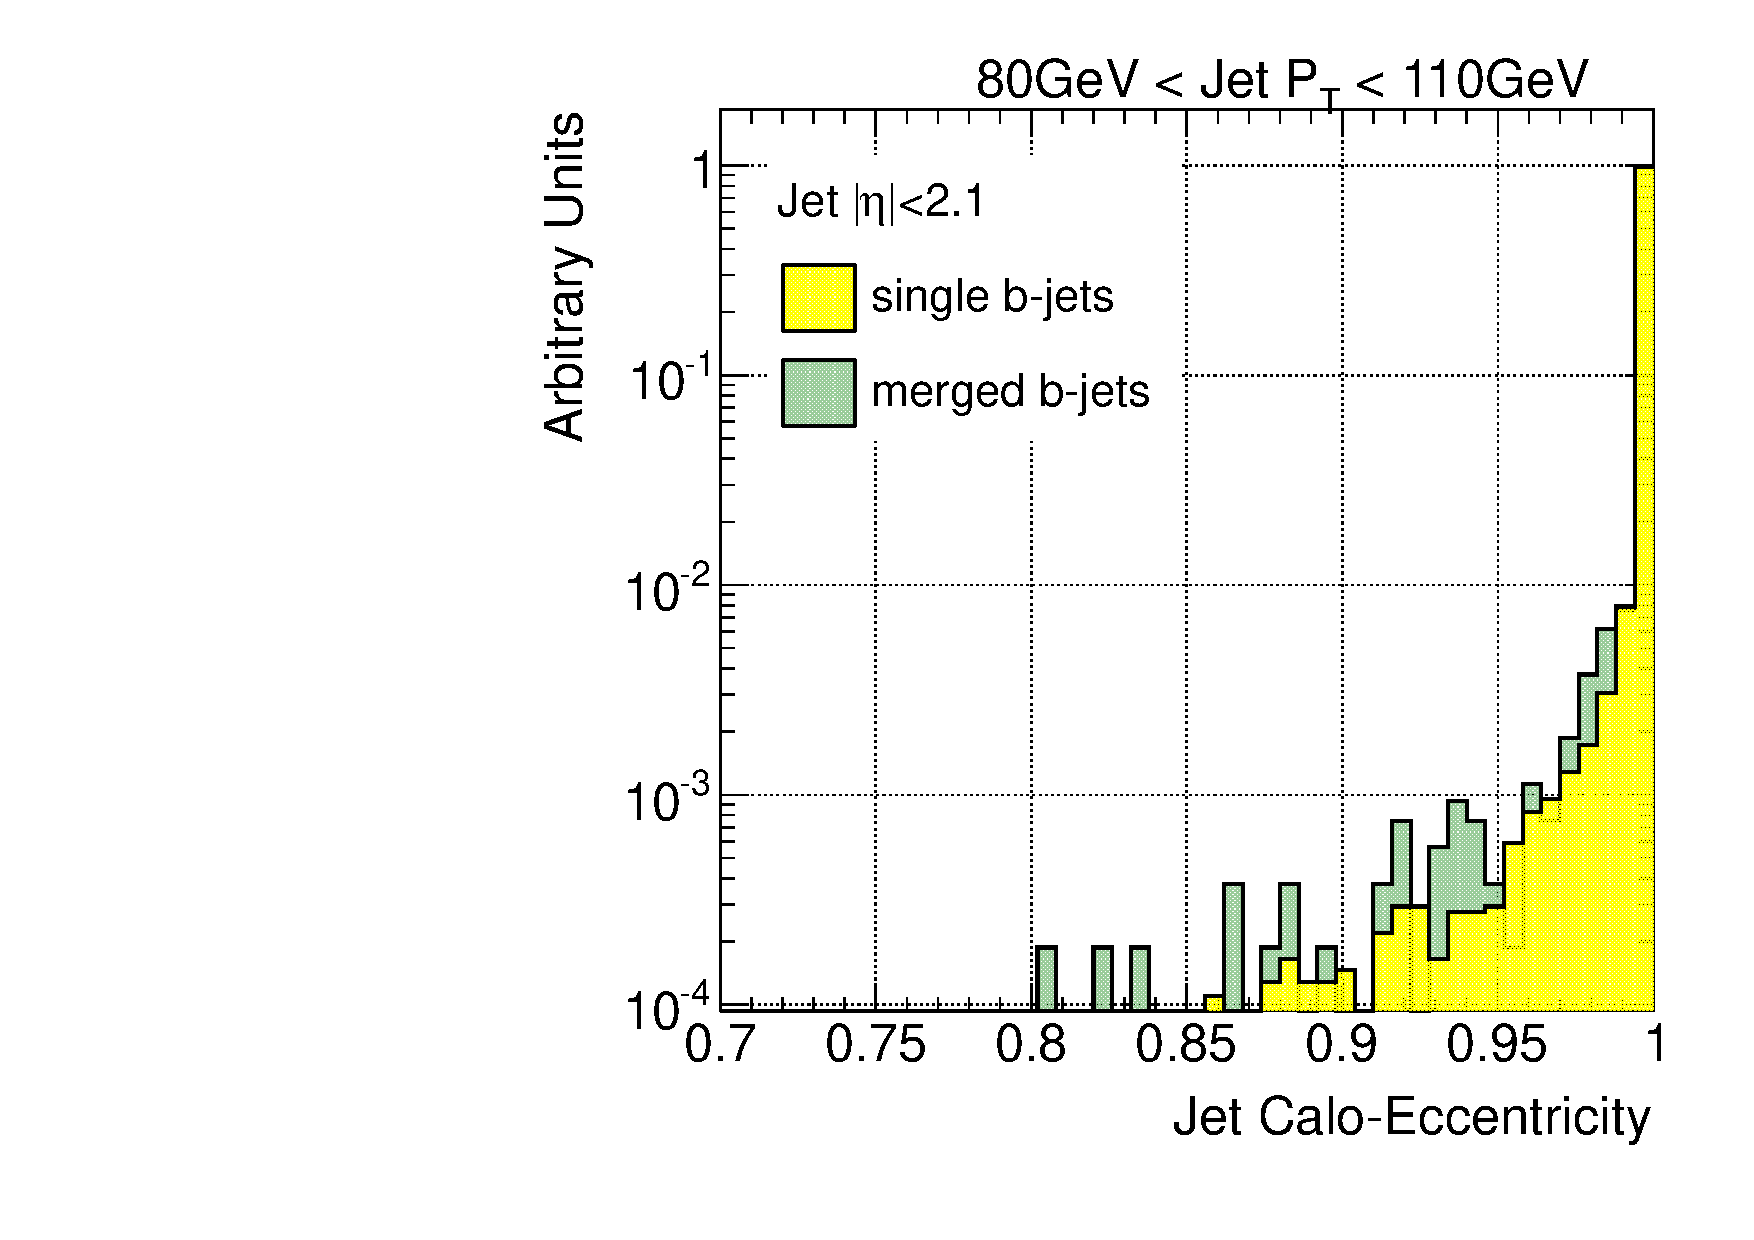
\includegraphics[width=0.49\textwidth]{FIGS/TEMPFigs/GhostMatchingVarsClus/JetCaloEccentricity080.pdf}
\caption{Distribution of the jet eccentricity for single and merged $b$-jets between 80~GeV to 110~GeV in anti-$k_T$ 0.6 jets using track constituents (left) and anti-$k_T$ 0.4 jets using the active area of the jet, with calorimeter topoclusters as input.}
\label{fig:jeteccGhostAndAntikt6}
\end{figure}




%------------------------------------------------------------------------
\section{Validation of the jet variables in data}\label{sec:gbbValidation}
%------------------------------------------------------------------------

 In order to study the extent to which the simulation reproduces the distributions observed in data for the different variables explored a set of comparison plots is presented. Fig.~\ref{fig:datamcinputvars} shows the distributions of jet track multiplicity, track-jet width and $\Delta R$ between the axes of the two $k_t$ subjets, in two different jet $\pt$ bins in dijet Monte Carlo and data events collected by ATLAS %until summer 2011 ($\mu \approx 6$) overlaid.
during 2011. The distributions are normalized to unit area to allow for shape comparisons. There is a good agreement between data and simulation. It should be remarked that the observed agreement is actually not a direct validation of the description in the MC of the relevant variables, but its convolution with the simulated relative fractions of light-, $c$-, $b$- and $bb$-jets in the $b$-tagged generated jet sample. To some extent, some level of compensation can take place between these two effects.

% For the sake of evaluating the effect of the increasing amount of pile-up in the last period of data-taking, %affected the agreement between experimental data and Monte Carlo
%the same distributions were built using data events recorded in the second half of the year ($\mu \approx 12$).  As expected, no significant variation was observed. In Fig.~\ref{fig:datamcinputvarsItoM} the jet track multiplicity is shown for this period, in the same two $\pt$ bins for comparison.  

\begin{figure}[tp]
\centering
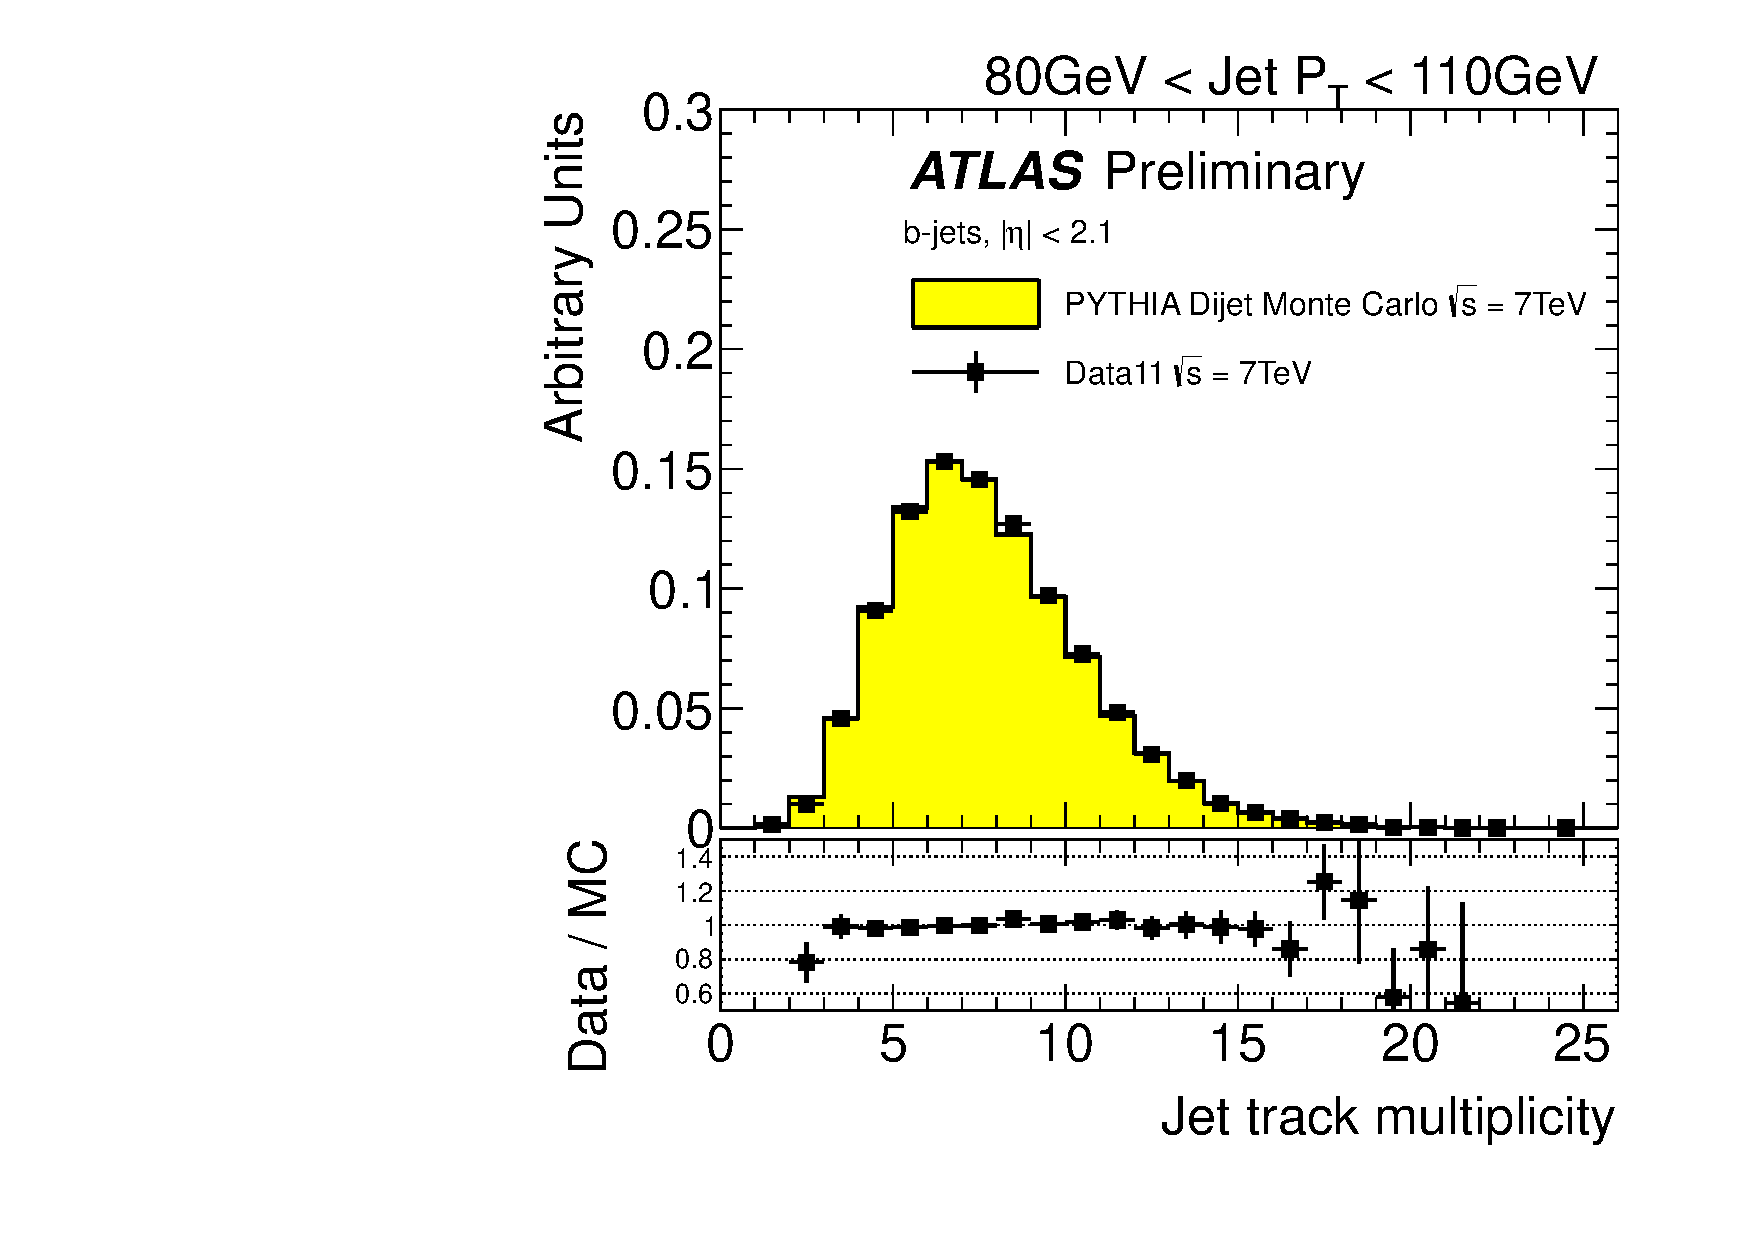
\includegraphics[width=0.49\textwidth]{FIGS/dataMC/FullDataVarNtrkPT080.pdf}
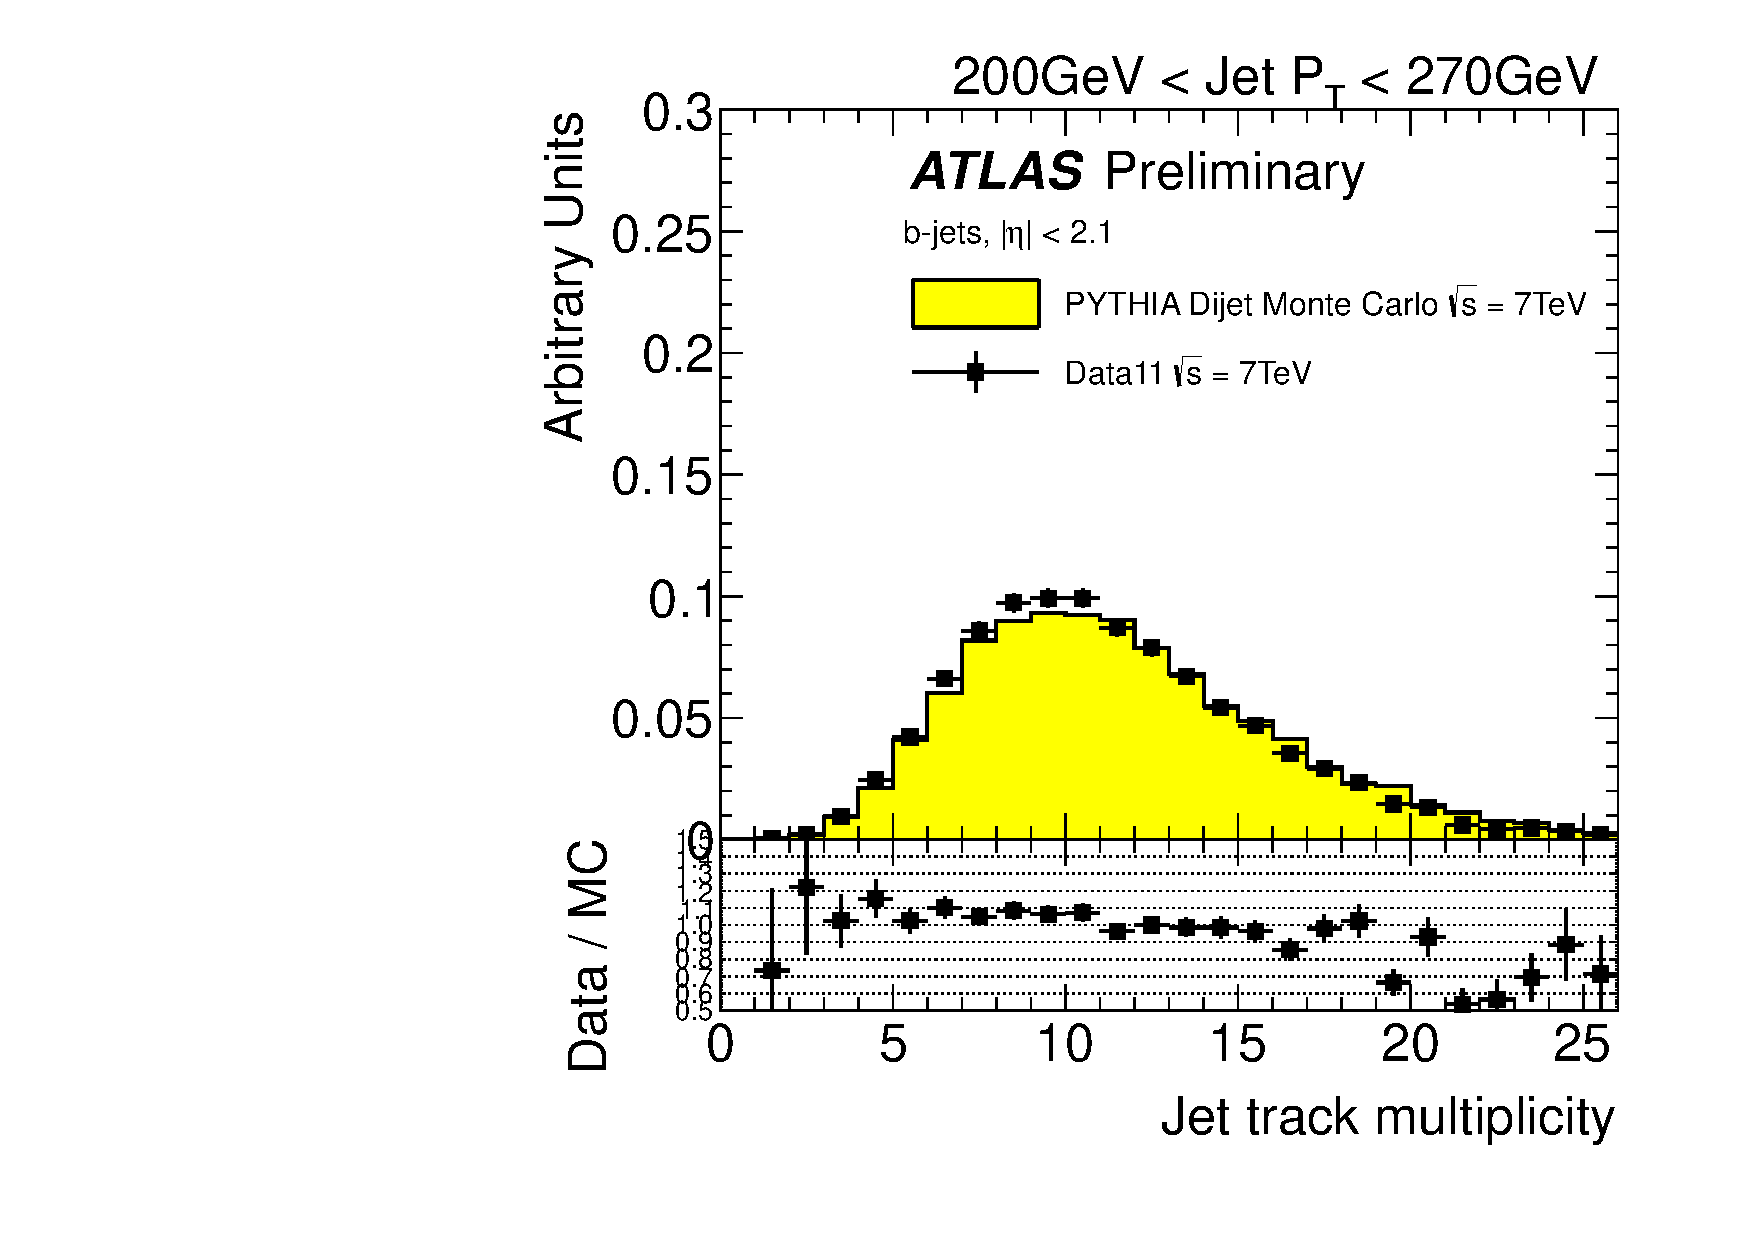
\includegraphics[width=0.49\textwidth]{FIGS/dataMC/FullDataVarNtrkPT200.pdf}
\includegraphics[width=0.49\textwidth]{FIGS/dataMC/FullDataVarTrkWidthPT080.pdf}
\includegraphics[width=0.49\textwidth]{FIGS/dataMC/FullDataVarTrkWidthPT200.pdf}  
\includegraphics[width=0.49\textwidth]{FIGS/dataMC/FullDataVarDRktaxisPT080.pdf}
\includegraphics[width=0.49\textwidth]{FIGS/dataMC/FullDataVarDRktaxisPT200.pdf}  
%\caption{ Distribution of three tracking variables in 2 different jet $\pt$ bins, for experimental data  collected by ATLAS until summer 2011, with $\mu \approx 6$ (solid black points), and simulated data (filled histograms). The ratio data over simulation is shown at the bottom of each plot.}
\caption{ Distribution of three tracking variables in 2 different jet $\pt$ bins, for experimental data  collected by ATLAS during 2011 (solid black points), and simulated data (filled histograms). The ratio data over simulation is shown at the bottom of each plot.}
\label{fig:datamcinputvars}
\end{figure}


%\begin{figure}[tp]
%\centering
%\includegraphics[width=0.49\textwidth]{FIGS/dataMCItoM/VarNtrkPT080.pdf}
%\includegraphics[width=0.49\textwidth]{FIGS/dataMCItoM/VarNtrkPT200.pdf}
%\caption{ Distribution of the jet track-multiplicity in 2 different jet $\pt$ bins, for experimental data from the last period of data-taking, with $\mu \approx 12$ (solid black points), and simulated data (filled histograms). The ratio data over simulation is shown at the bottom of each plot.}
%\label{fig:datamcinputvarsItoM}
%\end{figure}




%
%%%%%%%%%%%%%%%%%%%%%%%%%%%%%%%%%%%%%%%%%%%%%%%%%%%%%%%%%%%%%%%%%%%%%%%%%%%%%%%
% Multivariate Analysis
%%%%%%%%%%%%%%%%%%%%%%%%%%%%%%%%%%%%%%%%%%%%%%%%%%%%%%%%%%%%%%%%%%%%%%%%%%%%%%%
%
\chapter{Multivariate Analysis}\label{chap:mva}


%------------------------------------------------------------------------
\section{The multivariate classifiers}
%------------------------------------------------------------------------

The following multivariate methods were explored:

\begin{itemize}\addtolength{\itemsep}{-0.4\baselineskip}
\item
Likelihood ratio estimators 
\item
Neural Networks (NN)
\item
Boosted decision Trees (BDTs)
\end{itemize}

And different trainings were tested:

\begin{itemize}\addtolength{\itemsep}{-0.4\baselineskip}
\item
Inclusive, with $\pt$-weighting
\item
In bins of jet $\pt$
\end{itemize}


Signal and background jets were not weighted by the dijet samples cross-sections to allow the contribution of subleading lower $\pt$ jets from high $\pt$ events, and thus increase the statistics of merged jets in the low $\pt$ bins. 


Figure~\ref{fig:diffmethodsInclusive} and~\ref{fig:diffmethodsBins} show distributions of the MVA outputs in different bins of jet $\pt$ for the two proposed trainings. In figures~\ref{fig:diffmethodsPerfInclusive} and~\ref{fig:diffmethodsPerfBins} a comparison of the performance of all methods, for inclusive and ``in-bins'', training is illustrated.


\begin{figure}[tp]
\centering
\includegraphics[width=0.32\textwidth]{FIGS/TEMPFigs/MVA_differentMethods/inclusive/NNoutput040_LihoodKDE.pdf}
\includegraphics[width=0.32\textwidth]{FIGS/TEMPFigs/MVA_differentMethods/inclusive/NNoutput080_LihoodKDE.pdf}
\includegraphics[width=0.32\textwidth]{FIGS/TEMPFigs/MVA_differentMethods/inclusive/NNoutput200_LihoodKDE.pdf}
\includegraphics[width=0.32\textwidth]{FIGS/TEMPFigs/MVA_differentMethods/inclusive/NNoutput040_MLP.pdf}
\includegraphics[width=0.32\textwidth]{FIGS/TEMPFigs/MVA_differentMethods/inclusive/NNoutput080_MLP.pdf}
\includegraphics[width=0.32\textwidth]{FIGS/TEMPFigs/MVA_differentMethods/inclusive/NNoutput200_MLP.pdf}
\includegraphics[width=0.32\textwidth]{FIGS/TEMPFigs/MVA_differentMethods/inclusive/NNoutput040_BDT.pdf}
\includegraphics[width=0.32\textwidth]{FIGS/TEMPFigs/MVA_differentMethods/inclusive/NNoutput080_BDT.pdf}
\includegraphics[width=0.32\textwidth]{FIGS/TEMPFigs/MVA_differentMethods/inclusive/NNoutput200_BDT.pdf}
\caption{Distribution of the MVA discriminant outputs, for inclusive training, in single and merged $b$-jets, for low, medium and high jet $\pt$.}
\label{fig:diffmethodsInclusive}
\end{figure}

\begin{figure}[tp]
\centering
\includegraphics[width=0.32\textwidth]{FIGS/TEMPFigs/MVA_differentMethods/bins/NNoutput040_LihoodKDE.pdf}
\includegraphics[width=0.32\textwidth]{FIGS/TEMPFigs/MVA_differentMethods/bins/NNoutput080_LihoodKDE.pdf}
\includegraphics[width=0.32\textwidth]{FIGS/TEMPFigs/MVA_differentMethods/bins/NNoutput200_LihoodKDE.pdf}
\includegraphics[width=0.32\textwidth]{FIGS/TEMPFigs/MVA_differentMethods/bins/NNoutput040_MLP.pdf}
\includegraphics[width=0.32\textwidth]{FIGS/TEMPFigs/MVA_differentMethods/bins/NNoutput080_MLP.pdf}
\includegraphics[width=0.32\textwidth]{FIGS/TEMPFigs/MVA_differentMethods/bins/NNoutput200_MLP.pdf}
\includegraphics[width=0.32\textwidth]{FIGS/TEMPFigs/MVA_differentMethods/bins/NNoutput040_BDT.pdf}
\includegraphics[width=0.32\textwidth]{FIGS/TEMPFigs/MVA_differentMethods/bins/NNoutput080_BDT.pdf}
\includegraphics[width=0.32\textwidth]{FIGS/TEMPFigs/MVA_differentMethods/bins/NNoutput200_BDT.pdf}
\caption{Distribution of the MVA discriminant outputs, for training in bins of jet $\pt$, in single and merged $b$-jets, for low, medium and high jet $\pt$.}
\label{fig:diffmethodsBins}
\end{figure}

\begin{figure}[tp]
\centering
\includegraphics[width=0.49\textwidth]{FIGS/TEMPFigs/MVA_differentMethods/inclusive/MVAs_RejvsEff40.pdf}
\includegraphics[width=0.49\textwidth]{FIGS/TEMPFigs/MVA_differentMethods/inclusive/MVAs_RejvsEff200.pdf}
\caption{Distribution of the MVA discriminant performance for inclusive training, in single and merged $b$-jets, for low and high jet $\pt$.}
\label{fig:diffmethodsPerfInclusive}
\end{figure}

\begin{figure}[tp]
\centering
\includegraphics[width=0.49\textwidth]{FIGS/TEMPFigs/MVA_differentMethods/bins/MVAs_RejvsEff40.pdf}
\includegraphics[width=0.49\textwidth]{FIGS/TEMPFigs/MVA_differentMethods/bins/MVAs_RejvsEff200.pdf}
\caption{Distribution of the MVA discriminant performance for training in bins of jet $\pt$, in single and merged $b$-jets, for low and high jet $\pt$.}
\label{fig:diffmethodsPerfBins}
\end{figure}

%------------------------------------------------------------------------
\section{The input variables}
%------------------------------------------------------------------------

Different groups of input variables were tested. Figure~\ref{fig:difftrainings} shows the performance for three sets of variables for MVA classifier.

\begin{figure}[tp]
\centering
\includegraphics[width=0.32\textwidth]{FIGS/TEMPFigs/MVA_differentTrainings/DiffTrainings_RejvsEff40.pdf}
\includegraphics[width=0.32\textwidth]{FIGS/TEMPFigs/MVA_differentTrainings/DiffTrainings_RejvsEff80.pdf}
\includegraphics[width=0.32\textwidth]{FIGS/TEMPFigs/MVA_differentTrainings/DiffTrainings_RejvsEff200.pdf}
\caption{Distribution of the MVA discriminant performance for three sets of input variables, in single and merged $b$-jets, for low, medium and high jet $\pt$.}
\label{fig:outputinbin}
\end{figure}

%------------------------------------------------------------------------
\section{$\bm{ g\rightarrow b\bar{b}}$ likelihood training and performance}
%------------------------------------------------------------------------

A discriminant between single $b$-jets and merged $b$-jets was built by training a simple likelihood estimator in the context of the Toolkit for Multivariate Data Analysis, TMVA~\cite{Hocker:2007ht}.

A sub-set of the dijet Monte Carlo sample was used for training. After the event and jet selections were performed, the $b$-tagged jets with $|\eta| < 2.1$ were classified as signal (single $b$-jets) or background (merged $b$). % depending on whether one or two $B$-hadrons were found within a 0.4 cone around the jet axis. %For the evaluation of the method the same procedure was followed.
The likelihood training was done in bins of calorimeter jet $\pt$. % and only isolated jets were considered. 
Signal and background jets were not weighted by the dijet samples cross-sections to allow the contribution of subleading lower $\pt$ jets from high $\pt$ events, and thus increase the statistics of merged jets in the low $\pt$ bins. For the evaluation of the method the same procedure was followed.

Several combinations of the tracking and jet shape variables studied in the previous section were tested as input variables. We found that the following three offer the best performance:
% that the jet track multiplicity, the track-jet width and $\Delta R$  between the axes of the two $k_t$ subjets offered the best performance. 
\begin{enumerate}\addtolength{\itemsep}{-0.4\baselineskip}
\item
Jet track multiplicity
\item
Track-jet width
\item
$\Delta R$ between the axes of 2 $k_t$ subjets within the jet
\end{enumerate}
%
A requirement of at least two matching tracks was imposed to all $b$-tagged jets in order to build the third variable listed. This cut was applied in both training and testing samples.

The distribution of the likelihood output for single and merged $b$-jets is shown in  Fig.~\ref{fig:outputinbins} for low, medium and high transverse momentum jets.

\begin{figure}[tp]
\centering
\includegraphics[width=0.32\textwidth,viewport=40 0 540 550]{FIGS/Likelihood/NNoutput040_LihoodKDE.pdf}
%\includegraphics[width=0.32\textwidth]{FIGS/Likelihood/NNoutput040_LihoodKDE.pdf}
\includegraphics[width=0.32\textwidth,viewport=40 0 540 550,clip]{FIGS/Likelihood/NNoutput080_LihoodKDE.pdf}
\includegraphics[width=0.32\textwidth,viewport=40 0 540 550,clip]{FIGS/Likelihood/NNoutput200_LihoodKDE.pdf}  
\caption{Distribution of the $g\rightarrow b \bar{b}$ likelihood output for single and merged $b$-jets for low, medium and high $\pt$ jets.}
\label{fig:outputinbins}
\end{figure}

The performance of the $g\rightarrow b \bar{b}$ tagger in the simulation can be  %seen in Fig.~\ref{fig:performanceinbins}. In this plot the rejection ($1/\epsilon_{bkg}$) of merged $b$-jets from gluon splitting is shown as a function of single $b$-jet efficiency for the eight bins of jet $\pt$ mentioned in section~\ref{sec:EventSelection}. The performance improves with $\pt$:
displayed in a plot of rejection ($1/\epsilon_{bkg}$) of merged $b$-jets as a function of single $b$-jet efficiency, where $\epsilon_{bkg}$ is the probability that a $b \bar{b}$-jet passes the tagger. This is shown in Fig.~\ref{fig:performanceinbins} for the eight bins of jet $\pt$ mentioned in section~\ref{sec:EventSelection}. The performance improves with $\pt$:


\begin{itemize}\addtolength{\itemsep}{-0.4\baselineskip}
\item
$\pt>40$ GeV: %\\[1mm]
rejection above 8 at 50\% eff.
% over 85\% rejection at 50\% eff.
\item
$\pt>60$ GeV: %\\[1mm]
rejection above 10 at 50\% eff.
 %90\% rejection at 50\% eff.
\item
$\pt>200$ GeV: %\\[1mm]
rejection above 30 at 50\% eff.
 %over 95\% rejection at 50\% eff.
\end{itemize}


\begin{figure}[tp]
\centering
\includegraphics[width=0.7\textwidth]{FIGS/Likelihood/KDE_RejvsEff.pdf}
\caption{Rejection of $g\rightarrow b \bar{b}$ merged $b$-jets as a function of $b$-jet efficiency for dijet events in 8 jet $\pt$ bins.}
\label{fig:performanceinbins}
\end{figure}

The likelihood was trained with jets that had been first tagged by the MV1 algorithm. In order to use the  $g\rightarrow b \bar{b}$ classifier for jets tagged by another tagger a new training is required.

The rejection of merged jets attained as a function of $\pt$ for the 50\% and 60\% efficiency working points are summarized in Table~\ref{tb:rejection}, together with their relative statistical error. These are propagated from the Poisson fluctuations of the number of events in the merged and single $b\bar{b}$ distributions. The error is slightly lower for the 60\% efficiency working point because a higher efficiency allows for a greater number of Monte Carlo events to measure the performance. %the higher the efficiency, the larger the number of Monte Carlo events available to measure the performance.



\begin{table}[!hbt] %[h]
\renewcommand{\arraystretch}{1.2}
\centering
\begin{tabular}{ | c || c | c || c | c||}
  \hline
  Jet $\pt$ & \multicolumn{2}{c||}{single $b$-jet efficiency 50\%} & 
            \multicolumn{2}{c||}{single $b$-jet efficiency 60\%}\\ \cline{2-5}
    (GeV )  & Rejection & ~stat.err.~ & Rejection & ~stat.err.~ \\ \hline
%   40 - 60 &  ~7.6 &  4\%  &  ~5.4  &  3\%    \\ 
%   60 - 80 &  10.4 &  4\%  &  ~7.3  &  4\%    \\ 
%   80 - 110&  13.9 &  5\%  &  ~9.4  &  4\%    \\ 
%  110 - 150&  18.7 &  5\%  &  12.0  &  4\%    \\ 
%  150 - 200&  23.2 &  5\%  &  14.0  &  5\%    \\ 
%  200 - 270&  29.5 &  7\%  &  15.6  &  6\%    \\ 
%  270 - 360&  36.4 &  7\%  &  18.7  &  6\%    \\ 
%  360 - 480&  41.4 &  8\%  &  18.2  &  8\%    \\ \hline
   40 - 60 &  ~8 &  4\%  &  ~5  &  3\%    \\ 
   60 - 80 &  ~10 &  4\%  &  ~7  &  4\%    \\ 
   80 - 110&  ~14 &  5\%  &  ~9  &  4\%    \\ 
  110 - 150&  19 &  5\%  &  12  &  4\%    \\ 
  150 - 200&  23 &  5\%  &  14  &  5\%    \\ 
  200 - 270&  30 &  7\%  &  16  &  6\%    \\ 
  270 - 360&  36 &  7\%  &  19  &  6\%    \\ 
  360 - 480&  41 &  8\%  &  18  &  8\%    \\ \hline
\end{tabular}
\caption{The merged $b$-jet rejection for the 50\% and 60\% efficiency working points in bins of $\pt$.}
\label{tb:rejection}
\end{table}







%------------------------------------------------------------------------
\section{Systematic uncertainties}\label{sec:gbbSystematics}
%------------------------------------------------------------------------

The development, training and performance determination of the tagger is based on simulated events. Although the agreement between simulation and data explored in section~\ref{sec:validation} is a necessary validation condition, it is also important to investigate how the tagger performance depends on systematics relevant in the data. In particular we have considered:
%
%There are uncertainties in the data that, although not spoiling the data/MC agreement, might change the performance of the tagger. This uncertainties would also be present in an eventual future data-driven determination of the performance as  the data are not known better that this.The following systematic effects have been studied and their influence on the tagger performance ascertained:
%
%In order to study the systematic uncertainties in the method the following contributions were evaluated:
\begin{itemize}\addtolength{\itemsep}{-0.4\baselineskip}
\item
presence of additional interactions (pile-up)
\item
uncertainty in the $b$-jet tagging efficiency % and b-jet energy scale?
\item
uncertainty in the track reconstruction efficiency
\item
uncertainty in the track transverse momentum resolution
\item
uncertainty in the jet transverse momentum resolution  
%\item
%the effect of jet isolation
%\item
%other $\Delta R$ cuts for B-labeling and matching
\end{itemize}

{ \em I. Pile-up}
\\[3mm]
  The size of this effect was studied by comparing the performance of the likelihood discriminant with $b$-jets in events with small (1-9) and large (9-20) number of primary vertices. 
The comparison of the performance in these two sub-samples can be seen in Fig.~\ref{fig:performanceinbinsMu}. 
As expected from the use of tracking (as opposed to calorimeter) variables no significant dependence with pile-up is observed within statistics. Of the 16 determinations (2 working points with 8 $\pt$ bins each) of performance differences between high and low number of primary vertices events, it is observed that 6 of them are positive and 10 negative, with a global mean of 0.3\%. We conclude that the effect is negligible compared to other source of uncertainties.
%

\begin{figure}[tp]
\centering
\includegraphics[width=0.49\textwidth]{FIGS/systematics/50BinsLlhoodKDE_ISO_PileUp_rejvseff040.pdf}
\includegraphics[width=0.49\textwidth]{FIGS/systematics/50BinsLlhoodKDE_ISO_PileUp_rejvseff060.pdf}
\caption{Rejection of $g\rightarrow b \bar{b}$ merged b-jets as a function of $b$-jet efficiency in bins of $N_{\rm vtx}$ for two low jet $\pt$ bins.}
\label{fig:performanceinbinsMu}
\end{figure}

\vspace{3mm}
{\em II. b-tagging efficiency} %energy scale and 
\\[3mm]
The performance of heavy-flavor tagging in Monte Carlo events is calibrated to experimental data by means of the scale factors (SFs) measured by the $b$-tagging group. %scale factors defined as the ratio of the heavy-flavor tagging efficiency in data over that in Monte Carlo (MC) for the different jet flavors, and probably also as a function of jet pT and η 
Such a measurement carries a systematic uncertainty, and in order to estimate its effect a conservative approach is followed: %https://twiki.cern.ch/twiki/bin/viewauth/AtlasProtected/BTaggingCalibrationDataInterface
the SFs are varied in all the $\pt$ bins simultaneously by one standard deviation both in the up and down directions. The result of this procedure for the distribution of two of the tracking variables used in our discriminant is illustrated in Fig.~\ref{fig:btaggingSFs}. 

The effect of the $b$-tagging calibration uncertainty on the likelihood peformance is $< 1$\%, negligible with respect to the statistical uncertainty as it can be seen in Fig.~\ref{fig:btaggingSFsPerf}.
This was indeed expected. The scale factors depend on the true flavor of the jet and on its $\pt$, but these are basically constant in the performance determination, which is based on single flavor (true $b$-) jets classified in $\pt$-bins.

%\textwidth,viewport=45 45 696 672,clip
\begin{figure}[tp]
\centering
\includegraphics[width=0.49\textwidth]{FIGS/systematics/BTagCalib_DataVarNtrkPT080.pdf}
%\includegraphics[width=0.49\textwidth]{FIGS/systematics/BTagCalib_DataVarNtrkPT200.pdf}
%\includegraphics[width=0.49\textwidth]{FIGS/systematics/BTagCalib_DataVarTrkWidthPT080.pdf}
%\includegraphics[width=0.49\textwidth]{FIGS/systematics/BTagCalib_DataVarTrkWidthPT200.pdf}
\includegraphics[width=0.49\textwidth]{FIGS/systematics/BTagCalib_DataVarDRktaxisPT080.pdf}
%\includegraphics[width=0.49\textwidth]{FIGS/systematics/BTagCalib_DataVarDRktaxisPT200.pdf}
\caption{The effect of a variation in the $b$-tagging Scale Factors on the tracking variables distributions. Scale Factors were varied up (down) by 1-sigma to evaluate the systematic uncertainty from this source. The ratio data over MC is shown for MC {\sc pythia} with SFs varied up (circles) and down (triangles).}
\label{fig:btaggingSFs}
\end{figure}

\begin{figure}[tp]
\centering
\includegraphics[width=0.49\textwidth]{FIGS/systematics/LlhoodKDE_ISO_BTagCalibTest_rejvseff060.pdf}
\includegraphics[width=0.49\textwidth]{FIGS/systematics/LlhoodKDE_ISO_BTagCalibTest_rejvseff270.pdf}
\caption{Rejection of $g\rightarrow b \bar{b}$ merged b-jets as a function of $b$-jet efficiency with and without scale factors.}
\label{fig:btaggingSFsPerf}
\end{figure}

%

\vspace{3mm}
{ \em III. Track reconstruction efficiency}
\\[3mm]
This uncertainty arises from the limit in the understanding of the material layout of the Inner Detector. To test its impact a fraction of tracks determined from the track efficiency uncertainty was randomly removed following the method in Ref.~\cite{JetMassNote}.%https://cdsweb.cern.ch/record/1344082?ln=en

The tracking efficiency systematics are given in bins of track $\eta$. For tracks with $p_{\rm{T}}^{\rm{track}} > 500$~MeV the uncertainties are independent of $\pt$:  2\% for $|\eta^{\rm{track}}|<1.3$, 3\% for $1.3<|\eta^{\rm{track}}|<1.9$, 4\% for $1.9<|\eta^{\rm{track}}|<2.1$, 4\% for $2.1<|\eta^{\rm{track}}|<2.3$ and 7\% for $2.3<|\eta^{\rm{track}}|<2.5$~\cite{chargemultiplicity}. All numbers are relative to the corresponding tracking efficiencies.  
%https://cdsweb.cern.ch/record/1286839
%http://arxiv.org/abs/1012.5104

The tracking variables were re-calculated and the performance of the nominal likelihood was evaluated in the new sample with worse tracking efficiency. The rejection-efficiency plots, shown in Fig.~\ref{fig:trackefficiency}, show a small degradation of the performance which is comparable to the statistical uncertainty. The effect is however systematically present over all 16 $\pt$ bin/working points, without a clear $\pt$ dependence. We have thus taken the average over $\pt$, and obtained a global systematic uncertainty of 4\% both for the 50\% and 60\% efficiency working points.

\begin{figure}[tp]
\centering
\includegraphics[width=0.49\textwidth]{FIGS/systematics/LlhoodKDE_ISO_TrackingUncertaintyTest_rejvseff080.pdf}
\includegraphics[width=0.49\textwidth]{FIGS/systematics/LlhoodKDE_ISO_TrackingUncertaintyTest_rejvseff200.pdf}
\caption{Rejection of $g\rightarrow b \bar{b}$ merged $b$-jets as a function of $b$-jet efficiency showing shift in likelihood performance caused by a reduction in the tracking efficiency .}
\label{fig:trackefficiency}
\end{figure}

\vspace{3mm}
{\em IV. Track momentum resolution}
\\[3mm]
The knowledge of the track momentum resolution is limited by the precision both in the material description of the Inner Detector and in the mapping of the magnetic field. Its uncertainty propagates to the kinematic variables used in the 
$g\rightarrow b \bar{b}$ tagger. In order to study this effect, track momenta are over-smeared according to the measured resolution uncertainties before computing the rejection. The actual smearing is done in 1/$\pt$, with an upper bound to the resolution uncertainty given by $\sigma$(1/$\pt$)=0.02/$\pt$~\cite{ATLAS-CONF-2010-009}. The effect is found to be negligible. %with respect to the statistical uncertainty.

\vspace{3mm}
{ \em V. Jet transverse momentum resolution}
\\[3mm]
The jet momentum resolution was measured for 2011 data and found to be in agreement with the predictions from the {\sc pythia8}-based simulation~\cite{JER2011}. The precision of this measurement, determined in $\pt$ and $\eta$ bins,is typically 10\%.
The systematic uncertainty due to the calorimeter jet $\pt$ resolution was estimated by over-smearing the jet $4$-momentum in the simulated data, without changing jet $\eta$ or $\phi$ angles. The performance is found to globally decrease by 6\%, without a particular $\pt$ dependence.

%\begin{figure}[tp]
%\centering
%\includegraphics[width=0.49\textwidth]{FIGS/systematics/LlhoodKDE_ISO_SmearedJetPtTest_rejvseff060.pdf}
%\includegraphics[width=0.49\textwidth]{FIGS/systematics/LlhoodKDE_ISO_SmearedJetPtTest_rejvseff270.pdf}
%\caption{Rejection of $g\rightarrow b \bar{b}$ merged b-jets as a function of $b$-jet efficiency for jets with smeared $\pt$.}
%\label{fig:jetresolution}
%\end{figure}
\vspace{3mm}
The different contributions to the systematic uncertainty on the $g\rightarrow b \bar{b}$ rejection are summarized in Table~\ref{tb:systematics}.
\begin{table}[!hbt] %[h]
\renewcommand{\arraystretch}{1.2}
\centering
\begin{tabular}{ | c | c |}
\hline
  ~~~~~~~Systematic source~~~~~~~ &~~Uncertainty~~\\ \hline
  pile-up          &  neglible     \\ 
  $b$-tagging efficiency     &  neglible     \\ 
  track reconstruction efficiency  &    4\%        \\ 
  track $\pt$ resolution &  neglible     \\
  jet $\pt$ resolution  &    6\%        \\ \hline 
\end{tabular}
\caption{Systematic uncertainities in the merged $b$-jet rejection (common to both the 50\% and the 60\% efficiency working points).}
\label{tb:systematics}
\end{table}


%------------------------------------------------------------------------
\section{Isolation studies}
%------------------------------------------------------------------------
Although the tagger was derived with isolated jets it can also be applied to non-isolated jets. Studies were performed to evaluate the likelihood rejection in $b$-jets with close-by jet with $\pt$ between 7 GeV at electromagnetic scale scale and 90$\%$ of the $b$-jet $\pt$. The results can be seen in  Fig.~\ref{fig:testisolation}. The presence of close-by jets with a susbtancial fraction of the $b$-jet pt worsens the performance in more than 50$\%$ at very high $\pt$. 

\begin{figure}[tp]
\centering
\includegraphics[width=0.4\textwidth]{FIGS/systematics/DiffIsolationCutsKDE_RejvsEff40.png}
\includegraphics[width=0.4\textwidth]{FIGS/systematics/DiffIsolationCutsKDE_RejvsEff270.png}
\caption{Rejection of $g\rightarrow b \bar{b}$ merged b-jets as a function of $b$-jet efficiency for two different isolation cuts.}
\label{fig:testisolation}
\end{figure}


%------------------------------------------------------------------------
\section{Other Monte Carlo generators}\label{sec:otherMC}
%------------------------------------------------------------------------
%{\em Uncertainties due to the event modelling in the Monte Carlo generators}

The development, training and performance determination of the tagger has been done using Monte Carlo events generated with the {\sc pythia8} event simulator, interfaced to the {\sc geant4} based simulation of the ATLAS detector. An immediate question is what the performance would be if studied with a different simulation. In this section we investigate this question for the Perugia tune of {\sc pythia8} and the {\sc herwig++} event generators.

Fig.~\ref{fig:performanceotherMC} shows a comparison of the likelihood rejection, at the 50\% efficiency working point,  between nominal {\sc pythia} and the alternative simulations % for four selected $\pt$ bins covering the full kinematic range. 
as a function of the jet $\pt$ . The larger errors are due to the reduced statistics available, which are even lower for the Perugia case than for {\sc herwig}.



%In order to account for the dependence on different generator models and tunes the likelihood performance was tested using other Monte Carlo simulations. Results with nominal Pythia were compared to the performance derived with dijet samples generated with Herwig++ and with the Perugia tune of Pythia. The comparison can be seen in Fig.~\ref{fig:performanceotherMC}. 

The performance in {\sc herwig} shows a systematic trend, with agreement at low $\pt$ and increasingly poor performances compared to {\sc pythia} as $\pt$ grows. For the Perugia tune, on the other hand, there is no definite behavior, with the performance fluctuating above or below the nominal simulation for different $\pt$ bins consistently with the statistical uncertainties.

The reason for the systematic difference observed between the performances of {\sc pythia} and {\sc herwig} can be traced to the extent with which jets are accurately modelled. Fig.~\ref{fig:herwigdatamc} compares the measured jet track multiplicity distributions in $b$-tagged jets and the prediction from both simulations, for low and high $\pt$ jets. It is observed that indeed {\sc herwig++} does not correctly reproduce the data, particularly at high $\pt$. The level of agreement is found to be better for track-jet width and the $\Delta R$ between the axes of the two $k_t$ subjets in the jet, the two other variables used for discrimination.



%the comparion between jet distribution in experimental data and  Herwig++ Monte Carlo events was performed for $b$-tagged jets. The results for the jet track-multiplicity can be seen in Fig.~\ref{fig:herwigdatamc}. We find that Herwig++ does not reproduce data jet distributions correctly at medium and high \pt.



\begin{figure}[tp]
\centering
\includegraphics[width=0.49\textwidth]{gbbRejection_vs_PT_3MonteCarlos_50Eff.pdf}
%\includegraphics[width=0.49\textwidth]{FIGS/systematics/newInterpLlhoodKDE_ISO_DiffMCGen_rejvseff040.pdf}
%\includegraphics[width=0.49\textwidth]{FIGS/systematics/newInterpLlhoodKDE_ISO_DiffMCGen_rejvseff060.pdf}
%\includegraphics[width=0.49\textwidth]{FIGS/systematics/newInterpLlhoodKDE_ISO_DiffMCGen_rejvseff200.pdf}
%\includegraphics[width=0.49\textwidth]{FIGS/systematics/newInterpLlhoodKDE_ISO_DiffMCGen_rejvseff360.pdf}
\caption{Rejection of $g\rightarrow b \bar{b}$ merged $b$-jets as a function of jet $\pt$ for different Monte Carlo generators, at the 50\% efficiency working point.}
\label{fig:performanceotherMC}
\end{figure}

\begin{figure}[tp]
\centering
\includegraphics[width=0.49\textwidth]{FIGS/systematics/DataVarNtrkPT040.pdf}
\includegraphics[width=0.49\textwidth]{FIGS/systematics/DataVarNtrkPT200.pdf}
\caption{Distribution of the jet track multiplicity in 2 different jet $\pt$ bins, for experimental data  collected during 2011 (solid black points) and {\sc herwig}++ events (solid violet triangules). The ratio data over {\sc herwig}++ simulation is shown at the bottom of the plot. {\sc pythia} distribution is also shown for reference.}
\label{fig:herwigdatamc}
\end{figure}



%
%%%%%%%%%%%%%%%%%%%%%%%%%%%%%%%%%%%%%%%%%%%%%%%%%%%%%%%%%%%%%%%%%%%%%%%%%%%%%%%
% Fractio of gluon splitting in data
%%%%%%%%%%%%%%%%%%%%%%%%%%%%%%%%%%%%%%%%%%%%%%%%%%%%%%%%%%%%%%%%%%%%%%%%%%%%%%%
%
\chapter{??Fraction of gluon-splitting jets in data??}\label{chap:gbbfraction}

%------------------------------------------------------------------------
\section{??Template fits??}\label{sec:FractionSystematics}
%------------------------------------------------------------------------

%------------------------------------------------------------------------
%\section{Systematic uncertainties}\label{sec:FractionSystematics}
%------------------------------------------------------------------------
